
%% bare_jrnl_compsoc.tex
%% V1.4b
%% 2015/08/26
%% by Michael Shell
%% See:
%% http://www.michaelshell.org/
%% for current contact information.
%%
%% This is a skeleton file demonstrating the use of IEEEtran.cls
%% (requires IEEEtran.cls version 1.8b or later) with an IEEE
%% Computer Society journal paper.
%%
%% Support sites:
%% http://www.michaelshell.org/tex/ieeetran/
%% http://www.ctan.org/pkg/ieeetran
%% and
%% http://www.ieee.org/

%%*************************************************************************
%% Legal Notice:
%% This code is offered as-is without any warranty either expressed or
%% implied; without even the implied warranty of MERCHANTABILITY or
%% FITNESS FOR A PARTICULAR PURPOSE! 
%% User assumes all risk.
%% In no event shall the IEEE or any contributor to this code be liable for
%% any damages or losses, including, but not limited to, incidental,
%% consequential, or any other damages, resulting from the use or misuse
%% of any information contained here.
%%
%% All comments are the opinions of their respective authors and are not
%% necessarily endorsed by the IEEE.
%%
%% This work is distributed under the LaTeX Project Public License (LPPL)
%% ( http://www.latex-project.org/ ) version 1.3, and may be freely used,
%% distributed and modified. A copy of the LPPL, version 1.3, is included
%% in the base LaTeX documentation of all distributions of LaTeX released
%% 2003/12/01 or later.
%% Retain all contribution notices and credits.
%% ** Modified files should be clearly indicated as such, including  **
%% ** renaming them and changing author support contact information. **
%%*************************************************************************


% *** Authors should verify (and, if needed, correct) their LaTeX system  ***
% *** with the testflow diagnostic prior to trusting their LaTeX platform ***
% *** with production work. The IEEE's font choices and paper sizes can   ***
% *** trigger bugs that do not appear when using other class files.       ***                          ***
% The testflow support page is at:
% http://www.michaelshell.org/tex/testflow/


\documentclass[10pt,journal,compsoc]{IEEEtran}
%
% If IEEEtran.cls has not been installed into the LaTeX system files,
% manually specify the path to it like:
% \documentclass[10pt,journal,compsoc]{../sty/IEEEtran}





% Some very useful LaTeX packages include:
% (uncomment the ones you want to load)

\usepackage{booktabs}   %% For formal tables:
                        %% http://ctan.org/pkg/booktabs
\usepackage{subcaption} %% For complex figures with subfigures/subcaptions
                        %% http://ctan.org/pkg/subcaption
\usepackage{enumitem}
\usepackage{float}
\usepackage{amsmath}
\usepackage{graphicx}
\usepackage{algorithm}
\usepackage[noend]{algpseudocode}
\usepackage{perpage} %the perpage package
% \MakePerPage{footnote} %the perpage package command
\usepackage{url}
\usepackage{color}
\usepackage{hyperref}


% *** MISC UTILITY PACKAGES ***
%
%\usepackage{ifpdf}
% Heiko Oberdiek's ifpdf.sty is very useful if you need conditional
% compilation based on whether the output is pdf or dvi.
% usage:
% \ifpdf
%   % pdf code
% \else
%   % dvi code
% \fi
% The latest version of ifpdf.sty can be obtained from:
% http://www.ctan.org/pkg/ifpdf
% Also, note that IEEEtran.cls V1.7 and later provides a builtin
% \ifCLASSINFOpdf conditional that works the same way.
% When switching from latex to pdflatex and vice-versa, the compiler may
% have to be run twice to clear warning/error messages.






% *** CITATION PACKAGES ***
%
\ifCLASSOPTIONcompsoc
  % IEEE Computer Society needs nocompress option
  % requires cite.sty v4.0 or later (November 2003)
  \usepackage[nocompress]{cite}
\else
  % normal IEEE
  \usepackage{cite}
\fi
% cite.sty was written by Donald Arseneau
% V1.6 and later of IEEEtran pre-defines the format of the cite.sty package
% \cite{} output to follow that of the IEEE. Loading the cite package will
% result in citation numbers being automatically sorted and properly
% "compressed/ranged". e.g., [1], [9], [2], [7], [5], [6] without using
% cite.sty will become [1], [2], [5]--[7], [9] using cite.sty. cite.sty's
% \cite will automatically add leading space, if needed. Use cite.sty's
% noadjust option (cite.sty V3.8 and later) if you want to turn this off
% such as if a citation ever needs to be enclosed in parenthesis.
% cite.sty is already installed on most LaTeX systems. Be sure and use
% version 5.0 (2009-03-20) and later if using hyperref.sty.
% The latest version can be obtained at:
% http://www.ctan.org/pkg/cite
% The documentation is contained in the cite.sty file itself.
%
% Note that some packages require special options to format as the Computer
% Society requires. In particular, Computer Society  papers do not use
% compressed citation ranges as is done in typical IEEE papers
% (e.g., [1]-[4]). Instead, they list every citation separately in order
% (e.g., [1], [2], [3], [4]). To get the latter we need to load the cite
% package with the nocompress option which is supported by cite.sty v4.0
% and later. Note also the use of a CLASSOPTION conditional provided by
% IEEEtran.cls V1.7 and later.





% *** GRAPHICS RELATED PACKAGES ***
%
\ifCLASSINFOpdf
  % \usepackage[pdftex]{graphicx}
  % declare the path(s) where your graphic files are
  % \graphicspath{{../pdf/}{../jpeg/}}
  % and their extensions so you won't have to specify these with
  % every instance of \includegraphics
  % \DeclareGraphicsExtensions{.pdf,.jpeg,.png}
\else
  % or other class option (dvipsone, dvipdf, if not using dvips). graphicx
  % will default to the driver specified in the system graphics.cfg if no
  % driver is specified.
  % \usepackage[dvips]{graphicx}
  % declare the path(s) where your graphic files are
  % \graphicspath{{../eps/}}
  % and their extensions so you won't have to specify these with
  % every instance of \includegraphics
  % \DeclareGraphicsExtensions{.eps}
\fi
% graphicx was written by David Carlisle and Sebastian Rahtz. It is
% required if you want graphics, photos, etc. graphicx.sty is already
% installed on most LaTeX systems. The latest version and documentation
% can be obtained at: 
% http://www.ctan.org/pkg/graphicx
% Another good source of documentation is "Using Imported Graphics in
% LaTeX2e" by Keith Reckdahl which can be found at:
% http://www.ctan.org/pkg/epslatex
%
% latex, and pdflatex in dvi mode, support graphics in encapsulated
% postscript (.eps) format. pdflatex in pdf mode supports graphics
% in .pdf, .jpeg, .png and .mps (metapost) formats. Users should ensure
% that all non-photo figures use a vector format (.eps, .pdf, .mps) and
% not a bitmapped formats (.jpeg, .png). The IEEE frowns on bitmapped formats
% which can result in "jaggedy"/blurry rendering of lines and letters as
% well as large increases in file sizes.
%
% You can find documentation about the pdfTeX application at:
% http://www.tug.org/applications/pdftex






% *** MATH PACKAGES ***
%
%\usepackage{amsmath}
% A popular package from the American Mathematical Society that provides
% many useful and powerful commands for dealing with mathematics.
%
% Note that the amsmath package sets \interdisplaylinepenalty to 10000
% thus preventing page breaks from occurring within multiline equations. Use:
%\interdisplaylinepenalty=2500
% after loading amsmath to restore such page breaks as IEEEtran.cls normally
% does. amsmath.sty is already installed on most LaTeX systems. The latest
% version and documentation can be obtained at:
% http://www.ctan.org/pkg/amsmath





% *** SPECIALIZED LIST PACKAGES ***
%
%\usepackage{algorithmic}
% algorithmic.sty was written by Peter Williams and Rogerio Brito.
% This package provides an algorithmic environment fo describing algorithms.
% You can use the algorithmic environment in-text or within a figure
% environment to provide for a floating algorithm. Do NOT use the algorithm
% floating environment provided by algorithm.sty (by the same authors) or
% algorithm2e.sty (by Christophe Fiorio) as the IEEE does not use dedicated
% algorithm float types and packages that provide these will not provide
% correct IEEE style captions. The latest version and documentation of
% algorithmic.sty can be obtained at:
% http://www.ctan.org/pkg/algorithms
% Also of interest may be the (relatively newer and more customizable)
% algorithmicx.sty package by Szasz Janos:
% http://www.ctan.org/pkg/algorithmicx




% *** ALIGNMENT PACKAGES ***
%
%\usepackage{array}
% Frank Mittelbach's and David Carlisle's array.sty patches and improves
% the standard LaTeX2e array and tabular environments to provide better
% appearance and additional user controls. As the default LaTeX2e table
% generation code is lacking to the point of almost being broken with
% respect to the quality of the end results, all users are strongly
% advised to use an enhanced (at the very least that provided by array.sty)
% set of table tools. array.sty is already installed on most systems. The
% latest version and documentation can be obtained at:
% http://www.ctan.org/pkg/array


% IEEEtran contains the IEEEeqnarray family of commands that can be used to
% generate multiline equations as well as matrices, tables, etc., of high
% quality.




% *** SUBFIGURE PACKAGES ***
%\ifCLASSOPTIONcompsoc
%  \usepackage[caption=false,font=footnotesize,labelfont=sf,textfont=sf]{subfig}
%\else
%  \usepackage[caption=false,font=footnotesize]{subfig}
%\fi
% subfig.sty, written by Steven Douglas Cochran, is the modern replacement
% for subfigure.sty, the latter of which is no longer maintained and is
% incompatible with some LaTeX packages including fixltx2e. However,
% subfig.sty requires and automatically loads Axel Sommerfeldt's caption.sty
% which will override IEEEtran.cls' handling of captions and this will result
% in non-IEEE style figure/table captions. To prevent this problem, be sure
% and invoke subfig.sty's "caption=false" package option (available since
% subfig.sty version 1.3, 2005/06/28) as this is will preserve IEEEtran.cls
% handling of captions.
% Note that the Computer Society format requires a sans serif font rather
% than the serif font used in traditional IEEE formatting and thus the need
% to invoke different subfig.sty package options depending on whether
% compsoc mode has been enabled.
%
% The latest version and documentation of subfig.sty can be obtained at:
% http://www.ctan.org/pkg/subfig




% *** FLOAT PACKAGES ***
%
%\usepackage{fixltx2e}
% fixltx2e, the successor to the earlier fix2col.sty, was written by
% Frank Mittelbach and David Carlisle. This package corrects a few problems
% in the LaTeX2e kernel, the most notable of which is that in current
% LaTeX2e releases, the ordering of single and double column floats is not
% guaranteed to be preserved. Thus, an unpatched LaTeX2e can allow a
% single column figure to be placed prior to an earlier double column
% figure.
% Be aware that LaTeX2e kernels dated 2015 and later have fixltx2e.sty's
% corrections already built into the system in which case a warning will
% be issued if an attempt is made to load fixltx2e.sty as it is no longer
% needed.
% The latest version and documentation can be found at:
% http://www.ctan.org/pkg/fixltx2e


\usepackage{stfloats}
% stfloats.sty was written by Sigitas Tolusis. This package gives LaTeX2e
% the ability to do double column floats at the bottom of the page as well
% as the top. (e.g., "\begin{figure*}[!b]" is not normally possible in
% LaTeX2e). It also provides a command:
%\fnbelowfloat
% to enable the placement of footnotes below bottom floats (the standard
% LaTeX2e kernel puts them above bottom floats). This is an invasive package
% which rewrites many portions of the LaTeX2e float routines. It may not work
% with other packages that modify the LaTeX2e float routines. The latest
% version and documentation can be obtained at:
% http://www.ctan.org/pkg/stfloats
% Do not use the stfloats baselinefloat ability as the IEEE does not allow
% \baselineskip to stretch. Authors submitting work to the IEEE should note
% that the IEEE rarely uses double column equations and that authors should try
% to avoid such use. Do not be tempted to use the cuted.sty or midfloat.sty
% packages (also by Sigitas Tolusis) as the IEEE does not format its papers in
% such ways.
% Do not attempt to use stfloats with fixltx2e as they are incompatible.
% Instead, use Morten Hogholm'a dblfloatfix which combines the features
% of both fixltx2e and stfloats:
%
% \usepackage{dblfloatfix}
% The latest version can be found at:
% http://www.ctan.org/pkg/dblfloatfix




%\ifCLASSOPTIONcaptionsoff
%  \usepackage[nomarkers]{endfloat}
% \let\MYoriglatexcaption\caption
% \renewcommand{\caption}[2][\relax]{\MYoriglatexcaption[#2]{#2}}
%\fi
% endfloat.sty was written by James Darrell McCauley, Jeff Goldberg and 
% Axel Sommerfeldt. This package may be useful when used in conjunction with 
% IEEEtran.cls'  captionsoff option. Some IEEE journals/societies require that
% submissions have lists of figures/tables at the end of the paper and that
% figures/tables without any captions are placed on a page by themselves at
% the end of the document. If needed, the draftcls IEEEtran class option or
% \CLASSINPUTbaselinestretch interface can be used to increase the line
% spacing as well. Be sure and use the nomarkers option of endfloat to
% prevent endfloat from "marking" where the figures would have been placed
% in the text. The two hack lines of code above are a slight modification of
% that suggested by in the endfloat docs (section 8.4.1) to ensure that
% the full captions always appear in the list of figures/tables - even if
% the user used the short optional argument of \caption[]{}.
% IEEE papers do not typically make use of \caption[]'s optional argument,
% so this should not be an issue. A similar trick can be used to disable
% captions of packages such as subfig.sty that lack options to turn off
% the subcaptions:
% For subfig.sty:
% \let\MYorigsubfloat\subfloat
% \renewcommand{\subfloat}[2][\relax]{\MYorigsubfloat[]{#2}}
% However, the above trick will not work if both optional arguments of
% the \subfloat command are used. Furthermore, there needs to be a
% description of each subfigure *somewhere* and endfloat does not add
% subfigure captions to its list of figures. Thus, the best approach is to
% avoid the use of subfigure captions (many IEEE journals avoid them anyway)
% and instead reference/explain all the subfigures within the main caption.
% The latest version of endfloat.sty and its documentation can obtained at:
% http://www.ctan.org/pkg/endfloat
%
% The IEEEtran \ifCLASSOPTIONcaptionsoff conditional can also be used
% later in the document, say, to conditionally put the References on a 
% page by themselves.




% *** PDF, URL AND HYPERLINK PACKAGES ***
%
%\usepackage{url}
% url.sty was written by Donald Arseneau. It provides better support for
% handling and breaking URLs. url.sty is already installed on most LaTeX
% systems. The latest version and documentation can be obtained at:
% http://www.ctan.org/pkg/url
% Basically, \url{my_url_here}.





% *** Do not adjust lengths that control margins, column widths, etc. ***
% *** Do not use packages that alter fonts (such as pslatex).         ***
% There should be no need to do such things with IEEEtran.cls V1.6 and later.
% (Unless specifically asked to do so by the journal or conference you plan
% to submit to, of course. )


% correct bad hyphenation here
\hyphenation{op-tical net-works semi-conduc-tor}


\begin{document}
%
% paper title
% Titles are generally capitalized except for words such as a, an, and, as,
% at, but, by, for, in, nor, of, on, or, the, to and up, which are usually
% not capitalized unless they are the first or last word of the title.
% Linebreaks \\ can be used within to get better formatting as desired.
% Do not put math or special symbols in the title.
\title{Efficient Shuffle Management for DAG Computing Frameworks Based on the FRQ Model}
%
%
% author names and IEEE memberships
% note positions of commas and nonbreaking spaces ( ~ ) LaTeX will not break
% a structure at a ~ so this keeps an author's name from being broken across
% two lines.
% use \thanks{} to gain access to the first footnote area
% a separate \thanks must be used for each paragraph as LaTeX2e's \thanks
% was not built to handle multiple paragraphs
%
%
%\IEEEcompsocitemizethanks is a special \thanks that produces the bulleted
% lists the Computer Society journals use for "first footnote" author
% affiliations. Use \IEEEcompsocthanksitem which works much like \item
% for each affiliation group. When not in compsoc mode,
% \IEEEcompsocitemizethanks becomes like \thanks and
% \IEEEcompsocthanksitem becomes a line break with idention. This
% facilitates dual compilation, although admittedly the differences in the
% desired content of \author between the different types of papers makes a
% one-size-fits-all approach a daunting prospect. For instance, compsoc 
% journal papers have the author affiliations above the "Manuscript
% received ..."  text while in non-compsoc journals this is reversed. Sigh.

% \author{Michael~Shell,~\IEEEmembership{Member,~IEEE,}
%         John~Doe,~\IEEEmembership{Fellow,~OSA,}
%         and~Jane~Doe,~\IEEEmembership{Life~Fellow,~IEEE}% <-this % stops a space
\author{Rui Ren, Chunghsuan Wu, Zhouwang Fu, Tao Song, Zhengwei Qi,~\IEEEmembership{Member,~IEEE,} Haibing Guan,~\IEEEmembership{Member,~IEEE}
\IEEEcompsocitemizethanks{
\IEEEcompsocthanksitem The authors are with the School of Software, Shanghai Jiao Tong University, Shanghai 200240, China.\protect

Corresponding author: Zhengwei Qi, E-mail: qizhwei@sjtu.edu.cn
% \IEEEcompsocthanksitem W. Fu and C. Wu ...\protect
% E-mail: \{wuchunghsuan, frankfzw\}@sjtu.edu.cn
% \IEEEcompsocthanksitem T. Song ...\protect
% E-mail: songt333@sjtu.edu.cn
% \IEEEcompsocthanksitem Z. Qi ...\protect
% E-mail: qizhwei@sjtu.edu.cn
% \IEEEcompsocthanksitem H. Guan is with Shanghai Key Laboratory of Scalable Computing and Systems, and Department of Computer Science, Shanghai Jiao Tong University, Shanghai, China.\protect
% E-mail: hbguan@sjtu.edu.cn
}
}% <-this % stops an unwanted space

% note the % following the last \IEEEmembership and also \thanks - 
% these prevent an unwanted space from occurring between the last author name
% and the end of the author line. i.e., if you had this:
% 
% \author{....lastname \thanks{...} \thanks{...} }
%                     ^------------^------------^----Do not want these spaces!
%
% a space would be appended to the last name and could cause every name on that
% line to be shifted left slightly. This is one of those "LaTeX things". For
% instance, "\textbf{A} \textbf{B}" will typeset as "A B" not "AB". To get
% "AB" then you have to do: "\textbf{A}\textbf{B}"
% \thanks is no different in this regard, so shield the last } of each \thanks
% that ends a line with a % and do not let a space in before the next \thanks.
% Spaces after \IEEEmembership other than the last one are OK (and needed) as
% you are supposed to have spaces between the names. For what it is worth,
% this is a minor point as most people would not even notice if the said evil
% space somehow managed to creep in.



% The paper headers
% \markboth{Journal of \LaTeX\ Class Files,~Vol.~14, No.~8, August~2015}%
% {Shell \MakeLowercase{\textit{et al.}}: Bare Demo of IEEEtran.cls for Computer Society Journals}
% The only time the second header will appear is for the odd numbered pages
% after the title page when using the twoside option.
% 
% *** Note that you probably will NOT want to include the author's ***
% *** name in the headers of peer review papers.                   ***
% You can use \ifCLASSOPTIONpeerreview for conditional compilation here if
% you desire.



% The publisher's ID mark at the bottom of the page is less important with
% Computer Society journal papers as those publications place the marks
% outside of the main text columns and, therefore, unlike regular IEEE
% journals, the available text space is not reduced by their presence.
% If you want to put a publisher's ID mark on the page you can do it like
% this:
% \IEEEpubid{0000--0000/00\$00.00~\copyright~2015 IEEE}
% or like this to get the Computer Society new two part style.
%\IEEEpubid{\makebox[\columnwidth]{\hfill 0000--0000/00/\$00.00~\copyright~2015 IEEE}%
%\hspace{\columnsep}\makebox[\columnwidth]{Published by the IEEE Computer Society\hfill}}
% Remember, if you use this you must call \IEEEpubidadjcol in the second
% column for its text to clear the IEEEpubid mark (Computer Society jorunal
% papers don't need this extra clearance.)



% use for special paper notices
%\IEEEspecialpapernotice{(Invited Paper)}



% for Computer Society papers, we must declare the abstract and index terms
% PRIOR to the title within the \IEEEtitleabstractindextext IEEEtran
% command as these need to go into the title area created by \maketitle.
% As a general rule, do not put math, special symbols or citations
% in the abstract or keywords.
\IEEEtitleabstractindextext{%
% \begin{abstract}
% The abstract goes here.
% \end{abstract}
\begin{abstract}

In large-scale data-parallel analytics, \textit{shuffle}, or the cross-network read and aggregation of partitioned data between tasks with data dependencies, usually brings in large network transfer overhead.
Due to the dependency constrains, execution of those descendant tasks could be delayed by logy shuffles.
To reduce shuffle overhead, we present \textit{SCache}, an open source \footnote{The URL is omitted due to double-blinded review requirements.} plug-in system that particularly focuses on shuffle optimization in frameworks defining jobs as \textit{directed acyclic graphs} (DAGs). 
By extracting and analyzing the DAGs and shuffle dependencies prior to the actual task execution, SCache can take full advantage of the system memory to accelerate the shuffle process. Meanwhile, it adopts heuristic-MinHeap scheduling combining with shuffle size prediction to pre-fetch shuffle data and balance the total size of data that will be processed by each descendant task on each node. 
We have implemented SCache and customized Spark to use it as the external shuffle service and co-scheduler. The performance of SCache is evaluated with both simulations and testbed experiments on a 50-node Amazon EC2 cluster.
Those evaluations have demonstrated that, by incorporating SCache, the shuffle overhead of Spark can be reduced by nearly $89\%$, and the overall completion time of TPC-DS queries improves $40\%$ on average.
  
\end{abstract}


% Note that keywords are not normally used for peerreview papers.
\begin{IEEEkeywords}
Distributed DAG frameworks, Shuffle, Optimization, {\color{black}Performance model}
\end{IEEEkeywords}}


% make the title area
\maketitle


% To allow for easy dual compilation without having to reenter the
% abstract/keywords data, the \IEEEtitleabstractindextext text will
% not be used in maketitle, but will appear (i.e., to be "transported")
% here as \IEEEdisplaynontitleabstractindextext when the compsoc 
% or transmag modes are not selected <OR> if conference mode is selected 
% - because all conference papers position the abstract like regular
% papers do.
\IEEEdisplaynontitleabstractindextext
% \IEEEdisplaynontitleabstractindextext has no effect when using
% compsoc or transmag under a non-conference mode.



% For peer review papers, you can put extra information on the cover
% page as needed:
% \ifCLASSOPTIONpeerreview
% \begin{center} \bfseries EDICS Category: 3-BBND \end{center}
% \fi
%
% For peerreview papers, this IEEEtran command inserts a page break and
% creates the second title. It will be ignored for other modes.
\IEEEpeerreviewmaketitle



% \IEEEraisesectionheading{\section{Introduction}\label{sec:introduction}}
% Computer Society journal (but not conference!) papers do something unusual
% with the very first section heading (almost always called "Introduction").
% They place it ABOVE the main text! IEEEtran.cls does not automatically do
% this for you, but you can achieve this effect with the provided
% \IEEEraisesectionheading{} command. Note the need to keep any \label that
% is to refer to the section immediately after \section in the above as
% \IEEEraisesectionheading puts \section within a raised box.

\IEEEraisesectionheading{\section{Introduction}\label{sec:introduction}}
\IEEEPARstart{R}{ecent} years have witnessed the widespread use of sophisticated frameworks, such as Hadoop MapReduce\footnote{http://hadoop.apache.com/}, Dryad \cite{dryad}, Spark \cite{spark}, and Apache Tez \cite{tez}.
Most of them define jobs as directed acyclic graphs (DAGs), such as map-reduce pipeline in Hadoop MapReduce, lineage of resilient distributed datasets (RDDs) in Spark, vertices and edges in Dryad and Tez, etc.
Despite the differences among data-intensive frameworks, their communication is always structured as a shuffle phase,  which takes place between successive computation stages. 
Such shuffle phase places a significant burden for both the disk and network I/O, thus heavily affecting the end-to-end application performance. 
For instance, a MapReduce trace analysis from Facebook shows that shuffle accounts for 33\% of the job completion time on average, and up to 70\% in shuffle-heavy jobs \cite{managing}.

Although continuous efforts of performance optimization have been made among a variety of computing frameworks \cite{sync, babu, tachyon, pacman, quincy, delay}, 
the shuffle is often poorly optimized in practice.
% take over shuffle
%shuffle characteristic
In particular, we observe that one major deficiency lies in the lack of fine-grained, coordinated management among different system resources.
%In the current practice, the shuffle phase is often split into two parts --- \textit{shuffle read} and \textit{shuffle write}. 
As Figure \ref{fig:workflow} shows, the \textit{shuffle write} is responsible for writing intermediate results to disk, which is attached to the tasks in ancestor stages (i.e., map task).  
And the \textit{shuffle read} fetches intermediate results from remote disks through network, which is commonly integrated as part of the tasks in descendant stages (i.e., reduce task). 
Once scheduled, a fixed bundle of resources (i.e., CPU, memory, disk and network) named \textit{slot} is assigned to a task, and the resources are released only after the task finishes.
Such task aggregation together with the coarse-grained scheduling effectively simplifies task management.
However, since a cluster has a limited number of slots, attaching the I/O intensive shuffle phase to the CPU/memory intensive computation phase results in a poor multiplexing between computational and I/O resources.
%The map task in Figure \ref{fig:workflow} well explains such deficiency: the I/O resource allocated to the stage is always idle during the computation time, and the computation/memory resource is totally wasted during the shuffle write attached to it, and vice versa.
\begin{figure}
	\centering
	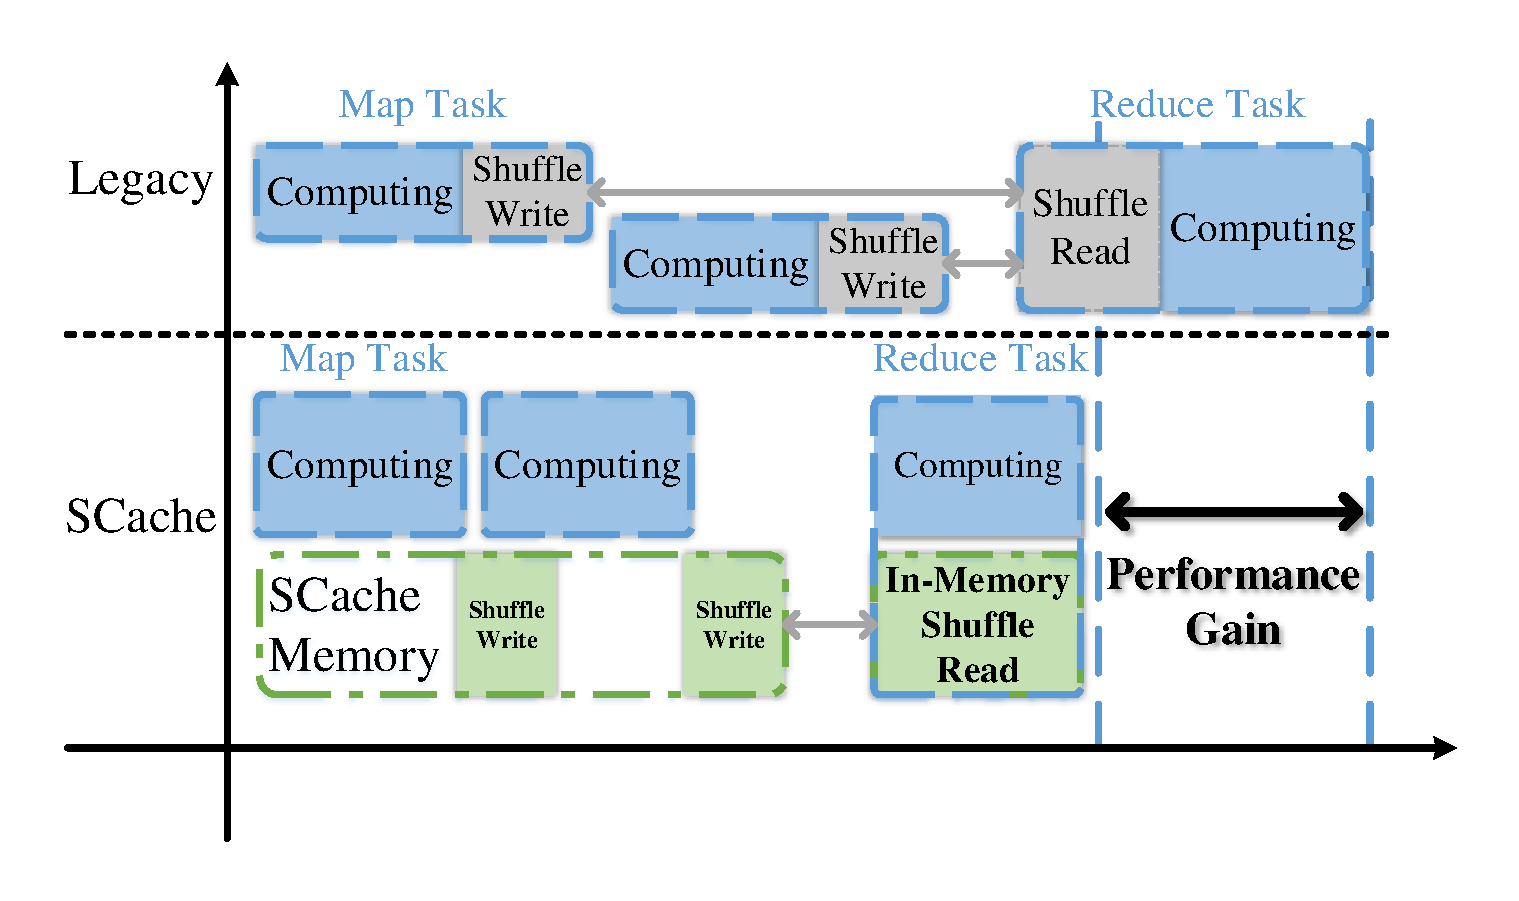
\includegraphics[width=\linewidth]{fig/workflow}
	\caption{Workflow Comparison between Legacy DAG Computing Frameworks and Frameworks with SCache}
	\label{fig:workflow}
\end{figure}

Moreover, the shuffle read phase introduces all-to-all communication pattern across the network, and such network I/O procedure is also poorly coordinated.
Note that the shuffle read phase starts fetching data only after the corresponding reduce task starts.
Meanwhile, the reduce tasks belonging to a same execution phase are scheduled at the same time by default. 
As a result, all the corresponding reduce tasks start fetching shuffle data almost simultaneously.
Such synchronized network communication causes a burst demand for network I/O, which in turn greatly enlarges the shuffle read completion time. 
To desynchronize the network communication, an intuitive way is to launch some tasks in the descendent stage earlier, such as "slow-start" from Hadoop MapReduce\footnote{http://hadoop.apache.com/}. 
However, such early-start is by no means a panacea. 
This is because the early-start always introduces an extra early allocation of the slot leading to a slow execution of the current stage.


%In one word, existing solutions suffer from either inefficient use of network I/O, or a waste of computational resources (i.e., CPU and memory) caused by task pre-launching.

%For example, Apache Hadoop \cite{hadoop} provides an \emph{early start} mechanism that launches reduce tasks after a certain portion (5\% by default) of map tasks has completed, which is adopted in many of the recent works \cite{ihadoop, ishuffle, dynmr}.
% DAG computing framworks deriving from MapReduce \cite{mapreduce} contains a hard barrier between computing stages. The terminology of this barrier is \textit{shuffle}. Shuffle contains two parts on the connecting stages -- \textit{shuffle write} and \textit{shuffle read}. On the side of ancestor stages, \textit{shuffle write} is resoponsible for writing intermediate results to disk. On the side of descendant stage, \textit{shuffle read} fetches intermediate results from remote disks through network. Although highly optimized in other factors, the shuffle of framework is still primitive.  The coarse design of shuffle introduce a significiant performance overhead.
% % design inconsistent
% For instance, a MapReduce trace analysis from Facebook shows that shuffle accounts for 33\% JCT on average, up to 70\% in shuffle-heavy jobs \cite{managing}.
% shuffle operations
% three resource coordinate 不好
% 计算和I/O couple, why
% why disk, reason!!!, 不重视
% common problems

To make things worse, we note that the above deficiencies generally exist in most of the DAG computing frameworks. 
As a result, even we can effectively resolve the above deficiencies by modifying one framework, updating one application at a time is impractical given the sheer number of computing frameworks available today.

% The main defect of current shuffle design is coarse granularity of resource allocation during the task scheduling.
% Nearly all task scheduling algorithms in DAG frameworks use time slotted model. Specifically, when a task is launched, the framework offers it a bundle of resources (i.e. CPU and memory), which are dedicated to this task during the time in its "slot".
% But for a task, the resources demand changes during different phases. The computing phase is CPU and memory intensive. The shuffle, instead, is I/O intensive.
% As shown in the upper part of Figure \ref{fig:workflow}, this "slot" can be released until the map tasks finish \textit{shuffle write} on disk. And the "slot" is occupied when the reduce tasks begin to read shuffle data from remote nodes through network, which is presented as \textit{shuffle read}. This inconsistency between demands and allocation results in a severe resource underutilization, which slow down the framework.

% Another drawback of current shuffle is the synchronized shuffle read. When all the reduce tasks are scheduled, the shuffle fetch of each task starts almost simultaneously, which may cause congestion of network and delay the shuffle read. The straight forward way to avoid network burst is to start reduce tasks earlier. Apache Hadoop \cite{hadoop} provides a mechanism that schedules reduce tasks when a certain portion of map tasks completed. So that the shuffle delay can be mitigated. Other publications also purpose solutions to pre-schedule reduce tasks \cite{ihadoop, ishuffle, dynmr}. However this early scheduling of reduce tasks occupies new task slots, which degrades system performance. To this end, we proposed a question for this cross-frameworks issue, \textit{can we efficiently optimize shuffle without manually change every DAG framework?}




% 针对性的提出这三个点
% three resource coordinate 不好
% 计算和I/O couple, why
% why disk, reason, 不重视
% common problems
% 总起:普适性工具
% pre-fetch but not pre-execute
% byproduct: more balance
% memory instead of disk

% challenge point by point, inside the problem


{\color{blue}
In order to visually analyze above-mentioned resources scheduling, we propose a performance model called \textit{Framework Resources Quantification}(FRQ) model. FRQ model quantifies computing and I/O resources and displays resources scheduling strategy of DAG framework in time dimension. We use FRQ model to assist in analyze the deficiencies of resources scheduling and optimize it. 
FRQ model has five parameters: \textit{Input Data Size, Data Conversion Rate, Computation Round Number, Computation Speed,} and \textit{Shuffle  Speed}.
According to the above five parameters and the scheduling strategy of the DAG framework, FRQ model is able to calculate the execution time of each phase of a computing job. 
Take Apache Hadoop MapReduce as a simple DAG computing example, we use FRQ to model each phases of the computing, including Map, Shuffle, and Reduce.
By revealing the relationships between the various phases, FRQ model assist us in discovering the irrationality of resource scheduling during computing.
I/O resource in Map phase is not fully utilized. Furthermore, due to coupling with reduce phase, shuffle phase delay the execution time of reduce phase. 
This situation will be amplified in shuffle-sensitive tasks.
}

Can we efficiently optimize the data shuffling without significantly changing DAG frameworks?
In this paper, we answer this question in the affirmative with S(huffle)Cache, an open source\footnote{https://github.com/frankfzw/SCache} plug-in system which provides a shuffle-specific optimization for different DAG computing frameworks.
Specifically, SCache takes over the whole shuffle phase from the underlying framework by providing a cross-framework API for both shuffle write and read.
SCache's effectiveness lies in the following two key ideas.
First, SCache decouples the shuffle write and read from both map and reduce tasks.
Such decoupling effectively enables fine-grained resource management and better multiplexing between the computational and I/O resources.
In addition, SCache pre-schedules the reduce tasks \emph{without launching} them and pre-fetches the shuffle data. 
% for the reduce tasks.
Such pre-scheduling and pre-fetching effectively overlap the network transfer time, desynchronize the network communication, 
and avoid the extra early allocation of slots.
%In this paper, we introduce S(huffle)Cache, an plugin system to remove shuffle latency for DAG frameworks. SCache takes over the management of shuffle and I/O resources to acheive a fine granularity scheduling of tasks. In addition, SCache pre-schedules the reduce tasks without launching them and perform shuffle data pre-fetch to break the synchronization of shuffle fetch. In order to provide a general optimization for different DAG frameworks, SCache decouple the shuffle process from computing and  provide a cross-frameworks API for shuffle write and read.

The workflow of a DAG framework with SCache is presented in Figure \ref{fig:workflow}. 
SCache replaces the disk operations of shuffle write by the memory copy in map tasks. 
The slot is released after the memory copy. 
The shuffle data is stored in the reserved memory of SCache until all reduce tasks are pre-scheduled. 
Then the shuffle data is pre-fetched according to the pre-scheduling results.  
The application-context-aware memory management caches the shuffle data in memory before launching the reduce task.
By applying these optimizations, SCache can help the DAG framework achieve a significant performance gain.  

The main challenge to achieve this optimization is \textit{pre-scheduling reduce tasks without launching}. 
% It is not critical for the simple DAG computing such as Hadoop MapReduce \cite{mapreduce}. 
First, the complexity of DAG can amplify the defects of na\"{i}ve scheduling schemes. 
In particular, randomly assigning reduce tasks might result in a collision of two heavy tasks on one node. 
This collision can aggravate data skew, thus hurting the performance. 
Second, pre-scheduling without launching violates the design of most frameworks that launch a task after scheduling.
To address the challenges, we propose a heuristic task pre-scheduling scheme with shuffle data prediction and a task co-scheduler (Section \ref{opt}).

Another challenge is the \textit{in-memory data management}. 
To prevent shuffle data touching the disk, SCache leverages extra memory to store the shuffle data. 
% However, the memory is a precious resource for DAG computing. 
To minimize the reserved memory while maximizing the performance gain, we propose two constraints: all-or-nothing and context-aware (Section \ref{memorymanage}).
%The memory management scheme follows these two contraints to switch shuffle data blocks on and off reserved memory.

% {\color{red}
% We have implemented SCache and a customized Apache Spark \cite{apachespark}. The performance of SCache is evaluated with both simulations and testbed experiments on a 50-node Amazon EC2 cluster. We conduct basic test GroupByTest. We also evaluate Terasort \cite{spark-tera} benchmark and standard workloads like TPC-DS \cite{tpcds} for multi-tenant modeling. In a nutshell, SCache can eliminate explicit shuffle process by at most $89\%$ in varied application scenarios. More impressively, SCache reduces $~40\%$ of overall completion time of TPC-DS queries on average.
% }

{\color{blue}
We have implemented SCache, a customized Apache Spark \cite{apachespark} and a customized Apache Hadoop. We have also designed a performance model called \textit{Framework Resources Quantification}(FRQ) model to analyze the shuffle optimization of SCache and calculate the execution time of each phase of computing job. The performance of SCache is evaluated with both simulations and testbed experiments on a 50-node Amazon EC2 cluster on both Apache Spark and Apache Hadoop. On Apache Spark, we conduct basic test GroupByTest. We also evaluate Terasort\footnote{https://github.com/ehiggs/spark-terasort} benchmark and standard workloads like TPC-DS\footnote{http://www.tpc.org/tpcds/} for multi-tenant modeling. On Apache Hadoop, we focus on Terasort benchmark. In a nutshell, SCache can eliminate explicit shuffle process by at most $89\%$ in varied application scenarios. More impressively, SCache reduces $~40\%$ of overall completion time of TPC-DS queries on average on Apache Spark. On Apache Hadoop, Scache optimize end-to-end Terasort completion time by 15\%.
}
\section{Background and Observations}

In this section, we first study the typical shuffle characteristics (\ref{shuffle pattern}), and then spot the opportunities to achieve shuffle optimization (\ref{observation}).
\subsection{Characteristic of Shuffle} \label{shuffle pattern}

In large scale data parallel computing, shuffle is designed to achieve an all-to-all data transfer among nodes. 
For a clear illustration, we use \textit{map tasks} to define the tasks that produce shuffle data and use \textit{reduce tasks} to define the tasks that consume shuffle data.
% Note that one task may have both shuffle data generation and consumption in modern DAG framework. These tasks contain characteristic of both map task and reduce task. But these tasks won't change the behavior of shuffle. To avoid ambiguity, in the following paper, we will only use term of map task to represent those who produce shuffle output, and reduce task to represent those who consume shuffle output.
% \begin{figure}
% 	\centering
% 	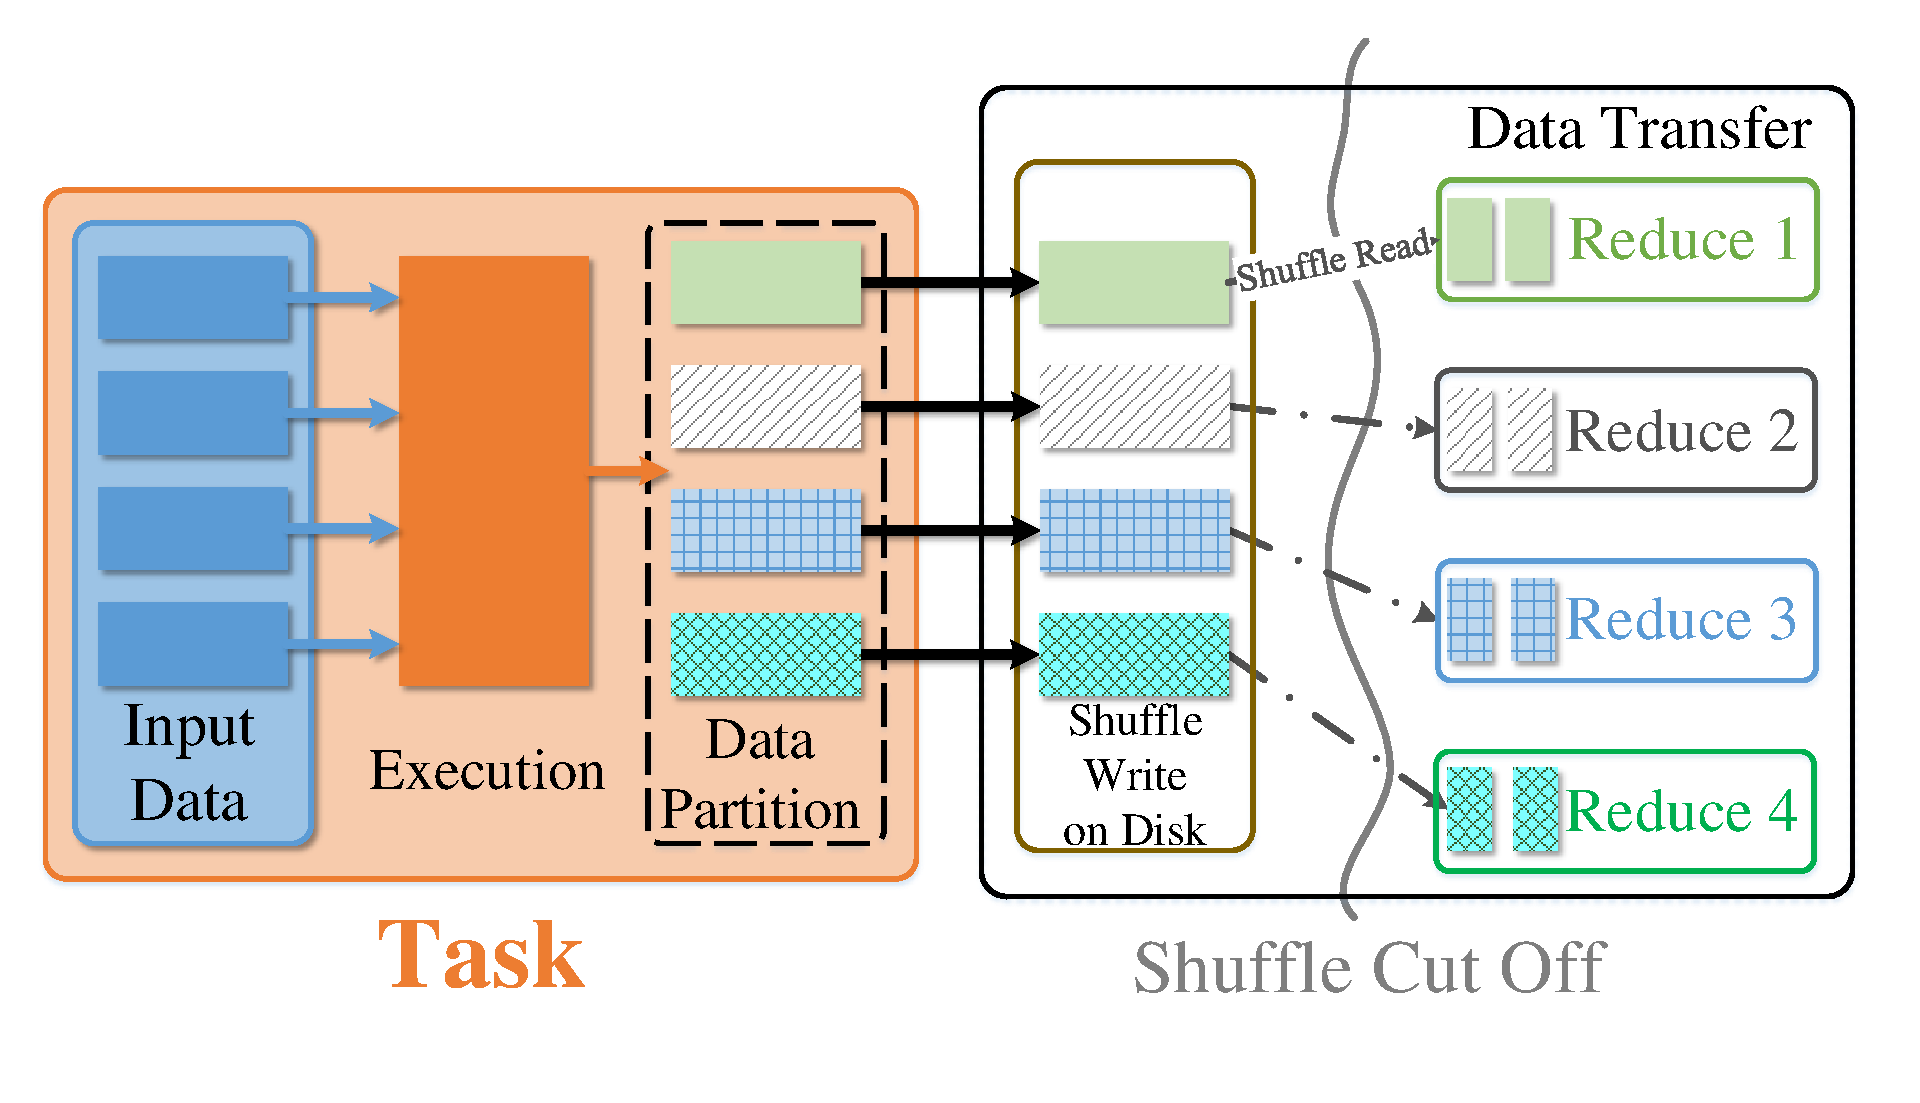
\includegraphics[width=\linewidth]{fig/shuffle_process}
% 	\caption{Shuffle Overview}
% 	\label{fig:shuffle_process}
% \end{figure}

\textbf{Overview of shuffle process}. 
Each map task partitions the result data (key, value pair) into several buckets according to the partition function (e.g., hash). 
The total number of buckets equals the number of reduce tasks in the successive step.
% shuffle data is produced by \textit{data partition}. For \textit{data partition}, 
The shuffle process can be further split into two parts: \textit{shuffle write} and \textit{shuffle read}. 
Shuffle write starts at the end of a map task and writes the partitioned map output data to local persistent storage. 
Shuffle read starts at the beginning of a reduce task and fetches the partitioned data from remote as its input. 

%In short, shuffle is loosely coupled with application context and it's I/O intensive.
\textbf{Impact of shuffle process}. Shuffle is I/O intensive, which might introduce a significant latency to the application. 
Reports show that 60\% of MapReduce jobs at Yahoo! and 20\% at Facebook are shuffle-heavy workloads \cite{shufflewatcher}. 
For those shuffle-heavy jobs, the shuffle latency may even dominate Job Completion Time (JCT).
For instance, a MapReduce trace analysis from Facebook shows that shuffle accounts for 33\% JCT on average, up to 70\% in shuffle-heavy jobs \cite{managing}.
% Besides, the completion time of shuffle correlates with the performance of storage devices, network and even applications.
% This variation may bring a huge challenge for operators to find the correct configuration of the DAG framework.

\subsection{Observations} \label{observation}
% Of course, shuffle is unavoidable in a DAG computing process. 
Can we mitigate or even remove the overhead of shuffle? 
To find the answers, we ran some typical Spark applications on a 5-node \texttt{m4.xlarge} EC2 cluster and analyzed the design and implementation of shuffle in some DAG frameworks.
Here we present the hardware utilization trace of one node running Spark's \textit{GroupByTest} in Figure \ref{fig:util} as an example. 
This job has 2 rounds of tasks for each node.
The \textit{Map Execution} is marked from the launch time of the first map task to the execution end time of the last one. 
The \textit{Shuffle Write} is marked from the beginning of the first shuffle write in the map stage. 
The \textit{Shuffle Read and Reduce Execution} is marked from the launch time of the first reduce task.
% Figure \ref{fig:util} reveals the performance information of two stages that are connected by shuffle. By analyzing the trace with Spark source code \cite{sparksource}, we propose the following observations.
% \begin{figure*}
% 	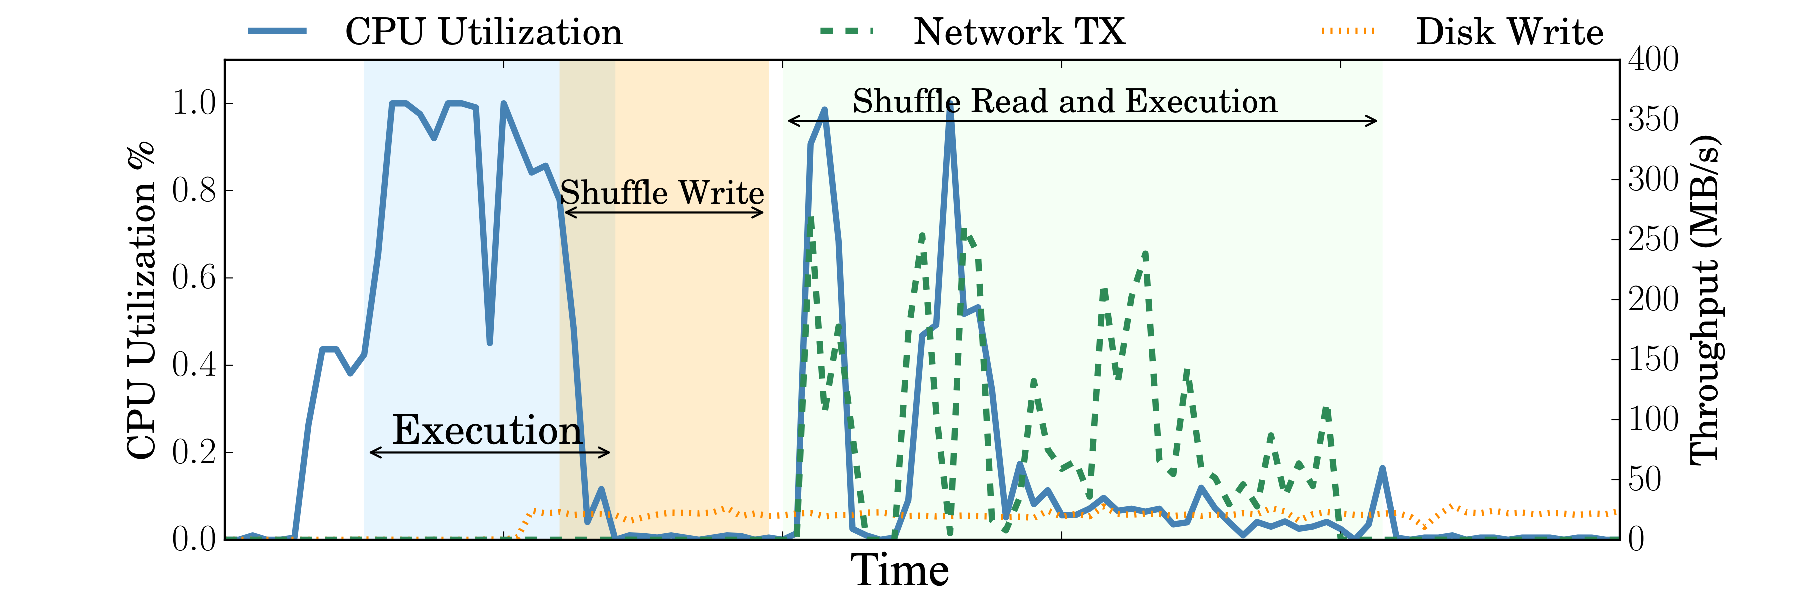
\includegraphics[width=\textwidth]{fig/util}
% 	\caption{CPU utiliazation and I/O throughput of a node during a Spark single shuffle application}
% 	\label{fig:util}
% \end{figure*}
\subsubsection{Coarse Granularity Resource Allocation}
When a slot is assigned to a task, it will not be released until the task completes (i.e., the end of shuffle write in Figure \ref{fig:util}). 
On the reduce side, the network transfer of shuffle data introduces an explicit I/O delay during shuffle read (i.e., the beginning of shuffle read and execution in Figure \ref{fig:util}). 
Meanwhile, both shuffle write and shuffle read occupy the slot without significantly involving CPU as presented in Figure \ref{fig:util}. 
The current coarse slot-task mapping results in an imbalance between task's resource demand and slot allocation thus decreasing the resource utilization. 
Unfortunately this defect exists not only in Spark \cite{apachespark} but also Hadoop MapReduce and Apache Tez \cite{tez}. 
A finer granularity resource allocation scheme should be provided to reduce these delays. 

\subsubsection{Synchronized Shuffle Read}
Almost all reduce tasks start shuffle read simultaneously. 
The synchronized shuffle read requests cause a burst of network traffic. 
As shown in Figure \ref{fig:util}, 
the data transfer causes a high demand of network bandwidth, which may result in network congestion and further slow down the network transfer.
It also happens in other frameworks that follow Bulk Synchronous Parallel (BSP) paradigm, such as Hadoop MapReduce, Dryad \cite{dryad}, etc.
% The previous work \cite{coflow, managing} also proves that the network transfer can introduce significant overhead in DAG computing.

\begin{figure}
	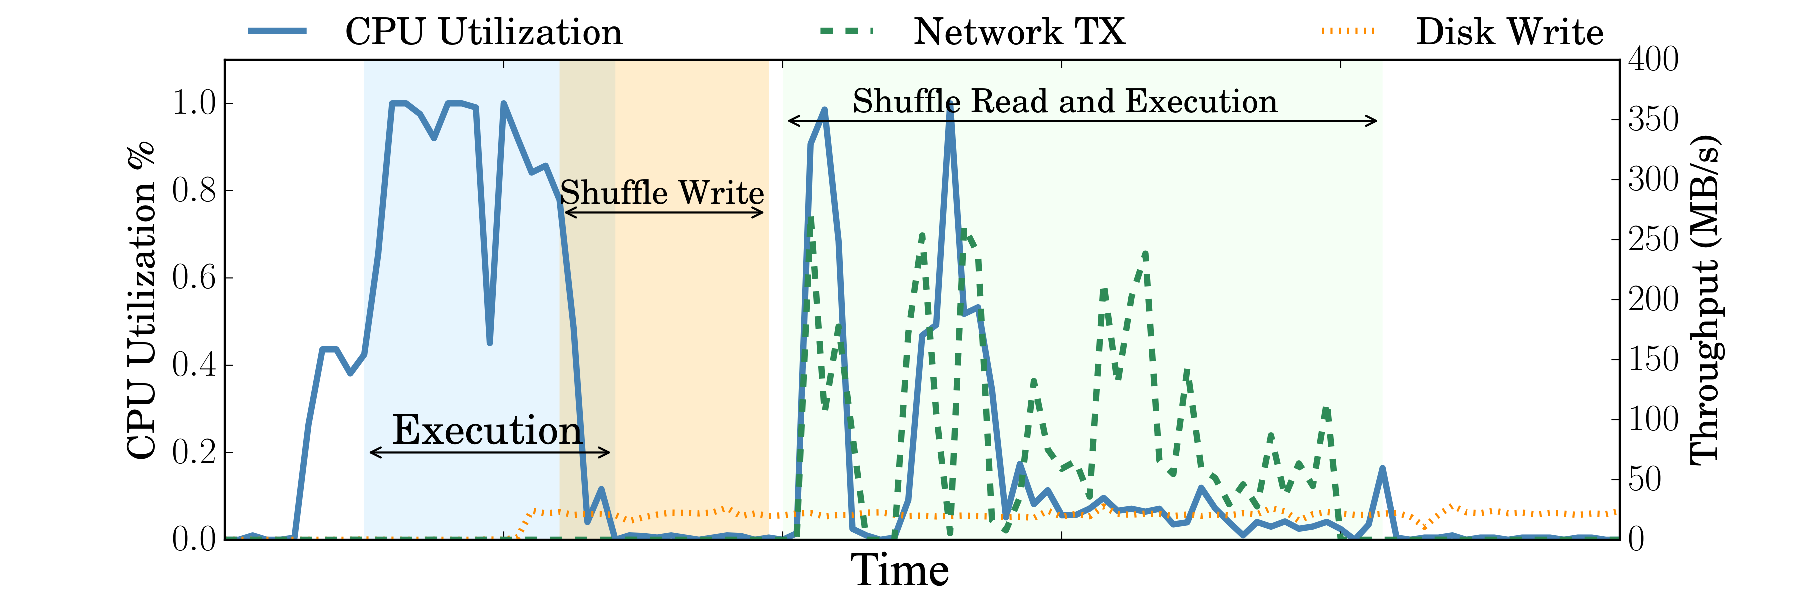
\includegraphics[width=\linewidth]{fig/util}
	\caption{CPU utilization and I/O throughput of a node during a Spark single shuffle application}
	\label{fig:util}
	\vspace{-1em}
\end{figure}

\subsubsection{Inefficient Persistent Storage Operation}
At first, both shuffle write and read are tightly coupled with task execution, which results in a blocking I/O operation. 
This blocking I/O operation along with synchronized shuffle read may introduce significant latency, especially in an I/O performance bounded cluster.
Besides, the legacy of storing shuffle data on disk is inefficient in modern clusters with large memory. 
Compared to input dataset, the size of shuffle data is relatively small. 
For example, the shuffle size of Spark Terasort\footnote{https://github.com/ehiggs/spark-terasort} is less than 25\% of input data. 
The data reported in \cite{makingsense} also show that the amount of data shuffled is less than the input data by as much as 10\%-20\%. 
On the other hand, memory based distributed storage systems have been proposed \cite{memcached, tachyon, ramcloud} to move data back to memory, 
but most of the DAG frameworks still store shuffle data on disks (e.g., Spark \cite{apachespark}, Hadoop MapReduce, Dryad \cite{dryad}, etc).
We argue that the memory capacity is large enough to store the short-living shuffle data with cautious management.

\subsubsection{Multi-round Tasks Execution}\label{multi}
Both experience and DAG framework manuals recommend that multi-round execution of each stage will benefit the performance of applications.
For a cluster with $n$ slots, the number of tasks should be $n \times k (k \geq 1)$. 
For example, Hadoop MapReduce Tutorial\footnote{http://hadoop.apache.org/docs/current/hadoop-mapreduce-client/hadoop-mapreduce-client-core/MapReduceTutorial.html} suggests that \textit{10-100 maps} per-node and \textit{0.95 or 1.75 $\times$ number of nodes $\times$ number of maximum container reduces} per-node seem to be the right level of parallelism. 
Spark configuration also recommends $2\text{-}3$ tasks per CPU core\footnote{http://spark.apache.org/docs/1.6.2/configuration.html} (i.e., $k = 2\text{-}3$).

Since the shuffle data becomes available as soon as the end of a task's execution, 
and the network is idle during the map stage ("Network TX" during map stage in Figure \ref{fig:util}), 
the property of multi-round tasks can be leveraged to hide the cost by starting shuffle data transfer at the end rounds of map tasks. 
% optimize the shuffle read operations if the destination host of the shuffle data can be predicted a priori. 
% There are at least two persistent storage operations for each shuffle data block. At first, Spark will write shuffle data to the persistent storage after map task execution (i.e. \textit{shuffle write} in Figure \ref{fig:util}). During the \textit{shuffle read}, Spark will read shuffle data from remote and local persistent storage, which is the second operation. The persistence of shuffle data was designed for fault tolerance. But we believe it is not necessary for today's cluster. Recall that shuffle data only exist in a short time scale. But the Mean Time To Failure (MTTF) for a server is counted in the scale of year \cite{tachyon}, which is exponential compared with the duration of a shuffle. In addition, the capacity of memory and network has been increasing rapidly in recent years. As a result, numbers of memory based distributed storage system have been proposed \cite{memcached, tachyon, ramcloud}. On the other hand, the size of shuffle data is relatively small. For example, shuffle size of Spark Terasort \cite{spark-tera} is less than 25\% of input data. The data reported in  \cite{makingsense} also shows that the amount of data shuffled is less than input data, by as much as 10\%-20\%. We argue that removing persistent storage and using memory to achieve shuffle fault tolerance is feasible and efficient.

Based on these observations, most of the DAG frameworks share the execution paradigm as well as the expense of shuffle process. 
To mitigate the shuffle overhead, we propose an optimization that starts shuffle read ahead of reduce stage to overlap the I/O operations in multi-round map tasks, and uses memory to store the shuffle data. 
To achieve this optimization:
\begin{itemize}
	\item Shuffle process should be decoupled from task execution to achieve a fine granularity scheduling scheme.
	\item Reduce tasks should be pre-scheduled without launching to achieve shuffle data pre-fetching.
	\item Shuffle process should be taken over and managed outside DAG frameworks to achieve a cross-framework optimization.
\end{itemize}
% In the following section, we elaborate the methodologies to achieve three design goals.

\section{Shuffle Optimization}
\label{opt}
This section presents the detailed methodologies to achieve the three design goals. 
The out-of-framework shuffle data management is used to decouple shuffle from execution and provide a cross-framework optimization. 
Two heuristic algorithms (Algorithm \ref{hminheap}, \ref{mhminheap}) and a co-scheduler is used to achieve shuffle data pre-fetching without launching tasks.
\begin{figure}
	\centering
	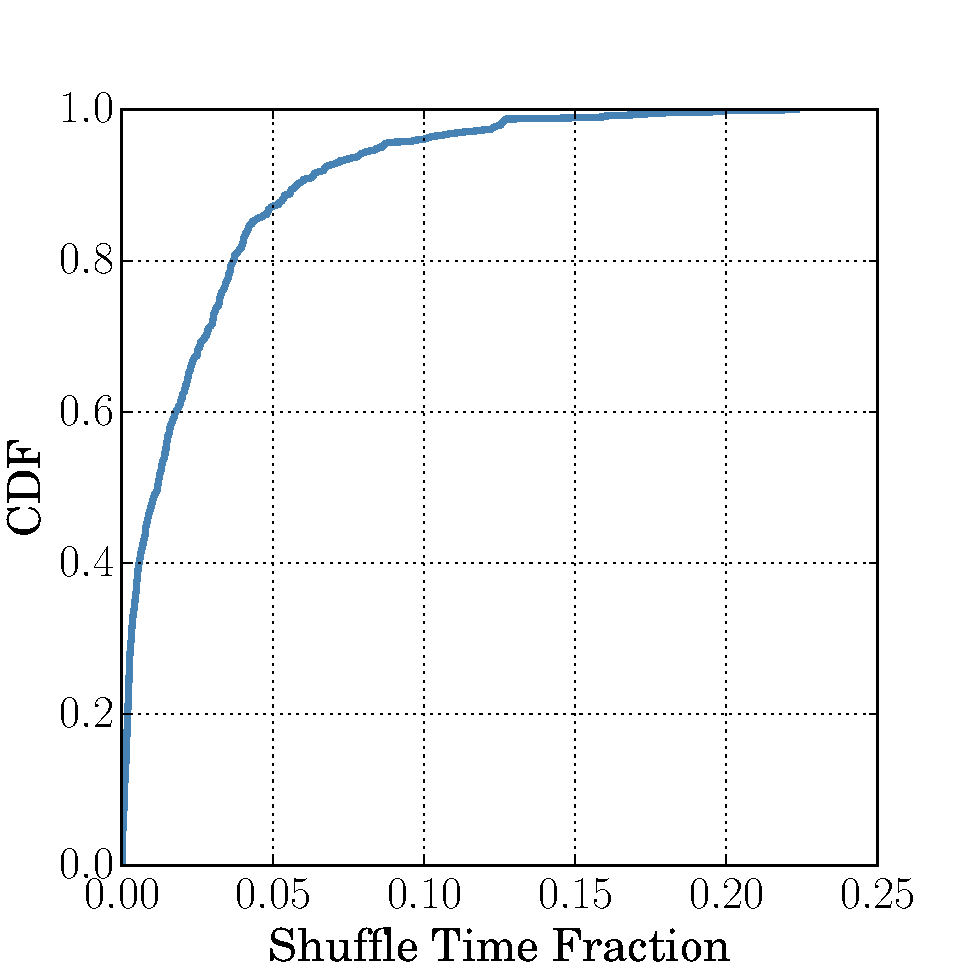
\includegraphics[width=0.5\linewidth]{fig/reduce_cdf}
	\caption{Shuffle Time Fraction CDF of OpenCloud Trace}
	\label{fig:cdf}
	\vspace{-1em}
\end{figure}
\subsection{Decouple Shuffle from Execution}
% \ifrevision
% \reversemarginpar
% \marginpar{B1,C2}
% \fi
To achieve the decoupling of map tasks and reduce tasks, the original shuffle write and read implementation in the current frameworks should be modified to apply the API of SCache.
% During shuffle write of map tasks, the partitioned shuffle data blocks will be written on the disks.
% Each block contains a part of input data of a particular reduce task. 
To prevent the release of a slot being blocked by shuffle write,  
SCache provides a disk-write-like API named $putBlock$ to handle the storage of partitioned shuffle data blocks produced by a map task.
Inside the $putBlock$, SCache uses memory copy to move the shuffle data blocks out of map tasks and store them in the reserved memory.
After the memory copy, the slot will be released immediately.

From the perspective of reduce task, SCache provides an API named $getBlock$ to replace the original implementation of shuffle read. 
With the precondition of shuffle data pre-fetching, 
the $getBlock$ leverages the memory copy to fetch the shuffle data from the local memory of SCache.
% Instead, the original implementation of shuffle read will trigger an all-to-all network transfer that keeps CPU idle.
%To this end, all I/O operations are managed outside of the DAG framework, and the slot is occupied only by the CPU intensive phases of task.
\subsection{Pre-schedule with Application Context}
The pre-scheduling and pre-fetching are the most critical aspects of the optimization. 
The task-node mapping is not determined until tasks are scheduled by the scheduler of DAG framework. 
Once the tasks are scheduled, the slots will be occupied to launch them. 
On the other hand, the shuffle data cannot be pre-fetched without the awareness of task-node mapping.
We propose a co-scheduling scheme with two heuristic algorithms (Algorithm \ref{hminheap}, \ref{mhminheap}). 
That is, the task-node mapping is established a priori, and then it is enforced by the co-scheduler when the DAG framework starts task scheduling. 
% We explore several pre-scheduling schemes in different scenarios, and evaluate the performance calculating the improvement of reduce tasks completion time with trace of OpenCloud \cite{opencloudtrace}. We first emulate the scheduling algorithm of Spark to schedule the reduce tasks of one job, and take the bottleneck of the task set as the completion time. Then we remove the shuffle read time as the assumption of shuffle data pre-fetch and emulate under different schemes. The result is shown in \ref{fig:sim}.
% \begin{figure*}
% 	\centering
% 	\begin{minipage}{0.34\linewidth}
% 		\begin{figure}[H]
% 			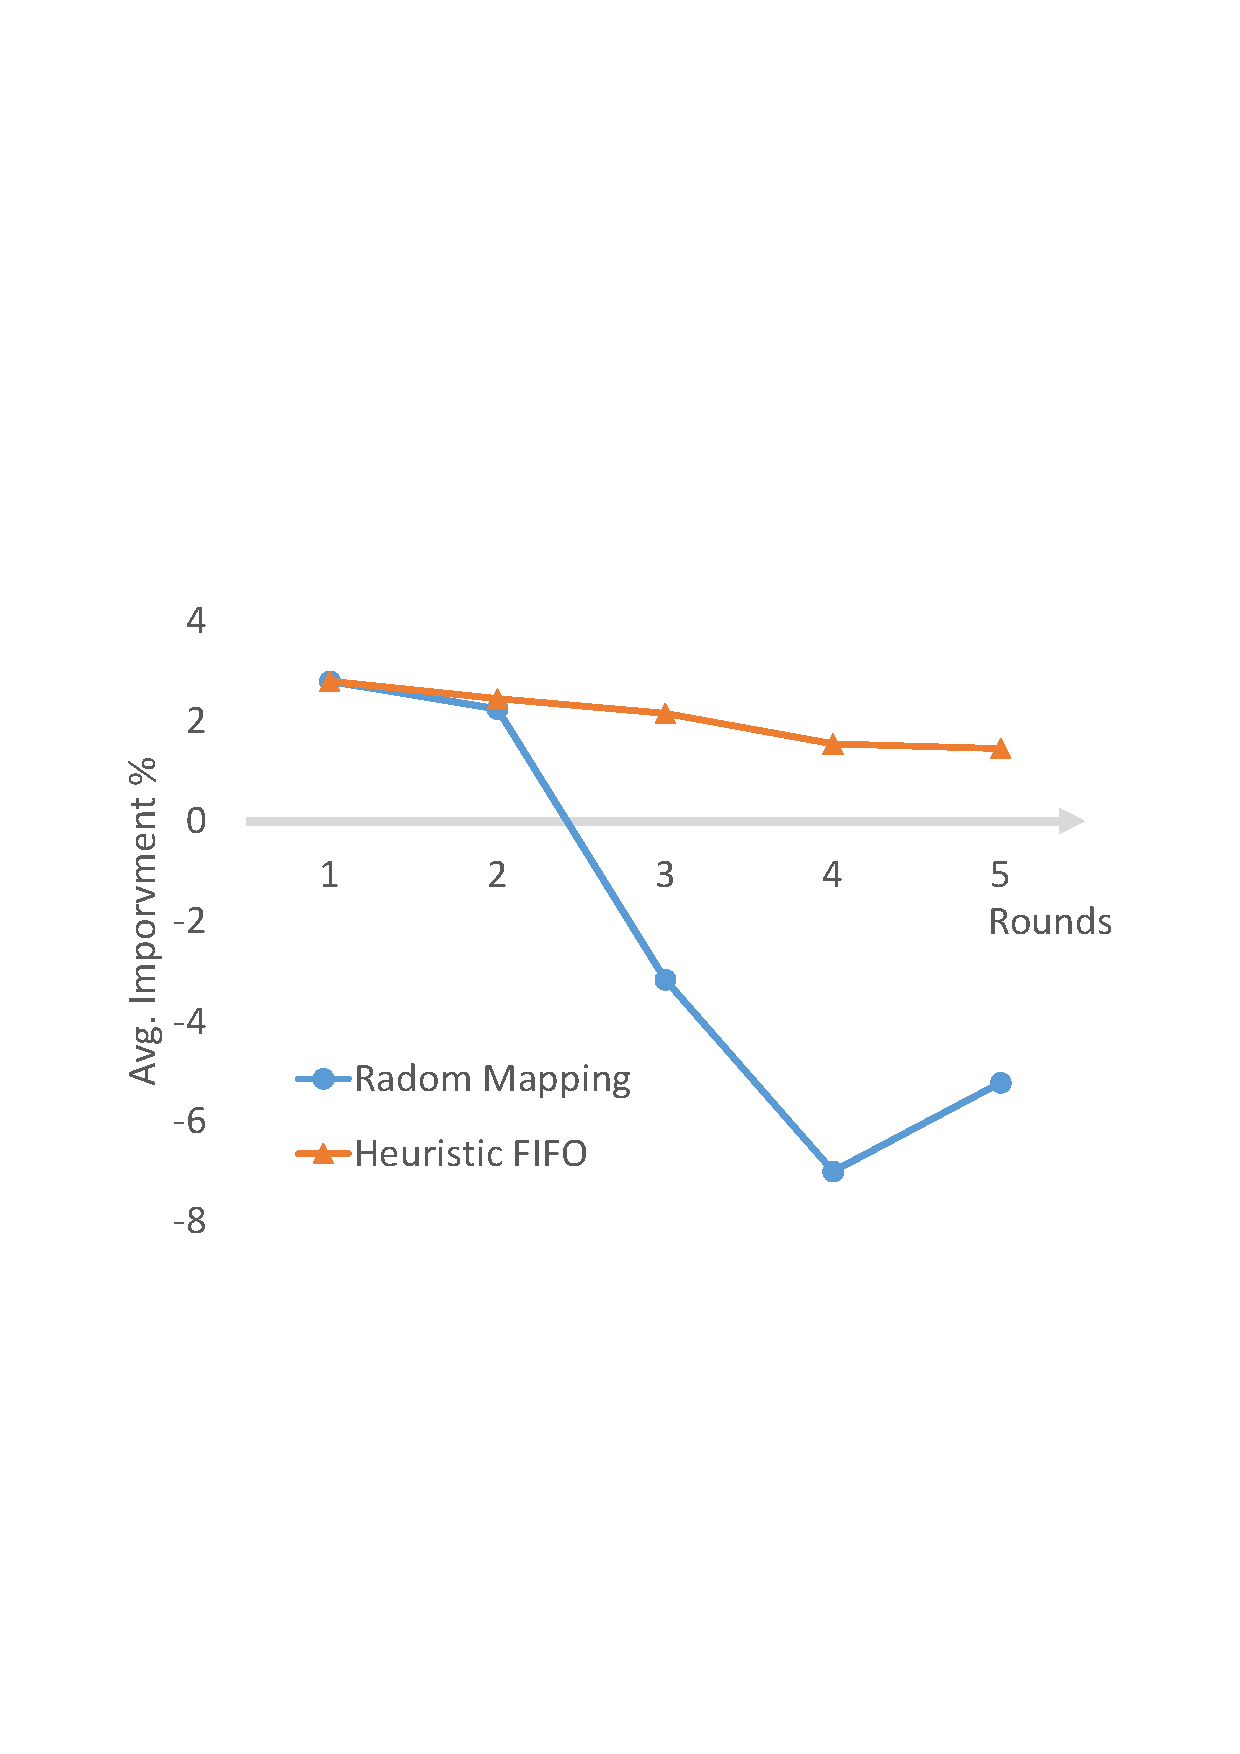
\includegraphics[width=\textwidth]{fig/shuffle_size}
% 			\caption{Shuffle Size Comparing with Input Size}
% 			\label{fig:shuffle_size}
% 		\end{figure}
% 	\end{minipage}
% 	\begin{minipage}{0.65\linewidth}
% 		\begin{figure}[H]
% 			\begin{subfigure}{0.5\textwidth}
% 				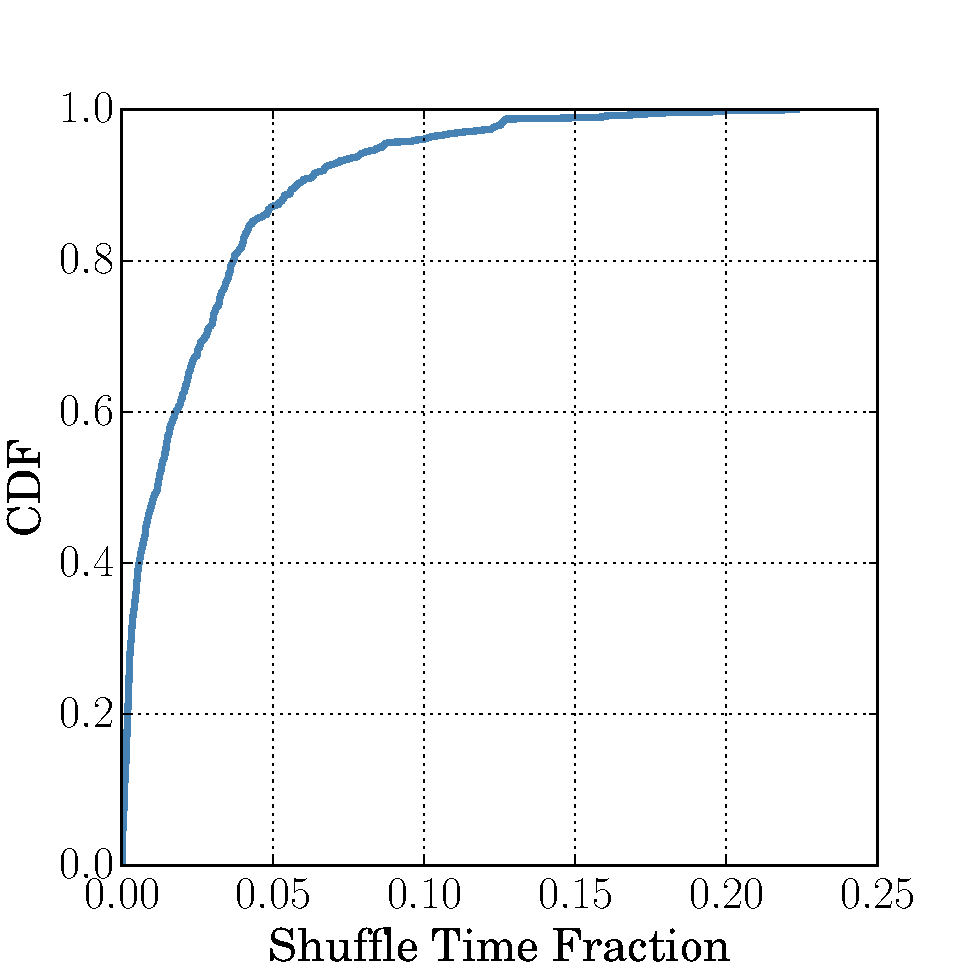
\includegraphics[width=\linewidth]{fig/reduce_cdf}
% 				\caption{Shuffle Time Fraction CDF}
% 				\label{fig:cdf}
% 			\end{subfigure}	
% 			\begin{subfigure}{0.5\textwidth}
% 				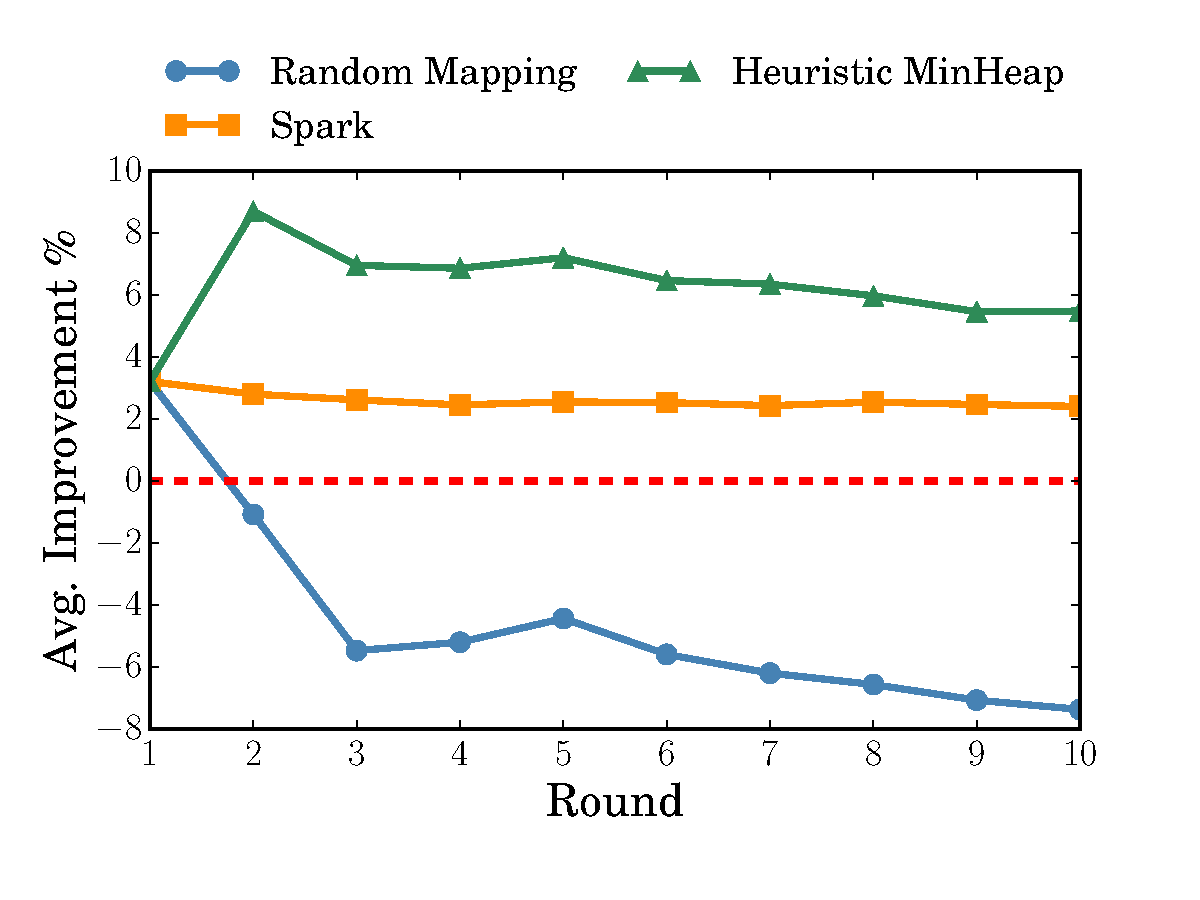
\includegraphics[width=\linewidth]{fig/sim}
% 				\caption{Stage Completion Time Improvement}
% 				\label{fig:sim}
% 			\end{subfigure}	
% 			\caption{Emulate Result of OpenCloud Trace}
% 		\end{figure}
% 	\end{minipage}
% \end{figure*}
% \begin{figure}
\subsubsection{Problem of Random Mapping}\label{randomassign}
The simplest way of pre-scheduling is mapping tasks to nodes randomly and evenly. 
In order to evaluate the effectiveness of random mapping, we use traces from OpenCloud\footnote{\label{fn:trace}http://ftp.pdl.cmu.edu/pub/datasets/hla/dataset.html} for the simulation.
Note that most of the traces from OpenCloud are shuffle-light workload as shown in Figure \ref{fig:cdf}. 
The average shuffle read time is 3.2\% of total reduce completion time.
\begin{figure}
	\centering
	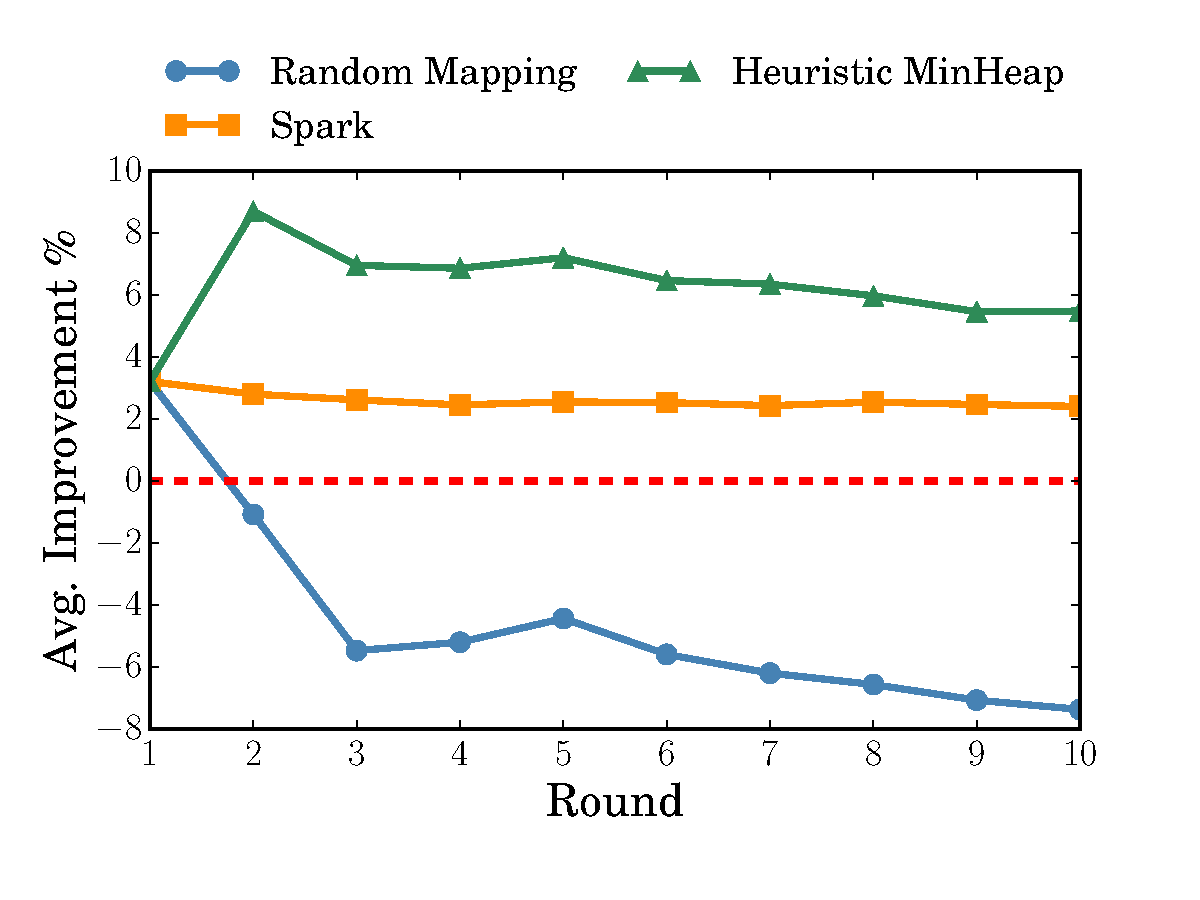
\includegraphics[width=0.66\linewidth]{fig/sim}
	\caption{Stage Completion Time Improvement of OpenCloud Trace}
	\label{fig:sim}
	\vspace{-1em}
\end{figure}
As shown in Figure \ref{fig:sim}, the baseline (i.e., red dotted line) is the stage completion time with Spark FIFO scheduling algorithm. 
We then remove the shuffle read time of each task and run the simulation under three scheduling schemes: random mapping, Spark FIFO, and our heuristic MinHeap.
Random mapping works well when there is only one round of tasks, but the performance drops as the round number grows. 
This is because that data skew commonly exists in data-parallel computing \cite{skewtune, reining, gufler2012load}. 
Several heavy tasks may be assigned to the same node, thus slowing down the whole stage. 
In addition, randomly assigned tasks also ignore the data locality between shuffle map output and reduce input, which may introduce extra network traffic in cluster.
\begin{figure}
	\centering
	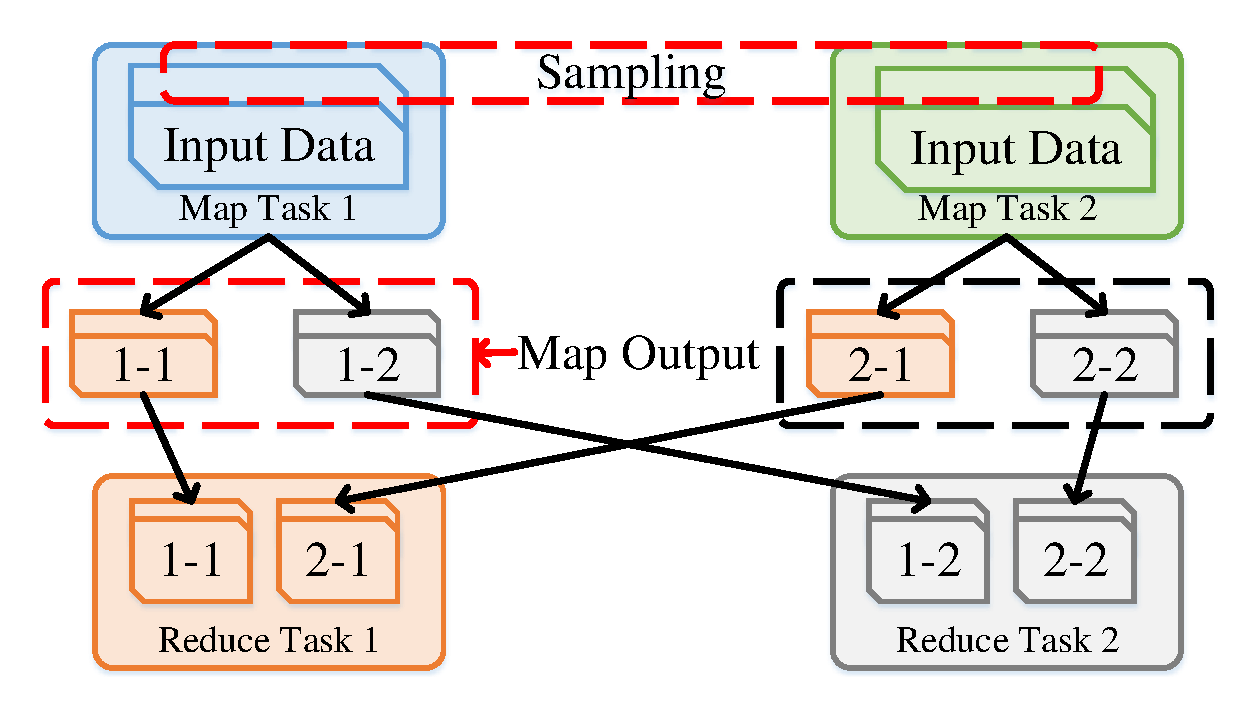
\includegraphics[width=0.75\linewidth]{fig/shuffle}
	\caption{Shuffle Data Prediction}
	\label{fig:shuffle}
	\vspace{-1em}
\end{figure}
\begin{figure*}
	\centering
	\begin{subfigure}[b]{0.31\linewidth}
		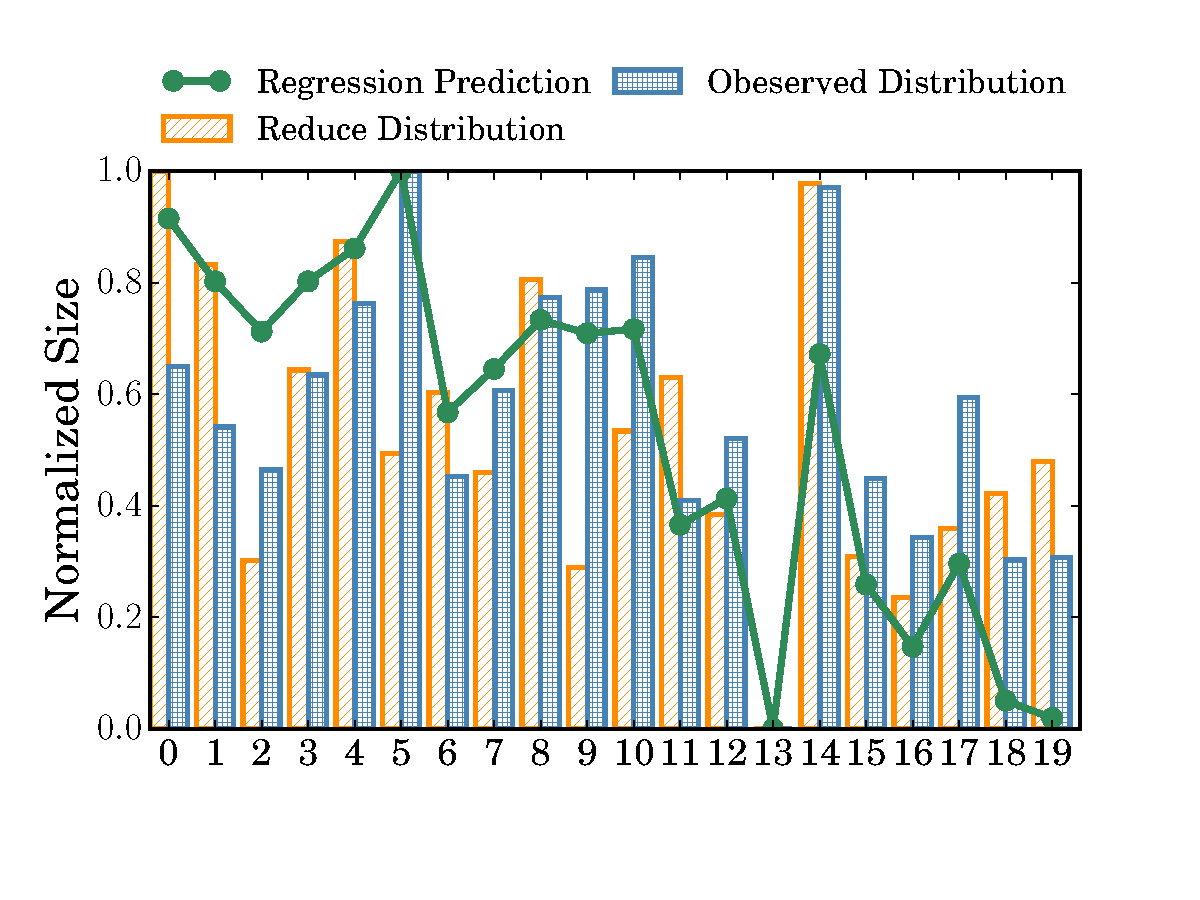
\includegraphics[width=\linewidth]{fig/hash_pre}
		\caption{Linear Regression Prediction of Hash Partitioner}
		\label{fig:hash_pre}
	\end{subfigure}
	\begin{subfigure}[b]{0.31\linewidth}
		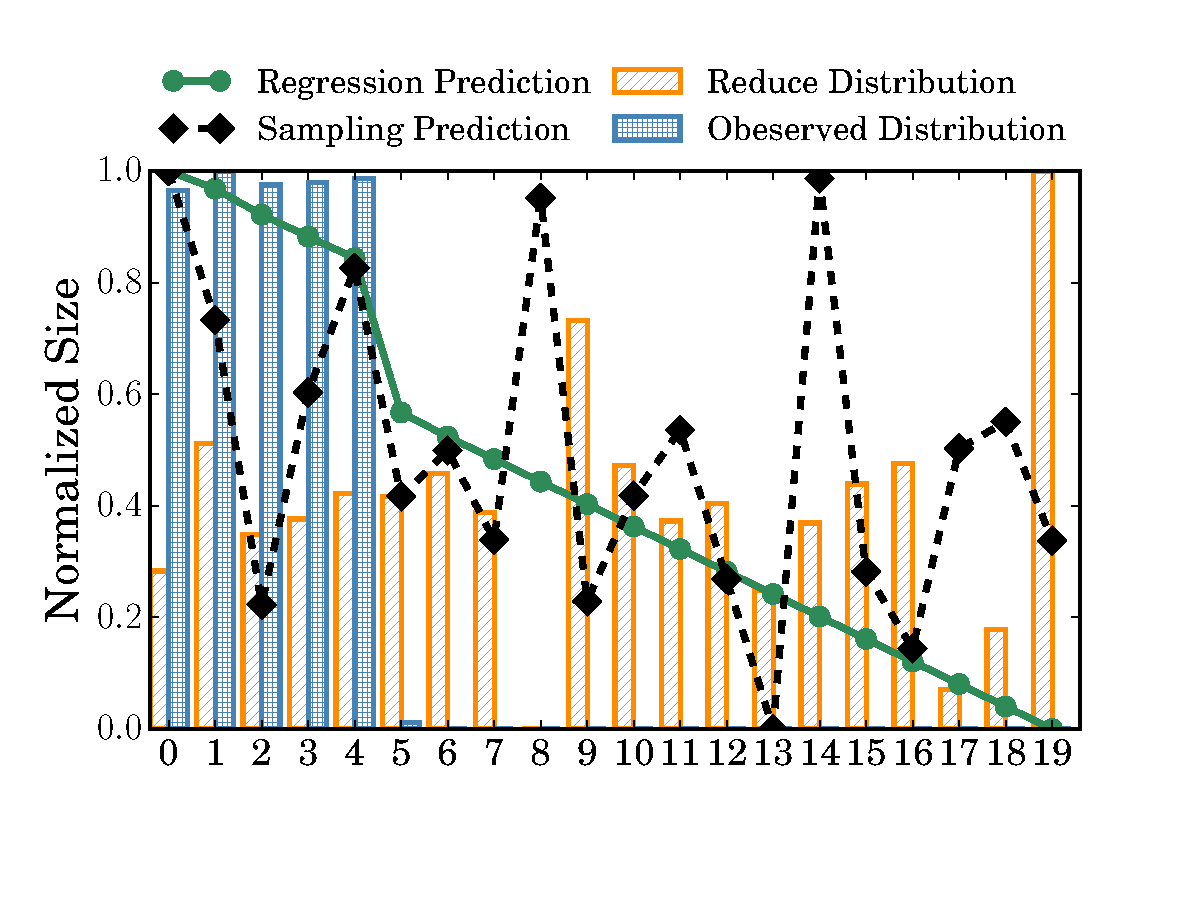
\includegraphics[width=\linewidth]{fig/range_pre_sample}
		\caption{Linear Regression and Sampling Prediction of Range Partitioner}
		\label{fig:range_pre_sample}
	\end{subfigure}
	\begin{subfigure}[b]{0.31\linewidth}
		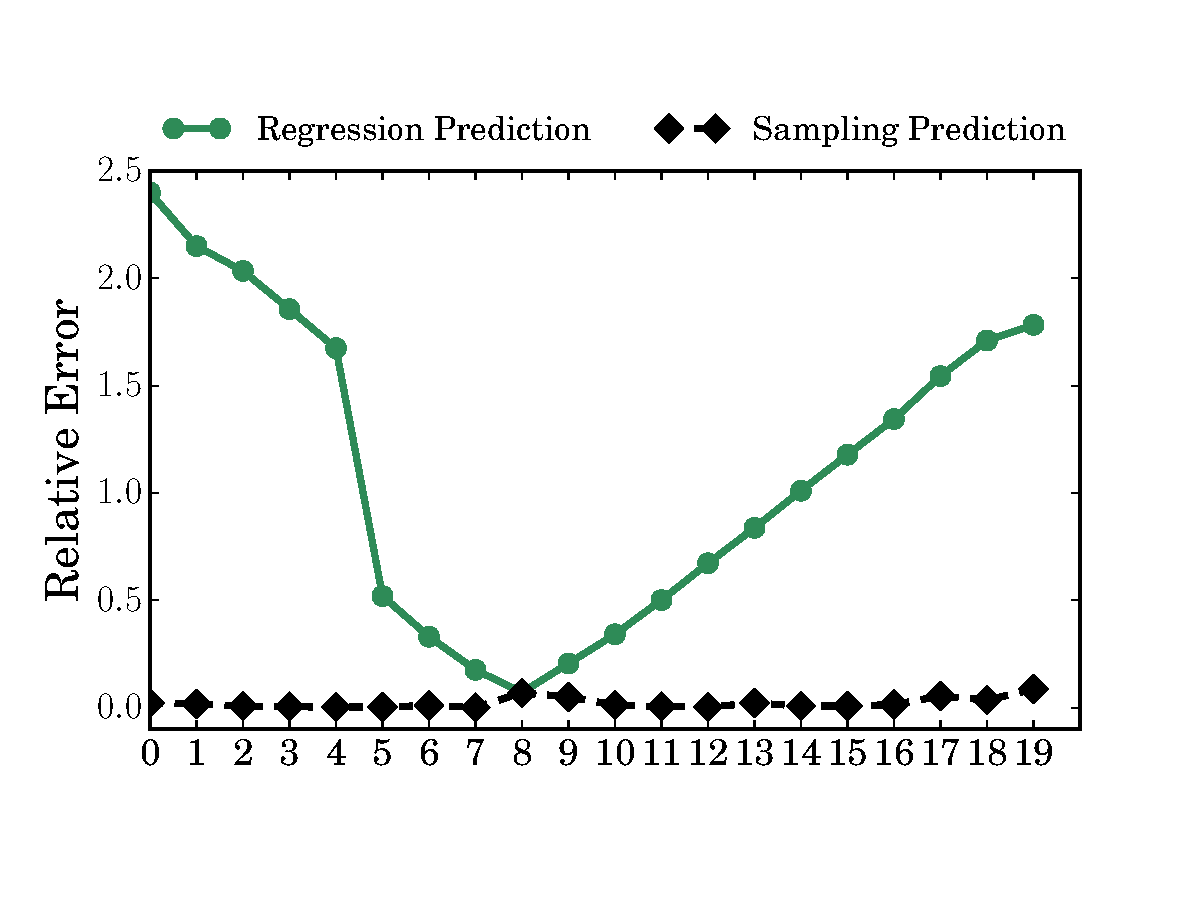
\includegraphics[width=\linewidth]{fig/prediction_relative_error}
		\caption{Prediction Relative Error of Range Partitioner}
		\label{fig:prediction_relative_error}
	\end{subfigure}
	\caption{Reduction Distribution Prediction}
	\label{fig:dis}
	\vspace{-1em}
\end{figure*}

\subsubsection{Shuffle Output Prediction}\label{shuffleprediction}
% \ifrevision
% \marginpar{B2,E7}
% \fi
The problem of random mapping is obviously caused by application context (e.g., shuffle data size) ignorance. 
Note that a balanced schedule decision can be made under the consideration of the size of each reduce task, and the size of a reduce task produced by one shuffle $reduceSize_i = \sum_{j=0}^{m} {BlockSize_{ji}}$, 
where the $m$ is the number of map tasks that can be easily extracted from DAG information; 
$BlockSize_{ji}$ represents the size of block which is produced by map $task_j$ for reduce $task_i$ (e.g., block `1-1' in Figure \ref{fig:shuffle}). 
The final sizes of reduce tasks can be calculated by aggregating $reduceSize_i$ by reduce ID among all shuffle dependencies. 
So the pre-scheduling can be made if the "prediction" of size of shuffle block is practical.
% \hlyellow{
% The shuffle size of each reduce task is decided by input data, map task computation, and hash partitioner. 
% Each map task produces a data block for each reduce task. 
% }
% The size of each reduce partition can be calculated $reduceSize_i = \sum_{j=0}^{m} {BlockSize_{ji}}$ ($m$ is the number of map tasks). 
% $BlockSize_{ji}$ represents the size of block which is produced by map $task_j$ for reduce $task_i$ (e.g., block `1-1' in Figure \ref{fig:shuffle}).
% \ifrevision
% \reversemarginpar
% \marginpar{B2,D6,D8}
% \fi

For the most DAG applications with random large scale input, 
the $BlockSize_{ji}$ in a particular shuffle can be predicted with decent accuracy by liner regression model (i.e., equation \ref{linearregresion}) based on observation that the ratio of map output size and input size are invariant given the same job configuration \cite{guo2017ishuffle, predict}: 
\begin{equation}
\label{linearregresion}
\begin{aligned}
	BlockSize_{ji} = a \times inputSize_j + b
\end{aligned}
\end{equation}
The $inputSize_j$ is the input size of $j$th map task. 
The $a$ and $b$ can be determined using the observed $inputSize_j$ and $BlockSize_{ji}$.

Though the linear regression is stable in most scenarios, it can fail in some uncertainties introduced by sophisticated frameworks like Spark \cite{apachespark}.  
For instance, the customized partitioner may result in large inconsistency between observed map output blocks distribution and the final reduce input distribution. 
We present two particular examples with 20 tasks respectively in Figure \ref{fig:hash_pre} and Figure \ref{fig:range_pre_sample}. 
The data in are normalized to $0-1$ because the prediction of SCache only produces the data distribution instead of the real size. 
% In Figure \ref{fig:range_pre_sample}, we use the distribution of second shuffle of Spark Terasort \cite{spark-tera} that are partitioned by Spark RangePartitioner \cite{apachespark}. 
% In Figure \ref{fig:hash_pre} and Figure \ref{fig:range_pre_sample}, we use different datasets with different partitioners, and normalize the distribution to $0-1$ to fit in one figure. 
The observed map outputs are randomly picked. 
With a random input and a hash partitioner in Figure \ref{fig:hash_pre}, the distribution of observed map output is close to the final reduce input distribution. 
The prediction results also fit them well. 
However, the data partitioned by Spark RangePartitioner \cite{apachespark} in Figure \ref{fig:range_pre_sample} results in a deviation from the linear regression model, because the RangePartitioner might introduce an extreme high data locality skew. 
That is, for one reduce task, almost all of the input data are produced by a particular map task (e.g., the observed map tasks only produce data for reduce task 0-5 in Figure \ref{fig:range_pre_sample}).
The data locality skew results in a missing of other reduce tasks' data in the observed map outputs.

% Several map outputs (marked as Map Output in Figure \ref{fig:shuffle}) are picked as observation objects to train the model and than predict the final reduce distribution.
% \ifrevision
% \reversemarginpar
% \marginpar{D6,E3}
% \fi
To handle this corner case, we introduce another methodology, named \emph{weighted reservoir sampling}, as a substitution of linear regression. 
Note that linear regression will be replaced only when a RangePartitioner or a customized non-hash partitioner occurs. 
For each map task, we use classic reservoir sampling to randomly pick $s \times p$ of samples, where $p$ is the number of reduce tasks and $s$ is a tunable number. 
After that, the map function is called locally to process the sampled data (\textit{Sampling} in Figure \ref{fig:shuffle}). 
Finally, the partitioned outputs are collected with the $InputSize_j$ as the weight of the samples.
Note that sampling does not consume the input data of map tasks. 
The $BlockSize_{ji}$ can be calculated by:
\begin{equation}
\label{equationsample}
\begin{aligned}
	BlockSize_{ji} &= {{InputSize_j \times \frac{sample_i}{s \times p}}} \\
	sample_i &= \text{number of samples for $reduce_i$}
\end{aligned}
\end{equation}
% The classic reservoir sampling is designed for randomly choosing \textit{k} samples from \textit{n} items, where \textit{n} is either a very large or an unknown number \cite{reservoir}. 
In Figure \ref{fig:range_pre_sample}, when $s$ is set to $3$, the result of sampling prediction is much better than linear regression. 
The variance of the normalization between sampling prediction and reduce distribution is because the standard deviation of the prediction results is relatively small compared to the average prediction size, which is $0.0015$ in this example. 
Figure \ref{fig:prediction_relative_error} further proves that the sampling prediction can provide precise result even in the dimension of absolute input size of reduce task. 
On the other hand, the result of linear regression comes out with a large relative error. 
Though the weighted reservoir sampling is precise, it also introduced extra overhead. 
We will show the overhead evaluation of sampling in Section \ref{evaluation}.

During both of the predictions, the composition of each reduce partition is calculated as well. We define $prob_i$ as
\begin{equation}
\label{equationprob}
\begin{aligned}
	prob_i &= \max_{0 \leq j \leq m} \frac{BlockSize_{kji}}{reduceSize_i} \\
    m &= \text{number of map tasks}
\end{aligned}
\end{equation}
This parameter is used to achieve a better data locality while performing shuffle pre-scheduling. 

\subsubsection{Heuristic MinHeap Scheduling}\label{h-minheap}

% \ifrevision
% \marginpar{\tiny PC2,C1,D7/9,E4}
% \fi
As long as the input sizes of reduce tasks are available, the pre-scheduling is a classic scheduling problem without considering the data locality. 
But ignoring the data locality can introduce extra network transfer. 
In order to balance load while minimizing the network traffic, we present the Heuristic MinHeap scheduling algorithm (Algorithm \ref{hminheap}).   

For the pre-scheduling itself (i.e., the first $while$ in Algorithm \ref{hminheap}), the algorithm maintains a min-heap to simulate the load of each node 
and applies the longest processing time rule (LPT) \cite{design} to achieve $4/3\text{-}approximation$ optimum. 
Since the sizes of tasks are considered while scheduling, Heuristic MinHeap can achieve a shorter makespan than Spark FIFO which is a $2\text{-}approximation$ optimum. 
Simulation of OpenCloud trace in Figure \ref{fig:sim} also shows that Heuristic MinHeap has a better improvement (average 5.7\%) than the Spark FIFO (average 2.7\%).
% After the scheduling, the completion time of reduce stage is close to the optimal. \textcolor{red}{may need to add math prove between this and optimal}.
After pre-scheduling, the task-node mapping will be adjusted according to the locality. 
The $SWAP\_TASKS$ will be triggered when the $host\_id$ of a task does not equal the $assigned\_id$.
% The closer $prob$ is to $1/m$, the more evenly this reduce partition is produced in cluster.
Based on the $prob$, the normalized probability $norm$ is calculated as a bound of performance degradation. 
% We set maximum $upper\_bound$ of performance degradation equals to 10\% that can be traded for locality (in extreme skew scenarios).
Inside the $SWAP\_TASKS$, tasks will be selected and swapped without exceeding the $upper\_bound$. 
\noindent
\begin{minipage}{0.95\columnwidth}
\begin{algorithm}[H]
\caption{Heuristic MinHeap Scheduling for Single Shuffle}
\label{hminheap}
	\begin{algorithmic}[1]
	\small
	\Procedure{\Large schedule}{$m, host\_ids, p\_reduces$}
		\State $m\gets$ partition number of map tasks
		\State $R\gets$ sort $p\_reduces$ by size in non-increasing order
		\State $M\gets$ min-heap $\left\{ host\_id \rightarrow \left( \left[ reduces \right], size \right) \right\}$
		\State $idx\gets 0$
		\While{$idx <$ len$R$}
		% \Comment{Schedule reduces by MinHeap}
		\State $M\left[0\right].size \mathrel{+}= R\left[idx\right].size$
		\State $M\left[0\right].reduces.append\left(R\left[idx\right]\right)$
		\State $R\left[idx\right].assigned\_id \gets M \left[0\right].host\_id$
		\State Sift down $M\left[0\right]$ by $size$
		\State $idx\gets idx-1$
		\EndWhile
		\State $max\gets$ maximum size in $M$
		% \State Convert $M$ to mapping $\left\{ host\_id \rightarrow \left( \left[ rid\_arr \right], size \right) \right\}$
		\ForAll{$reduce$ in $R$}
		\Comment{Heuristic locality swap}
			\If{$reduce.assigned\_id \neq reduce.host\_id$}
				\State $p\gets reduce.prob$
				\State $norm\gets \left(p-1/m\right)/\left(1-1/m\right)/10$
				\State $upper\_bound \gets \left(1 + norm\right) \times max$
				\State SWAP\_TASKS$\left(M, reduce, upper\_bound\right)$
			\EndIf
		\EndFor
		% \Comment{$m$ is the number of input data}
		% \Comment{$r$ is partition number of reduces}
		% \Comment{$hosts$ is array of (hostid, partitionids[], size)}
		% \Comment{$c$ is $r*m$ array of composition data}
		% \Comment{$pSize$ is $r$ size array of predicted size of reduces}
		\Return $M$
	\EndProcedure
	\Procedure{\Large swap\_tasks}{$M, reduce, upper\_bound$}
		\State Swap tasks between node $host\_id$ and node $assigned\_id$
		\State of $reduce$ without exceeding the $upper\_bound$
		\State of both nodes.
		\State Return if it is impossible.
		% \State $reduces \gets M\left[reduce.host\_id\right].reduce$	
		% \State $candidates \gets$ Select from $reduces$ that $assigned\_id \neq host\_id$ \textbf{and} total size closest to $reduce.size$
		% \State $\Delta size \gets sizeOf\left(candidates\right) - reduce.size$
		% \State $size\_host \gets M\left[reduce.host\_id\right].size - \Delta size$
		% \State $size\_assigned \gets M\left[reduce.assigned\_id\right].size + \Delta size$
		% \If{$size\_host\leq upper\_bound$ \textbf{and} \\
		% 	\qquad \; $size\_assigned\leq upper\_bound$}
		% 	\State Swap $candidates$ and $reduce$
		% 	\State Update $size$ in $M$
		% 	\State Update $assigned\_host$ in $candidates$ and $reduce$
		% \EndIf
	\EndProcedure
	\end{algorithmic}
\end{algorithm}
\end{minipage}

\noindent
\begin{minipage}{0.95\columnwidth}
\begin{algorithm}[H]
\caption{Accumulated Heuristic Scheduling for Multi-Shuffles}
\label{mhminheap}
	\begin{algorithmic}[1]
	\small
	\Procedure{\Large m\_schedule}{$m, host\_id, p\_reduces, \text{\emph{shuffles}}$}
		\State $m\gets$ partition number of map tasks
		\Comment \emph{shuffles} are the previous schedule result 
		\ForAll{$r$ in $p\_reduces$}
			\State $r.size \mathrel{+}= \text{\emph{shuffles}}\left[r.rid\right].size$
			\State $new\_prob\gets \text{\emph{shuffles}}\left[r.rid\right].size / r.size$
			\If{$new\_prob\geq r.prob$}
				\State $r.prob\gets new\_prob$
				\State $r.host\_id\gets \text{\emph{shuffles}}\left[r.rid\right].assigned\_host$
			\EndIf
		\EndFor
		\State $M\gets$ $SCHEDULE\left(m, host\_id, p\_reduces\right)$
		\ForAll{$host\_id$ in $M$}
			\Comment Re-shuffle
			\ForAll{$r$ in $M\left[host\_id\right].reduces$}
				\If{$host\neq \text{\emph{shuffles}}\left[r.rid\right].assigned\_host$}
				\State Re-shuffle data to $host$
				\State $\text{\emph{shuffles}}\left[r.rid\right].assigned\_host\gets host$
				\EndIf
			\EndFor
		\EndFor
		\Return $M$
	\EndProcedure
	\end{algorithmic}
\end{algorithm}
\end{minipage}
\subsubsection{Cope with Multiple Shuffle Dependencies}
% \ifrevision
% \marginpar{E5}
% \fi
A reduce stage can have more than one shuffle dependencies in the current DAG computing frameworks. 
The technique mentioned in Section \ref{shuffleprediction} can only handle an ongoing shuffle. 
For those pending shuffles, it is impossible to predict their sizes. 
This problem can be solved by having all map tasks of pending shuffles launched simultaneously. 
But doing this introduces large overhead such as extra task serialization. 
To avoid violating the optimization from framework, we present the Accumulated Heuristic Scheduling algorithm to cope with multiple shuffle dependencies.

As illustrated in Algorithm \ref{mhminheap}, the sizes of previous \emph{shuffles} scheduled by Heuristic MinHeap are counted. 
When a new shuffle starts, the predicted $size$, $prob$, and $host\_id$ in $p\_reduces$ are accumulated with previous \emph{shuffles}. 
After scheduling, if the new $assigned\_id$ of a reduce task did not equal the original one, a re-shuffle will be triggered to transfer data to the new host. 
This re-shuffle is rare since the previous shuffle data contributes a huge composition (i.e., high $prob$) after the accumulation, 
which leads to a higher probability of tasks swap in $SWAP\_TASKS$. 



% It means the $SWAP\_TASKS$ can help revise the scheduling to match the previous mapping as much as possible while maintaining the good load balance.

% As for the input of $SCHEDULE$ function in Algorithm \ref{hminheap}, $m$ is the partition number of input data; $h$ is the array of nodes ID in cluster; $p\_reduces$ is the predicted reduce matrix. Each row in $p\_reduces$ contains $rid$ as reduce partition ID; $size$ as predicted size of this partition; $prob$ as the maximum composition portion of reduce data; $host\_id$ as the node ID that produces the maximum portion of reduce data, and $assigned\_id$ as the node ID assigned by Algorithm \ref{hminheap}. As for $M$, it is consists $host\_id$, an array of $reduce$ scheduled on this node and the $size$ of them.

\section{Implementation}\label{impl}
This section presents an overview of the implementation of SCache. 
% {\color{red}
% Here we use Spark as an example of DAG framework to illustrate the work flow of shuffle optimization. 
% We will first present the system overview in Subsection \ref{arch} while the following two subsections focus on the two constraints on memory management.
% }
{\color{blue}
We first present the system overview and the detail of sampling in Subsection \ref{arch}. 
The following \ref{memorymanage} subsection focuses on two constraints on memory management.
In Subsection \ref{crossframework}, we evaluate the cross-framework capability of SCache. 
At last, we discuss the cost of adapting SCache and fault tolerance. 
}


\subsection{System Overview}\label{arch}
SCache consists of three components: a distributed shuffle data management system, a DAG co-scheduler, and a %{\color{red}daemon inside Spark.}
{\color{blue} worker daemon. As a plug-in system, SCache needs to rely on a DAG framework.} As shown in Figure \ref{fig:architecture}, SCache employs the legacy master-slaves architecture like GFS \cite{gfs} for the shuffle data management system. 
The master node of SCache coordinates the shuffle blocks globally with application context. The worker node reserves memory to store blocks.
The coordination provides two guarantees: (a) data is stored in memory before tasks start and (b) data is scheduled on-off memory with all-or-nothing and context-aware constraints. 
The daemon bridges the communication between %{\color{red}Spark}
{\color{blue} DAG framework} and SCache. The co-scheduler is dedicated to pre-schedule reduce tasks with DAG information and enforce the scheduling results to %{\color{red}Spark scheduler}
 {\color{blue} original scheduler in framework}.

% SCache consists of three components: a distributed shuffle data management system, a DAG co-scheduler, and a {\color{blue} worker daemon}. As shown in Figure \ref{fig:arch}, SCache employs the legacy master-slaves architecture like GFS \cite{gfs} for shuffle data management system. 

% The master node of SCache coordinates the shuffle blocks globally with application context. The worker node reserves memory to store blocks.
% The coordination provides two guarantees: (a)data is stored in memory before tasks start and (b)data is scheduled on-off memory with all-or-nothing and context-aware constraints. 
% The daemon bridges the communication between {\color{blue}DAG framework} and SCache. The co-scheduler is dedicated to pre-schedule reduce tasks with DAG information and enforce the scheduling results to {\color{blue} original scheduler in framework master}.

% {\color{red}
% When a Spark job starts, the DAG will be first generated. 
% During the DAG generation, the shuffle dependencies among Resilient Distributed Datasets (RDDs) will then be submitted through the daemon process in Spark driver. 
% }
{\color{blue}
When a DAG job is submitted, the DAG information will be generated in framework task scheduler. 
Before the computing tasks begin, the shuffle dependencies are determined based on DAG.
}
For each shuffle dependency, the shuffle ID, the type of partitioner, the number of map tasks, and the number of reduce tasks are included.  If there is a specialized partitioner, such as range partitioner, in the shuffle dependencies, the daemon will insert a sampling application before the {\color{blue}computing job}. We will elaborate the sampling procedure in the Section \ref{sampling}.
% \begin{minipage}{\columnwidth}
% \begin{algorithm}[H]
% \caption{Heuristic MinHeap Scheduling for Single Shuffle}
% \label{hminheap}
% 	\begin{algorithmic}[1]
% 	\small
% 	\Procedure{\Large schedule}{$m, host\_ids, p\_reduces$}
% 		\State $m\gets$ partition number of map tasks
% 		\State $R\gets$ sort $p\_reduces$ by size in descending order
% 		\State $M\gets$ min-heap $\left\{ host\_id \rightarrow \left( \left[ reduces \right], size \right) \right\}$
% 		\State $idx\gets$ len$\left(R\right) - 1$
% 		\While{$idx \geq 0$}
% 		\Comment{Schedule reduces by MinHeap}
% 		\State $M\left[0\right].size \mathrel{+}= R\left[idx\right].size$
% 		\State $M\left[0\right].reduces.append\left(R\left[idx\right]\right)$
% 		\State $R\left[idx\right].assigned\_host \gets M \left[0\right].host\_id$
% 		\State Sift down $M\left[0\right]$ by $size$
% 		\State $idx\gets idx-1$
% 		\EndWhile
% 		\State $max\gets$ maximum size in $M$
% 		\State Convert $M$ to mapping $\left\{ host\_id \rightarrow \left( \left[ rid\_arr \right], size \right) \right\}$
% 		\ForAll{$reduce$ in $R$}
% 		\Comment{Heuristic swap by locality}
% 			\If{$reduce.assigned\_id \neq reduce.host\_id$}
% 				\State $p\gets reduce.prob$
% 				\State $norm\gets \left(p-1/m\right)/\left(1-1/m\right)/10$
% 				\State $upper\_bound \gets \left(1 + norm\right) \times max$
% 				\State SWAP\_TASKS$\left(M, reduce, upper\_bound\right)$
% 			\EndIf
% 		\EndFor
% 		% \Comment{$m$ is the number of input data}
% 		% \Comment{$r$ is partition number of reduces}
% 		% \Comment{$hosts$ is array of (hostid, partitionids[], size)}
% 		% \Comment{$c$ is $r*m$ array of composition data}
% 		% \Comment{$pSize$ is $r$ size array of predicted size of reduces}
% 		\Return $M$
% 	\EndProcedure
% 	\Procedure{\Large swap\_tasks}{$M, reduce, upper\_bound$}
% 		\State $reduces \gets M\left[reduce.host\_id\right].reduce$	
% 		\State $candidates \gets$ Select from $reduces$ that $assigned\_id \neq host\_id$ \textbf{and} total size closest to $reduce.size$
% 		\State $\Delta size \gets sizeOf\left(candidates\right) - reduce.size$
% 		\State $size\_host \gets M\left[reduce.host\_id\right].size - \Delta size$
% 		\State $size\_assigned \gets M\left[reduce.assigned\_id\right].size + \Delta size$
% 		\If{$size\_host\leq upper\_bound$ \textbf{and} \\
% 			\qquad \; $size\_assigned\leq upper\_bound$}
% 			\State Swap $candidates$ and $reduce$
% 			\State Update $size$ in $M$
% 			\State Update $assigned\_host$ in $candidates$ and $reduce$
% 		\EndIf
% 	\EndProcedure
% 	\end{algorithmic}
% \end{algorithm}
% \end{minipage}

When a map task finishes computing, the shuffle write implementation of DAG framework is modified to call the SCache API and move all the blocks out of {\color{blue}framework worker} through memory copy. 
After that, the slot will be released (without being blocked on disk operations).
When a block of the map output (i.e., "map output" in Figure \ref{fig:shuffle}) is received, the SCache worker will send the block ID and the size to the master.
If the collected map output data reach the observation threshold, the DAG co-scheduler will run the scheduling Algorithm \ref{hminheap} or \ref{mhminheap} to pre-schedule the reduce tasks and then broadcast the scheduling result to start pre-fetching on each worker.
% After that, when a map task is finished, each node will receive a broadcast message. 
SCache worker will filter the reduce tasks' IDs that are scheduled on itself and start pre-fetching shuffle data from the remote. 
% {\color{red}
% To enforce SCache pre-scheduled tasks -- node mapping, we insert some lines of codes in Spark DAG Scheduler.
% For RDDs with shuffle dependencies, Spark DAG scheduler will consult SCache master to get the preferred location for each partition and set \textit{NODE\_LOCAL} locality level on corresponding reduce tasks.
% }
{\color{blue}
In order to force DAG framework to run according to the SCache pre-scheduled results, we insert some lines of codes in framework scheduler.
After modification, DAG scheduler consults SCache co-scheduler to get the preferred location for each task.
}
% In the case of extreme skew scenario, such as Figure \ref{fig:range_pre_sample}, Heuristic MinHeap trades about 0.05\% percent of stage completion time for 99\% reduction of shuffle data transmission through network by heuristicly swapping tasks.
% \begin{minipage}{\columnwidth}
% \begin{algorithm}[H]
% \caption{Accumulate Heuristic Scheduling for Multi-Shuffles}
% \label{mhminheap}
% 	\begin{algorithmic}[1]
% 	\small
% 	\Procedure{\Large m\_schedule}{$m, host\_id, p\_reduces, shuffles$}
% 		\State $m\gets$ partition number of map tasks
% 		\Comment $shuffles$ is the previous schedule result 
% 		\ForAll{$r$ in $p\_reduces$}
% 			\State $r.size \mathrel{+}= shuffles\left[r.rid\right].size$
% 			\If{$shuffles\left[r.rid\right].size\geq r.size \times r.prob$}
% 				\State $r.prob\gets shuffles\left[r.rid\right].size / r.size$
% 				\State $r.host\_id\gets shuffles\left[r.rid\right].assigned\_host$
% 			\EndIf
% 		\EndFor
% 		\State $M\gets$ $SCHEDULE\left(m, host\_id, p\_reduces\right)$
% 		\ForAll{$host\_id$ in $M$}
% 			\Comment Re-shuffle
% 			\ForAll{$r$ in $M\left[host\_id\right].reduces$}
% 				\If{$host\neq shuffles\left[r.rid\right].assigned\_host$}
% 				\State Re-shuffle data to $host$
% 				\State $shuffles\left[r.rid\right].assigned\_host\gets host$
% 				\EndIf
% 			\EndFor
% 		\EndFor
% 		\Return $M$
% 	\EndProcedure
% 	\end{algorithmic}
% \end{algorithm}
% \end{minipage}

\subsubsection{Reservoir Sampling}\label{sampling}
If the submitted shuffle dependencies contained a RangePartitioner or a customized non-hash partitioner, {\color{blue}the SCache master will send a sampling request to the framework master}. 
The sampling job uses a reservoir sampling algorithm \cite{reservoir} on each partition. 
For the sample number, it can be tuned to balance the overhead and accuracy. 
The sampling job randomly selects some items and performs a local shuffle with partitioner (see Figure \ref{fig:sample}). 
At the same time, the items number is counted as the weight. 
These sampling data will be aggregated by reduce task ID on SCache master to predict the reduce partition size. 
After the prediction, SCache master will call Algorithm \ref{hminheap} or \ref{mhminheap} to do the pre-scheduling.

% \begin{figure}
% 	\centering
% 	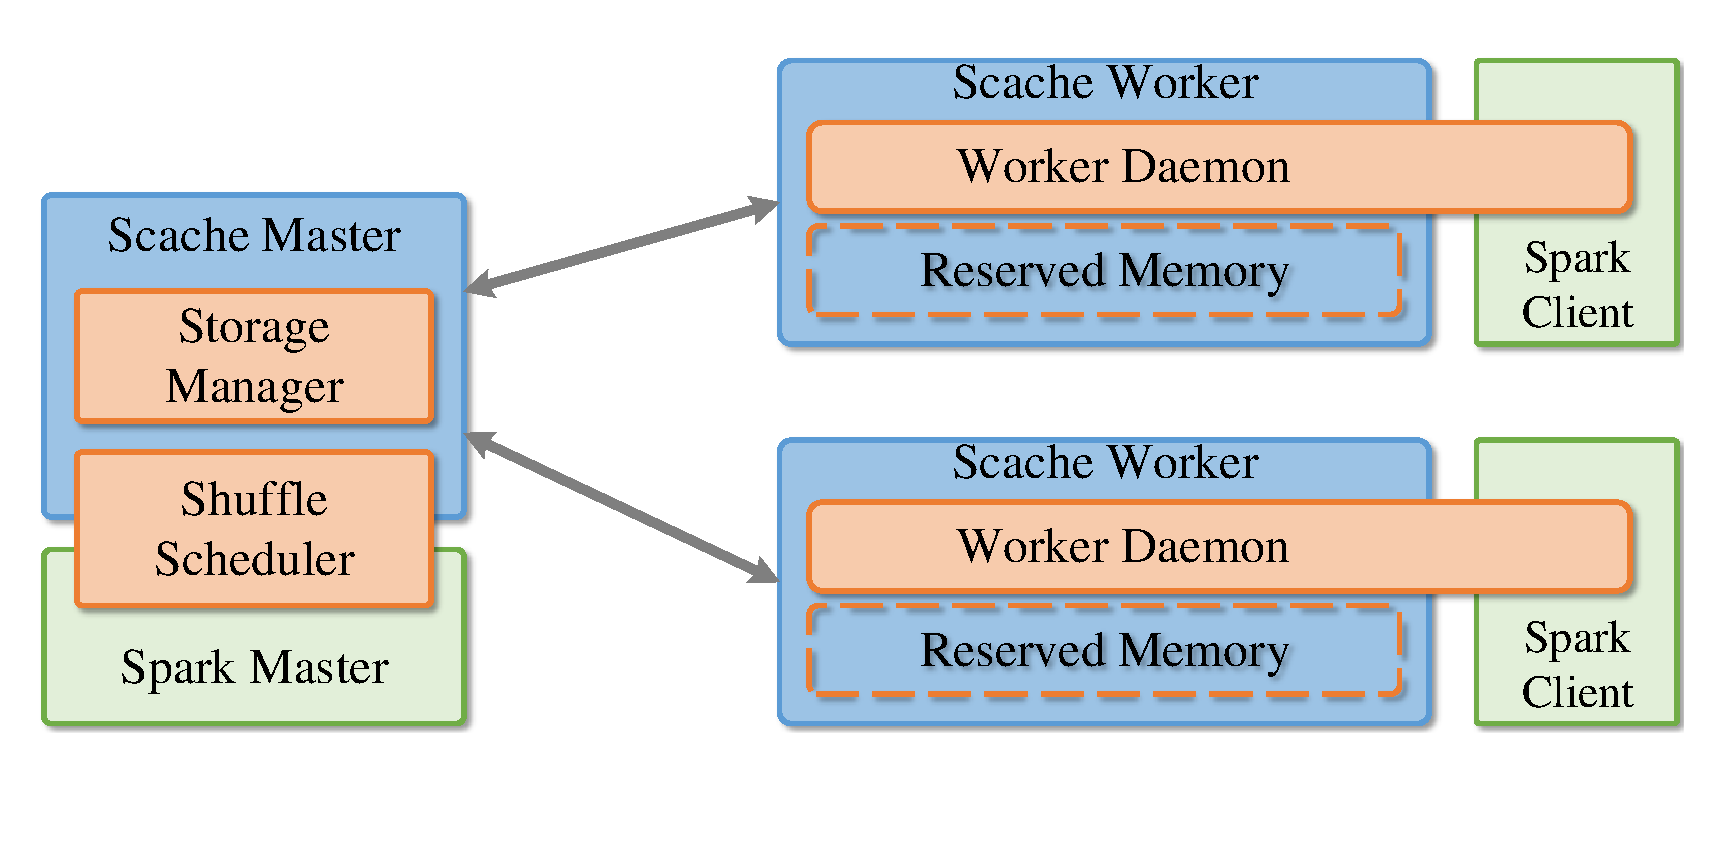
\includegraphics[width=0.8\linewidth]{fig/arch}
% 	\caption{\color{red}SCache Architecture}
% 	\label{fig:arch}
% 	\vspace{-0.5em}
% \end{figure}

\begin{figure}
	\centering
	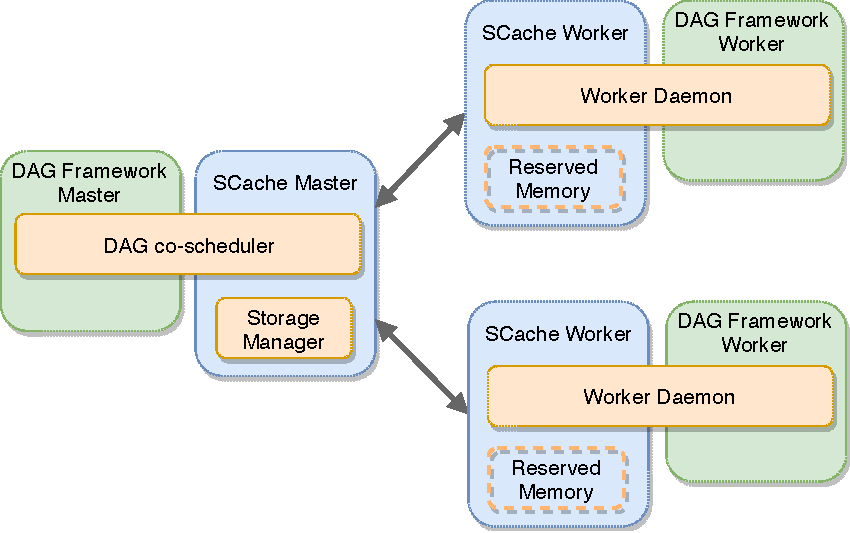
\includegraphics[width=0.8\linewidth]{fig/architecture}
	\caption{\color{blue}SCache Architecture}
	\label{fig:architecture}
	% \vspace{-0.5em}
\end{figure}

\subsection{Memory Management}\label{memorymanage}
As mentioned in Section \ref{observation}, though the shuffle size is relatively small, memory management should still be cautious enough to limit the effect of performance of DAG framework.
When the size of cached blocks reaches the limit of reserved memory, SCache flushes some of them to the disk temporarily, and re-fetches them when some cached shuffle blocks are consumed or pre-fetched. 
To achieve the maximum overall improvement, SCache leverages two constraints to manage the in-memory data-all-or-nothing and context-aware-priority.

\begin{figure}
	\centering
	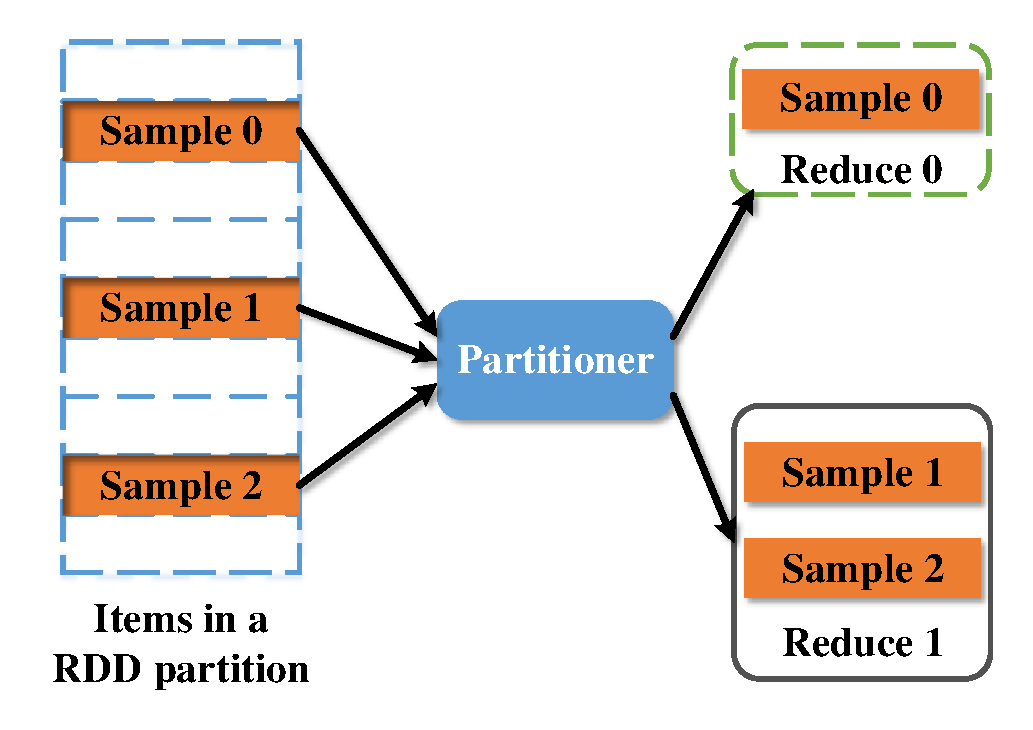
\includegraphics[width=0.6\linewidth]{fig/sample}
	\caption{Reservoir Sampling of One Partition}
	\label{fig:sample}
	\vspace{-1em}
\end{figure}

\subsubsection{All-or-Nothing Constraint}
This acceleration of in-memory cache of a single task is necessary but insufficient for a shorter stage completion time. 
Based on the observation in Section \ref{multi}, in most cases one single stage contains multi-rounds of tasks. 
If one task missed a memory cache and exceeded the original bottleneck of this round, that task might become the new bottleneck and then slow down the whole stage. 
PACMan \cite{pacman} has also proved that for multi-round stage/job, the completion time improves in steps when $n\times number\ of\ tasks\ in\ one\ round$ of tasks have data cached simultaneously. 
Therefore, the cached shuffle blocks need to match the demand of all tasks in one running round at least. We refer to this as the all-or-nothing constraint.

According to all-or-nothing constraint, SCache master leverages the pre-scheduled results to determine the bound of each round, and sets blocks of one round as the minimum unit of storage management.
For those incomplete units, SCache marks them as the lowest priority.
% Following the all-or-noting constraint can maximum the improvement in stage completion time by using reserved memory efficiently.

\subsubsection{Context-Aware-Priority Constraint}
Unlike the traditional cache replacement schemes such as MIN \cite{min}, the cached shuffle data will only be used once (without failure), but the legacy cache managements are designed to improve the hit rate.
SCache leverages application context to select victim storage units when the reserved memory is full.

At first, SCache flushes blocks of the incomplete units to disk cluster-widely.
If all the units are completed, SCache selects victims based on two factors-\textit{inter-shuffle} and \textit{intra-shuffle}.
\begin{itemize}[noitemsep]
	\item Inter-shuffle: SCache master follows the scheduling scheme of Spark to determine the inter-shuffle priority. 
	For example, Spark FIFO scheduler schedules the tasks of different stages according to the submission order. 
	So SCache sets the priorities according to the submission time of each shuffle.
	% For a FAIR scheduler, Spark balances the resource among task sets, which leads to a higher priority for those having more tasks unfinished. 
	% So SCache sets priorities from high to low in a descending order of remaining storage units of a shuffle. 
	% For a FIFO scheduler, Spark schedules the task set that is submitted first. 
	% So SCache sets the priorities according to the submit time of each shuffle unit.
	\item Intra-shuffle: The intra-shuffle priorities are determined according to the task scheduling inside a stage.
	For example Spark schedules tasks with smaller ID at first. 
	Based on this, SCache can assign the lower priority to storage units with a larger task ID.
\end{itemize}

% {\color{red}
% \subsection{Cost of adapting DAG frameworks}
% SCache provides API through RPC, such as \textit{putBlock(blockId)}, \textit{getBlock(blockId)}, and \textit{getScheduleResult(shuffleId)}. The concise design makes it easy to adapt DAG frameworks to enable SCache optimization. For example, it only takes about 500 lines of code in Spark to integrate SCache. By a glance of Hadoop source code, we believe that the costs of enabling SCache on MapReduce \cite{hadoop} and YARN \cite{yarn} based DAG computing framework, such as Tez \cite{tez}, are also very low.
% }
{\color{blue}
\subsection{Analysis of cross-framework capability}\label{crossframework}
Shuffle optimization of SCache inevitably requires modification on DAG frameworks. SCache provides APIs through RPC, such as \textit{putBlock (blockId)}, \textit{getBlock (blockId)}, and \textit{getScheduleResult (shuffleId)}. In order to use SCache, we mainly need to modify two parts of the frameworks: (a) We need to modify codes in the DAG scheduler to let framework provide DAG information and follow the pre-scheduled result of SCache. (b) The shuffle data between the map task and the reduce task should be transferred to SCahce Storge Management.

To prove the cross-framework capability of SCache, we adapt SCache on Hadoop MapReduce and Spark respectively. Taking Hadoop MapReduce as an example, we modify codes in ResourceManager, MapTask and ReduceTask to call SCache APIs through RPC. It takes about 400 lines of code. In Spark, we mainly modify DAGScheduler and the corresponding data fetcher. 
It only takes about 500 lines of code. Such hundreds of lines of code modification are very small compared to the hundreds of thousands of lines of code in DAG framework. We believe that the costs of enabling SCache on other DAG computing frameworks, such as Tez \cite{tez}, are also very low.
}

\subsection{Fault tolerance}\label{fault}
Due to the characteristic of shuffle data (e.g., short-lived, write-once, read-once), we believe fault tolerance is not a crucial goal of SCache at present. 
We plan to implement SCache master with Apache ZooKeeper \cite{zookeeper} to provide constantly service. 
If a failure happened inside the SCache worker, SCache daemon could block the shuffle write/read operations until the worker process restarted without violating the correctness of DAG computing.
A possible way to handle this failure is selecting some backup nodes to store replications. 
But the replications can introduce a significant network overhead \cite{availability}.  
Currently, we left the sever faults (e.g., the failure of a node) to the DAG frameworks. 
We believe it is a more promising way because most DAG frameworks have more advanced fast recovery schemes on the application layer, such as paralleled recovery of Spark. 
Meanwhile, SCache can still provide shuffle optimization during the recovery.





% \subsubsection{Fault Tolerance}
% To prevent the machine failure in cluster leading to inconsistency SCache, the master node will log the meta data of shuffle register and scheduling on the disk. Since we remove the shuffle transfer from the critical path of DAG computing, the disk log will not introduce extra overhead to the DAG framworks. Note that the master can be implemented with Apache ZooKeeper \cite{zookeeper} to provide constantly service to DAG framework.
% At the same time, every work node will send a heartbeat to master to report status. If a failure of work node is detected, the master will the do a simple re-schedule. For those scheduled shuffle units, the master assgins the tasks to other workers with more lightweight workload evenly. Then the new assigned worker will fetch the data again. For the incomplete in memory map blocks on the failure node, SCache simply ignore them since DAG framework will schedule the failure map tasks on another node.

{\color{blue}
\section{Framework Resources Quantification Model}\label{model}

\begin{figure*}
    \centering
	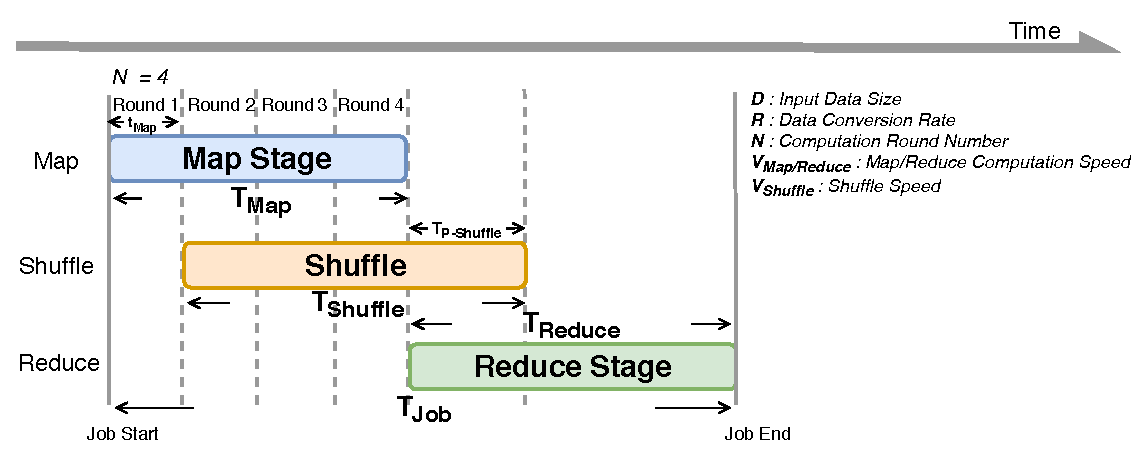
\includegraphics[width=0.85\textwidth]{fig/model_basic}
	\caption{\color{blue}Framework Resources Quantification (FRQ) Model with Full Parallel MapReduce}
    \label{fig:model_basic}
    \vspace{-1em}
\end{figure*}

In this chapter, we introduce \textit{Framework Resources Quantification} (FRQ) model to describe the performance of DAG frameworks.
FRQ model quantifies computing and I/O resources and displays them in time dimension. According to FRQ model, we can calculate the execution time required by the application under any circumstances, including different DAG framework, hardware environment, and so on. Therefore FRQ model is able to help us analyze the resources scheduling of DAG framework and evaluate their performance. We will first introduce FRQ model in Subsection \ref{model_overview}. In the following Subsection \ref{model_analysis}, we will use FRQ model to describe three different computation job and analyze their performance. In the last Subsection \ref{model_verification}, we will use the actual experimental results to verify the FRQ model.

\subsection{The FRQ Model}\label{model_overview}
The current distributed data parallel computing frameworks mostly use \textit{Directed acyclic graphs} (DAGs) to describe computation logic. A shuffle phase is required between each adjacent DAG computation phase. In order to better analyze the relationship between the computation phase and the shuffle phase, we propose FRQ model. After quantifying computing and I/O resources, FRQ model is able to describe different resource scheduling strategies. For convenience, we introduce FRQ model by taking a simple MapReduce job as an example in this section.

Figure \ref{fig:model_basic} shows how the FRQ model describes a MapReduce task. FRQ model has five input parameters:
\begin{itemize}
	\item Input Data Size \((D)\): The data size of the computation phase.
	\item Data Conversion Rate \((R)\): The conversion rate of the input data to the shuffle data during a computation phase. This conversion rate depends on the algorithm used in the computation phase.
    \item Computation Round Number \((N)\): The number of rounds needed to complete the computation phase using the current computation resources. The number of rounds depends on the current computation resources and the settings of the computation job. Take Hadoop MapReduce as an example, suppose we have 50 CPUs and enough memory, the map phase consists of 200 map tasks. Then we need 4 rounds of computation to complete the map phase.
    \item Computation Speed \((V_{i})\): 
    The computation speed for each computation phase. The computation speed depends on the algorithm used in the computation phase.
    \item Shuffle Speed \((V_{Shuffle})\): 
    Transmission speed during shuffle. Shuffle speed depends on Network and storage device bandwidth.
\end{itemize}

We can calculate the execution time of each phase of the job with these five parameters. As shown in Figure \ref{fig:model_basic}, in full parallel mapReduce, the total execution time of a job is the sum of the map phase time and reduce phase time:
\begin{equation}
\label{equation_Tjob}
\begin{aligned}
    T_{Job} &= T_{Map} + T_{Reduce}
\end{aligned}
\end{equation}
map phase time depends on input data size and Map computation speed:
\begin{equation}
\label{equation_Tmap}
\begin{aligned}
    T_{Map} &= {{\frac{D}{V_{Map}}}}
\end{aligned}
\end{equation}
The reduce phase time formula is as follows:
\begin{equation}
\label{equation_Treduce}
\begin{aligned}
    T_{Reduce} &= \frac{D \times R}{V_{Reduce}} + K \times T_{P\_Shuffle}
\end{aligned}
\end{equation}

We use \(T_{P\_Shuffle}\) to represent the overlap time between shuffle phase and reduce phase. \(T_{Shuffle}\) represents the total time of shuffle phase. 
The relationship between \(T_{P\_Shuffle}\) and \(T_{Shuffle}\) is determined by the resources scheduling strategy of DAG frameworks. This relationship will be shown in the following Subsection \ref{model_analysis}.  
\(\frac{D \times R}{V_{Reduce}}\) represents the ideal computation time of a reduce phase, and \(K \times T_{P\_Shuffle}\) represents the computing overhead. \(K\) is an empirical value. 
Because the computation of the reduce phase relies on the data transfer results of the shuffle phase, a portion of the computation in the reduce phase need to wait for the transfer results. The overhead is caused by these waiting. The FRQ model uses K to indicate the extent of the waiting.

\begin{equation}
\label{equation_Tshuffle}
\begin{aligned}
    T_{Shuffle} &= {{\frac{D}{V_{Shuffle}}}}
\end{aligned}
\end{equation}

For shuffle-heavy computing jobs, we can optimize the job completion time by reducing \(T_{P\_Shuffle}\). Improving I/O speed is a effective way to reduce shuffle time. Another optimization method is to use the idle I/O resources in the map phase for pre-fetching (see Figure \ref{fig:model_basic}). Both of the above methods can effectively reduce \(T_{P\_Shuffle}\). When using FRQ model to describe a computation job, we can easily analyze the resource scheduling strategy of the computation framework. Different computing frameworks may use different resource scheduling strategies. FRQ model can evaluate the scheduling strategies of these computing frameworks and help us optimize them.

\subsection{Model Analysis}\label{model_analysis}

\begin{figure}
	\centering
	\begin{minipage}[hb]{\linewidth}
		\begin{subfigure}{\linewidth}
			\begin{minipage}{\linewidth}
				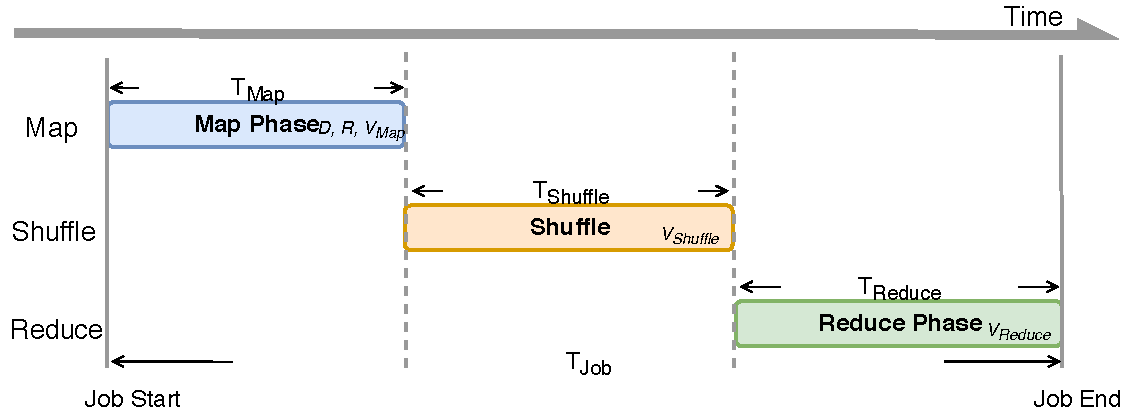
\includegraphics[width=\linewidth]{fig/model_original}
				\caption{\color{blue}Full Serial MapReduce}
				\label{fig:model_original}
			\end{minipage}
			\begin{minipage}{\linewidth}
				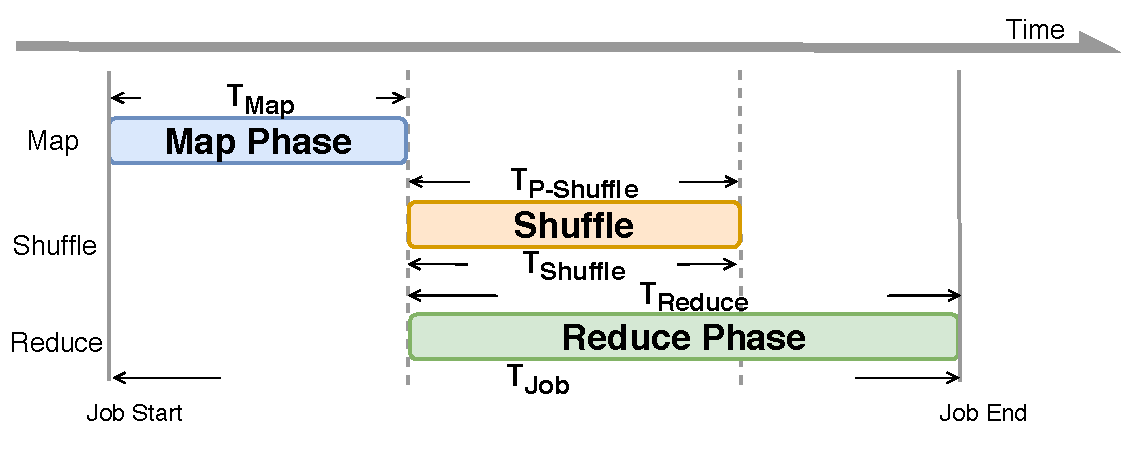
\includegraphics[width=\linewidth]{fig/model_hadoop}
				\caption{\color{blue}Half Parallel MapReduce}
				\label{fig:model_hadoop}
			\end{minipage}
		\end{subfigure}
		\caption{\color{blue}Framework Resources Quantification (FRQ) Model with Different Scheduling Strategies}
		\label{fig:model_strategies}
	\end{minipage}
\end{figure}

The FRQ model can describe a variety of resource scheduling strategies. First, we analyze a naive scheduling strategy. As shown in Figure \ref{fig:model_original}, FRQ model describes a MapReduce job that is fully serially executed. The overlap time between shuffle phase and the reduce phase is \(0\), in which case \(T_{P\_Shuffle}\) is \(0\). Therefore, the overhead of the reduce phase is 0. But since shuffle and computation are serial execution, the total execution time of a job is different from the above:
\begin{equation}
\label{equation_Tjob2}
\begin{aligned}
    T_{Job} &= T_{Map} + T_{Shuffle} + T_{Reduce}
\end{aligned}
\end{equation}
Apache Spark uses this scheduling strategy by default. Due to serialization, the I/O resource is idle during the reduce phase and map phase. The scheduling strategy is simple and has a lot of room for optimization.

Figure \ref{fig:model_hadoop} shows one of the optimization methods. In this scheduling strategy, shuffle phase and reduce phase start at the same time. In this case, \(T_{P\_Shuffle}\) is equal to \(T_{Shuffle}\). Due to the increase in \(T_{P\_Shuffle}\), the time of reduce phase will increase (according to equation \ref{equation_Treduce}). Because the shuffle phase and the computation phase are executed in parallel, the total execution time of job is the sum of \(T_{Map}\) and \(T_{Reduce}\) (see equation \ref{equation_Tjob}). The execution time of shuffle phase is hidden in the reduce phase. This scheduling strategy is used by Hadoop MapReduce. After analyzing this model, we believe that this strategy will be more efficient than the above serial strategy in the same situation. Meanwhile, we found that the I/O resource in the map phase is still idle. This scheduling strategy can be optimized.

\begin{figure}
	\centering
	\begin{minipage}[hb]{\linewidth}
		\begin{subfigure}{\linewidth}
			\begin{minipage}{\linewidth}
				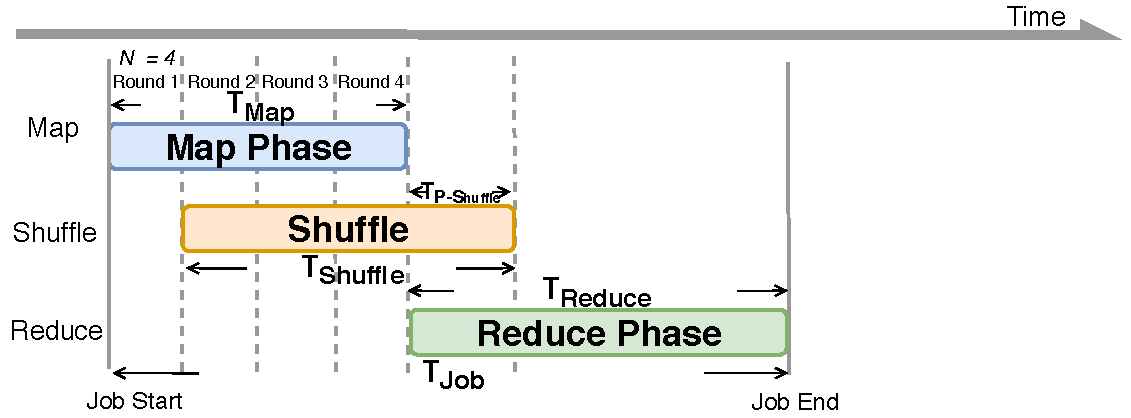
\includegraphics[width=\linewidth]{fig/model_scache1}
				\caption{\color{blue}If \(V_{Map} \times R \ge V_{Shuffle}\)}
				\label{fig:model_scache1}
			\end{minipage}
			\begin{minipage}{\linewidth}
				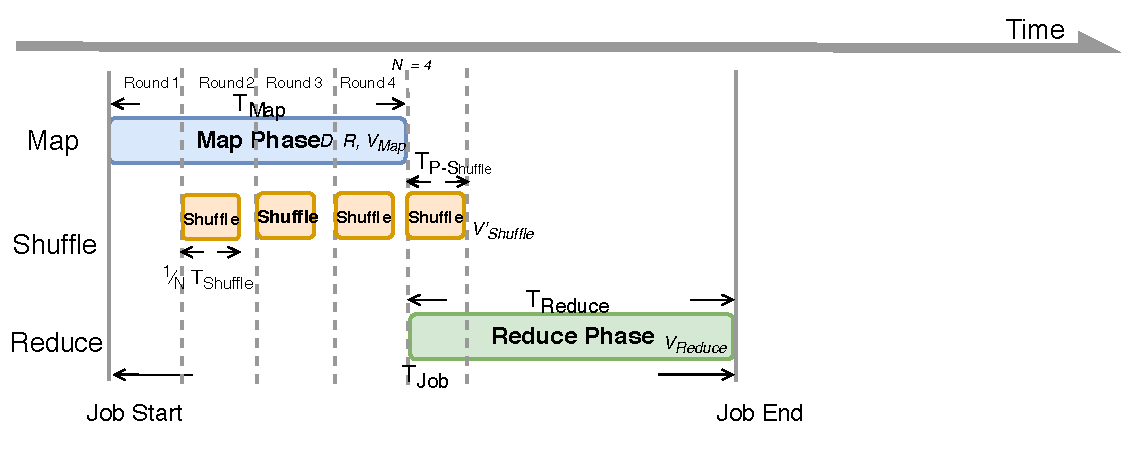
\includegraphics[width=\linewidth]{fig/model_scache2}
				\caption{\color{blue}If \(V_{Map} \times R < V_{Shuffle}\)}
				\label{fig:model_scache2}
			\end{minipage}
		\end{subfigure}
		\caption{\color{blue}Framework Resources Quantification (FRQ) Model with Full Parallel MapReduce in Different Environments}
		\label{fig:model_scache}
	\end{minipage}
\end{figure}

Hadoop MapReduce overlaps shuffle phase with reduce phase and utilizes idle resources. We intuitively think that we can also overlap shuffle phase one and map phases. We implemented this idea with SCache.
Figure \ref{fig:model_scache} shows the scheduling strategy for Hadoop MapReduce with SCache (Suppose N is 4). SCache starts pre-fetching and pre-scheduling in the map phase. This scheduling strategy can make better use of resources and avoid the I/O resource being idle in the map phase. According to the design of SCache pre-fetching, we found that using FRQ model to describe the scheduling strategy of SCache needs to distinguish two situations:

\begin{enumerate}
    \item 
    \(V_{Map} \times R \ge V_{Shuffle}\) (Figure \ref{fig:model_scache1}): 
	The meaning of \(V_{Map} \times R\) is the speed at which shuffle data is generated. The meaning of the inequality is that the speed of generating shuffle data(\(V_{Map} \times R\)) is greater than or equal to the shuffle speed(\(V_{Shuffle}\)). When the Round1 of the map phase ends, the SCache starts shuffling data until the end of the shuffle phase. Due to shuffle speed is slower, the shuffle phase is uninterrupted. SCache transmit the shuffle data generated in the last round of map phase during the reduce phase. Therefore \(T_{PShuffle}\) is equal to one-\(N\) of the total time of the shuffle phase:
	\begin{equation}
		\label{equation_Tpshuffle1}
		\begin{aligned}
			T_{P\_Shuffle} &= T_{Shuffle} - \frac{(N - 1)\times T_{Map}}{N}
		\end{aligned}
	\end{equation}
	
    \item \(V_{Map} \times R < V_{Shuffle}\) (Figure \ref{fig:model_scache2}): 
	When the speed of generating shuffle data (\(V_{Map} \times R\)) is less than the shuffle speed (\(V_{Shuffle}\)), SCache needs to wait for shuffle data to be generated. As Figure \ref{fig:model_scache2} shown, the shuffle phase will be interrupted in each Round. Thus \(T_{P_Shuffle}\) is equal to the total time of shuffle (\(T_{Shuffle}\)) minus the time that shuffle is executed in the map phase:
	\begin{equation}
		\label{equation_Tpshuffle2}
		\begin{aligned}
			T_{P\_Shuffle} &= T_{Shuffle} \times \frac{1}{N}
		\end{aligned}
	\end{equation}
\end{enumerate}

% After analyzing the above two situations, we figure out the formula for \(T_{P\_Shuffle}\):
% \begin{equation}
%     \label{equation_Tpshuffle}
%     \begin{aligned}
%     T_{P\_Shuffle} &=
%         \begin{cases} 
%         T_{Shuffle} - \frac{(N - 1)\times T_{Map}}{N} & , V_{Map} \times R \ge V_{Shuffle} \\ 
%         T_{Shuffle} \times \frac{1}{N} & , V_{Map} \times R < V_{Shuffle}
%         \end{cases}
%     \end{aligned}
% \end{equation}
% If the shuffle speed is slow(\(V_{Map} \times R \ge V_{Shuffle}\)), SCache transmit the shuffle data generated in the last round of map phase during the reduce phase. Therefore \(T_{PShuffle}\) is equal to one-\(N\) of the total time of the shuffle phase.

% If the shuffle speed is fast (\(V_{Map} \times R < V_{Shuffle}\)), \(T_{P_Shuffle}\) is equal to the total time of shuffle (\(T_{Shuffle}\)) minus the time that shuffle is executed in the map phase.

Compared to the original Hadoop MapReduce resource scheduling strategy, Hadoop MapReduce with SCache reduces \(T_{P\_Shuffle}\) and thus lessens \(T_{Reduce}\). This is how pre-fetching optimizes the total execution time of a job.


\begin{table*}[!t]
\renewcommand{\arraystretch}{1.3}
\caption{\color{blue}Hadoop MapReduce on 4 nodes cluster in FRQ model}
\label{table1}
\centering
\(D\): GB, \(V_{i}\): GB/s, \(T_{i}\): s
\begin{tabular}{|c||c|c|c|c|c|c|c||c|c|c|c|c|c|c|}
\hline
 &
\(D\) &	
\(R\) &	
\(N\) &	
\(V_{Map}\) &	
\(V_{Reduce}\) &	
\(V_{Shuffle}\) &	
\(K\) &	
\(T_{Map}\) &	
\(T_{Shuffle}\) &	
\(T_{P\_Shuffle}\) &
\(T_{Reduce}\) & 
\(T_{Job}\) & 
\(Exp T_{Job}\) &
\(Error\)\\

\hline
 & 16	& 1	& 2 &	0.65 &	1 &	0.47 &	0.5 &	24.62 &		34.04	 &	21.73 &	26.87 &	51.48	& 55  &		6.39\% \\
 SCache
 & 32	& 1	& 4 &	0.65 &	1 &	0.47 &	0.5 &	49.23 &		68.09	 &	31.16 &	47.58 &	96.81	& 104 & 	6.91\% \\
 & 48	& 1	& 6 &	0.65 &	1 &	0.47 &	0.5 &	73.85 &		102.13 &	40.59 &	68.29 &	142.14	& 151 & 	5.87\% \\
 & 64	& 1	& 8 &	0.65 &	1 &	0.47 &	0.5 &	98.46 &		136.17 &	50.02 &	89.01 &	187.47	& 193 & 	2.87\% \\
 \hline
 & 16	& 1 & 2 &	0.65 &	1 &	0.47 &	0.6 &	24.62 &		34.04	&	34.04	&	36.43	&	61.04	&	73	&	16.38\%	\\
 Legacy
 & 32	& 1 & 4 &	0.65 &	1 &	0.47 &	0.6 &	49.23 &		68.09	&	68.09	&	72.85	&	122.08	&	135	&	9.57\%	\\
 & 48	& 1 & 6 &	0.65 &	1 &	0.47 &	0.6 &	73.85 &		102.13	&	102.13	&	109.28	&	183.12	&	188	&	2.59\%	\\
 & 64	& 1 & 8 &	0.65 &	1 &	0.47 &	0.6 &	98.46 &		136.17	&	136.17	&	145.70	&	244.16	&	249	&	1.94\%	\\
\hline
\end{tabular}
\end{table*}
% \subsection{Performance Analysis}\label{model_performance_analysis}

\begin{table*}[!t]

\renewcommand{\arraystretch}{1.3}
\caption{\color{blue}Hadoop MapReduce on 50 AWS m4.xlarge nodes cluster in FRQ model}
\label{table2}
\centering
\(D\): GB, \(V_{i}\): GB/s, \(T_{i}\): s
\begin{tabular}{|c||c|c|c|c|c|c|c||c|c|c|c|c|c|c|}
\hline
 &
\(D\) &	
\(R\) &	
\(N\) &	
\(V_{Map}\) &	
\(V_{Reduce}\) &	
\(V_{Shuffle}\) &	
\(K\) &	
\(T_{Map}\) &	
\(T_{Shuffle}\) &	
\(T_{P\_Shuffle}\) &
\(T_{Reduce}\) & 
\(T_{Job}\) & 
\(Exp T_{Job}\) &
\(Error\)\\

\hline
& 128	& 1 & 5 &	1.15 &	1.46	&	1.4 &	0.5 &	111.30 &	91.43	&	18.29	&	96.81	&	208.12	&	232	&	10.29\%	\\
SCache
& 256	& 1 & 5 &	1.15 &	1.46	&	1.4 &	0.5 &	222.61 &	182.86	&	36.57	&	193.63	&	416.24	&	432	&	3.65\%	\\
& 384	& 1 & 5 &	1.15 &	1.46	&	1.4 &	0.5 &	333.91 &	274.29	&	54.86	&	290.44	&	624.36	&	685 &	8.85\%	\\
% & 512	& 1 & 5 &	1.15 &	1.46	&	1.4 &	0.5 &	445.22 &	365.71	&	91.43	&			&	841.62	&	1135 &	25.85\%	\\
\hline
& 128	& 1 & 5 &	1.15 &	1.46	&	1.4 &	0.6 &	111.30 &	91.43	&	91.43	&	142.53	&	253.83	&	266 &	4.57\%	\\
Legacy
& 256	& 1 & 5 &	1.15 &	1.46	&	1.4 &	0.6 &	222.61 &	182.86	&	182.86	&	285.06	&	507.67	&	524 &	3.12\%	\\
& 384	& 1 & 5 &	1.15 &	1.46	&	1.4 &	0.6 &	333.91 &	274.29	&	274.29	&	427.59	&	761.50	&	776 &	1.87\%	\\
% & 512	& 1 & 5 &	1.15 &	1.46	&	1.4 &	0.6 &	445.22 &	365.71	&	365.71	&	588.40	&	1033.62	&	1312 &	21.22\%	\\

\hline
\end{tabular}
\end{table*}

\subsection{Model Verification}\label{model_verification}
In order to verify FRQ model, we run experiment on two environments. The first environment is on Amazon EC2 and it has 50 m4.xlarge nodes as shown in Section \ref{stepup}. Another environment is in our lab. Out lab environment has 4 nodes and each nodes has 128GB and 32 CPUs. To simplify the calculation of the FRQ model, we use Hadoop MapReduce as framework and Terasort as experimental application. We deployed Hadoop with SCache and without SCache on both environments.

Table \ref{table1} shows the calculational results of FRQ model in the lab environment. Workload is from 16 GB to 64 GB. \(D\) and \(N\) are set according to the application parameters. \(R, V_{Map}, V_{Shuffle},\)and \(V_{Reduce}\) are calculated based on experimental results. K is the empirical value, we set \(K\) to 0.5 and 0.6, which reflects that \(T_{P\_Shuffle}\) has less impact on the reduce phase in the case of SCache. The formulas of \(T_{Job}, T_{Map}, T_{Reduce}\) and \(T_{Shuffle}\) are Equation \ref{equation_Tjob}, Equation \ref{equation_Tmap}, Equation \ref{equation_Treduce} and Equation \ref{equation_Tshuffle}, respectively. In the case of SCache, Terasort on Hadoop MapReduce satisfies the situation in Figure \ref{fig:model_scache1} (\(V_{Map} \times R \ge V_{Shuffle}\)), thus the formula of \(T_{P\_Shuffle}\) is Equation \ref{equation_Tpshuffle1}. In the case of Legacy, since pre-fetching is not used, \(T_{P\_Shuffle}\) is equal to \(T_{Shuffle}\)(see Equation \ref{equation_Tshuffle}). \(ExpT_{Job}\) represents the actual experiment data, we calculate \(Error\) according to \(T_{Job}\) and \(ExpT_{Job}\). The formula of \(Error\) is:
\begin{equation}
	\label{equation_error}
	\begin{aligned}
		Error &= \frac{ExpT_{Job} - T_{Job}}{T_{Job}}
	\end{aligned}
\end{equation}

Table \ref{table2} shows the calculational results of FRQ model in Amazon EC2 environment. \(V_{Map}, V_{Shuffle},\) and \(V_{Reduce}\) are modified because of the different hardware devices. We also set K to the same empirical value. The formulas in the table are all the same except \(T_{P\_Shuffle}\). In this environment, Terasort on Hadoop MapReduce satisfies the situation in Figure \ref{fig:model_scache2}(\(V_{Map} \times R < V_{Shuffle}\)), thus the formula of \(T_{P\_Shuffle}\) is Equation \ref{equation_Tpshuffle2}. In the previous case, \(T_{P\_Shuffle}\) is still euqal to \(T_{Shuffle}\).

\begin{figure}
	\centering
	\begin{minipage}[hb]{\linewidth}
		\begin{subfigure}{\linewidth}
			\begin{minipage}{\linewidth}
				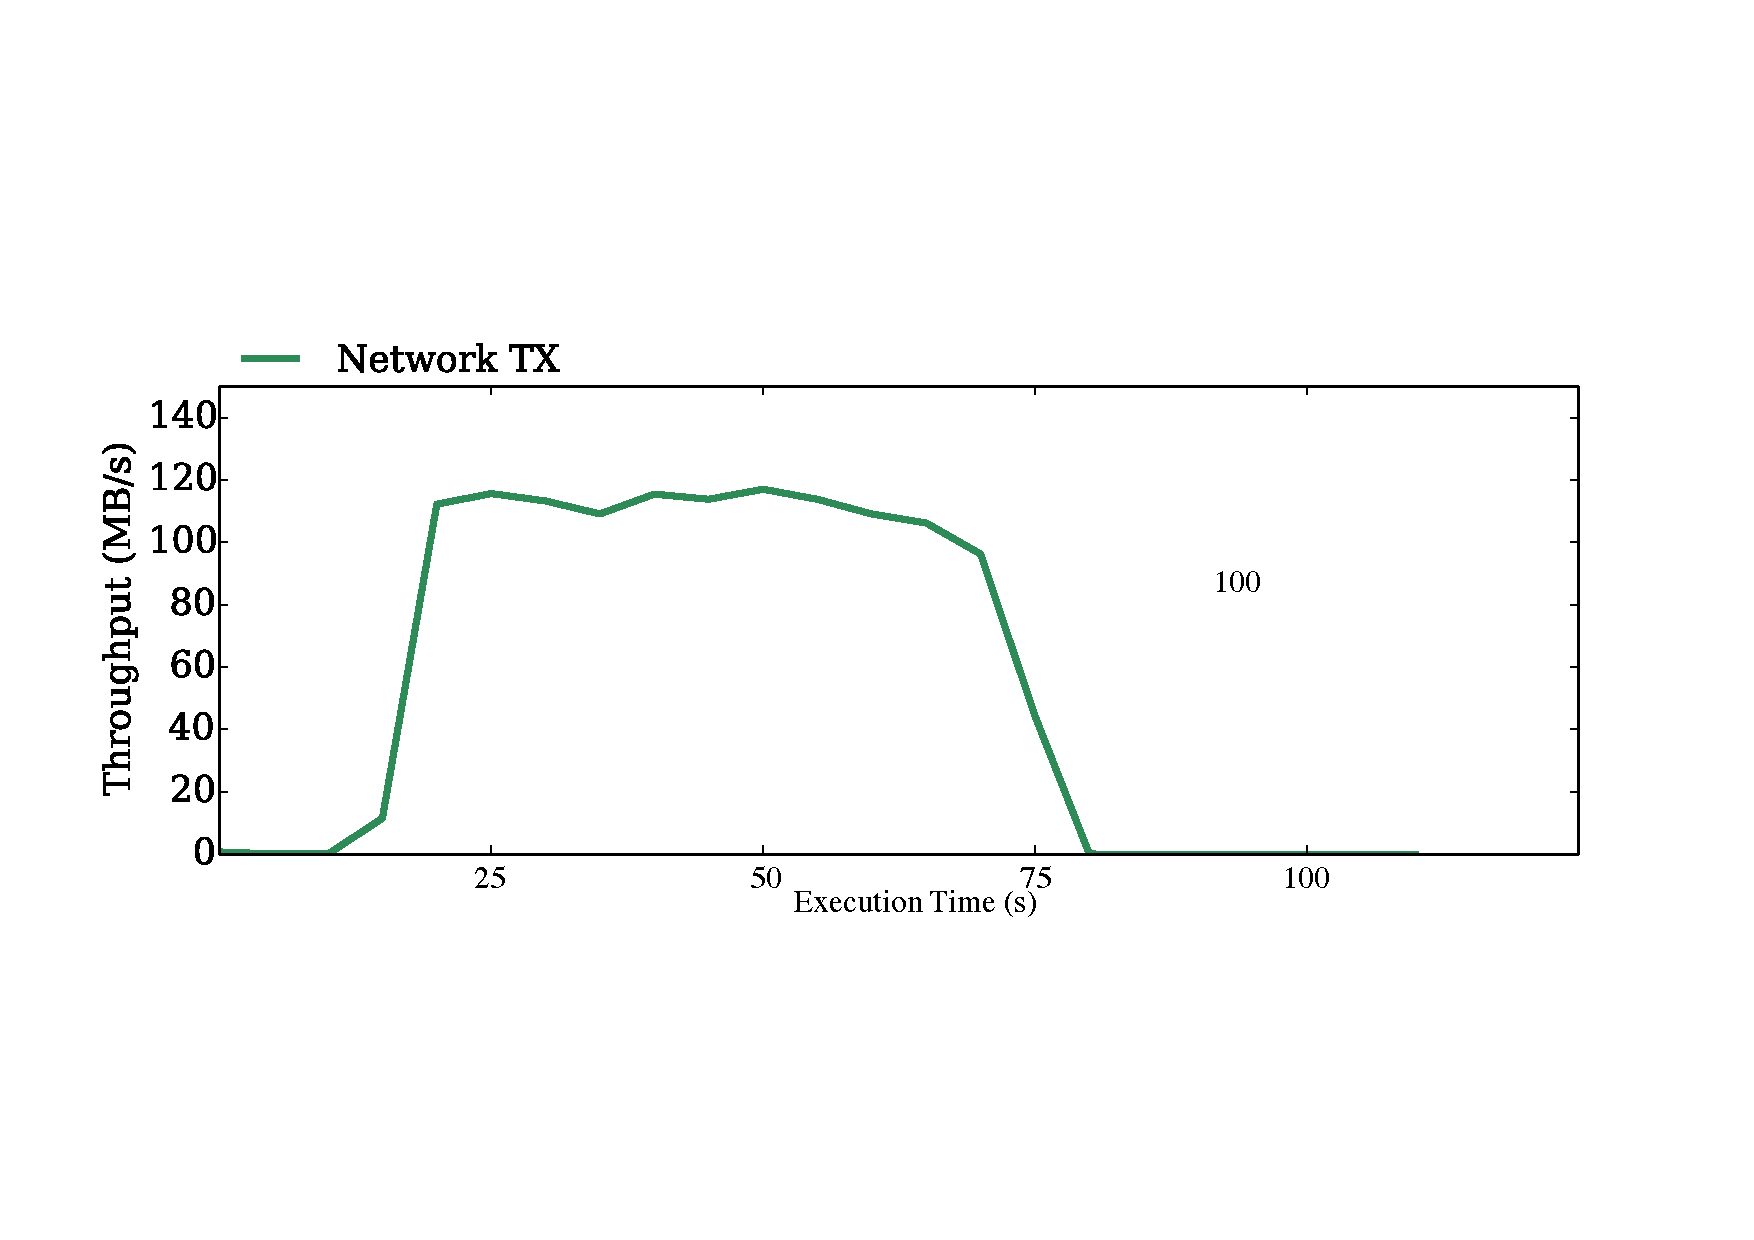
\includegraphics[width=\linewidth]{fig/hadoop_net1}
				\caption{\color{blue}If \(V_{Map} \times R \ge V_{Shuffle}\)}
				\label{fig:hadoop_net1}
			\end{minipage}
			\begin{minipage}{\linewidth}
				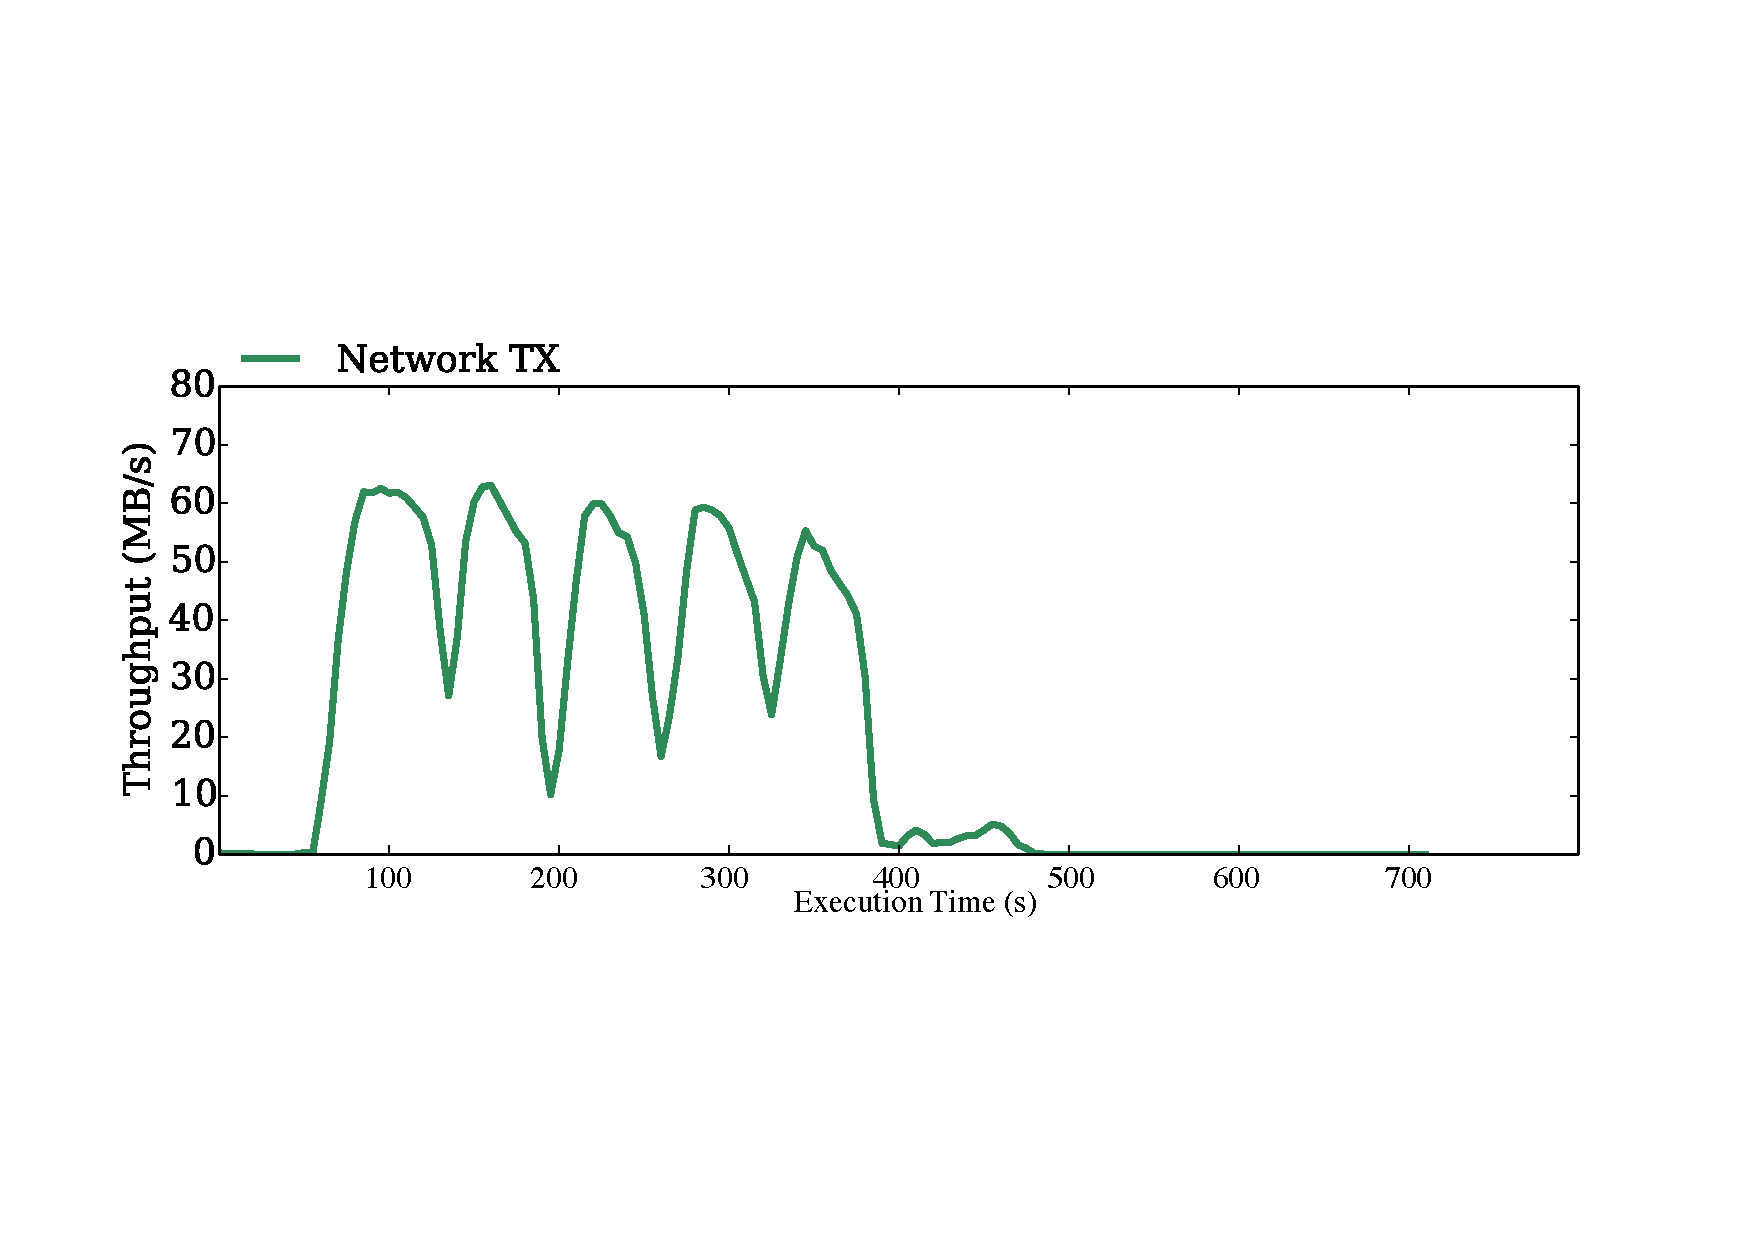
\includegraphics[width=\linewidth]{fig/hadoop_net2}
				\caption{\color{blue}If \(V_{Map} \times R < V_{Shuffle}\)}
				\label{fig:hadoop_net2}
			\end{minipage}
		\end{subfigure}
		\caption{\color{blue}Network utilization on Hadoop MapReduce with SCache}
		\label{fig:hadoop_net}
	\end{minipage}
\end{figure}

In order to verify the above-mentioned two cases when using SCache, we monitor network utilization and plot it in Figure \ref{fig:hadoop_net}. Figure \ref{fig:hadoop_net1} shows the utilization of Terasort in the lab environment. The network utilization remains high until shuffle phase is complete. This situation is consistent with Figure \ref{fig:model_scache1}. Figure \ref{fig:hadoop_net2} shows the utilization in Amazon EC2 environment. 
The network utilization has 5 regular peaks. This situation is also consistent with Figure \ref{fig:model_scache2}. Therefore, we believe that FRQ model is able to accurately describe framework with SCache.

In terms of accuracy, the experimental values are all greater than the calculated values. This is because the application has some extra overhead at runtime, such as network warm-up, the overhead of allocating slots, and so on. In the case where the input data is small and the total time is short, the error caused by the overhead is amplified. Overall, the error between \(T_{Job}\) and \(ExpT_{Job}\) is basically below 10\%, such errors are within tolerance. Therefore, we believe that FRQ model can accurately describe DAG framework.
}
\section{Evaluation}\label{evaluation}
This section reveals the evaluation of SCache with comprehensive workloads and benchmarks. 
First we run a job with single shuffle to analyze hardware utilization and see the impacts of different components from the scope of a task to a job. 
Then we use a recognized shuffle intensive benchmark --- Terasort to evaluate SCache with different data partition schemes.

\begin{figure}
	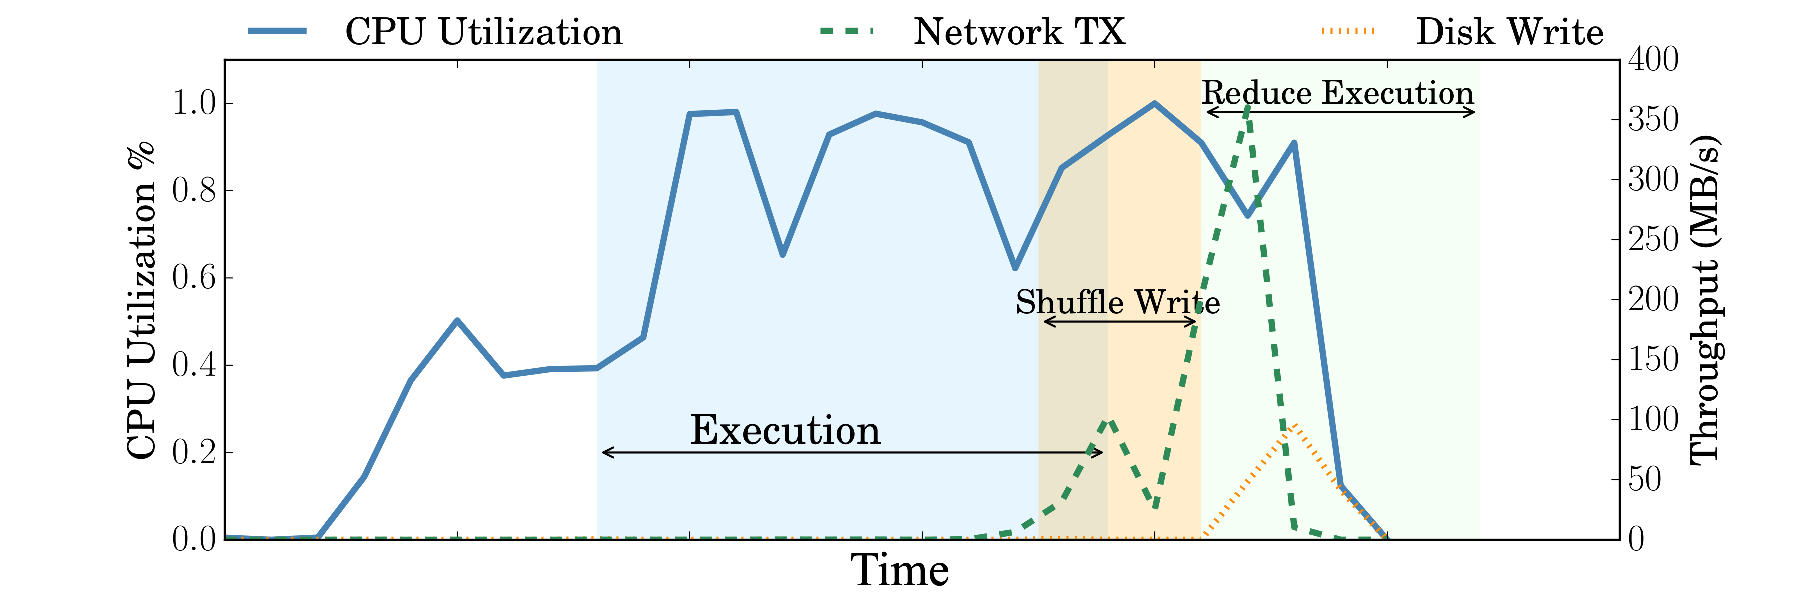
\includegraphics[width=\linewidth]{fig/scache_util}
	\caption{CPU utilization and I/O throughput of a node during a Spark single shuffle application With SCache}
	\label{fig:scache_util}
\end{figure}

In order to prove the performance gain of SCache with a real production workload, we also evaluate Spark TPC-DS\footnote{https://github.com/databricks/spark-sql-perf} and present the overall performance improvement.
{\color{blue}
To prove SCache compatibility as a cross-framework plug-in, we implemented SCache on both Hadoop MapReduce and Spark. 
Due to the simple DAG computing in Hadoop MapReduce, we only use Terasort as a shuffle-heavy benchmark to evaluate the performance of Hadoop MapReduce with SCache.
}
Finally, we measure the overhead of weighted reservoir sampling. 
In summary, SCache can decrease ~$89\%$ time of Spark shuffle without introducing extra network transfer.
More impressively, the overall completion time of TPC-DS can be improved ~$40\%$ on average by applying the optimization from SCache.
{\color{blue}Meanwhile, Hadoop MapReduce with SCache optimize job completion time by up to 15\% and an average of 13\%}

% Because a complex Spark application consists of multiple stages. The completion time of each stage varies under different input data, configurations and different number of stages. This uncertainty leads to the dilemma that dramatic fluctuation occurs in overall performance comparison. To present a straightforward illustration, we limit the scope of most evaluations in a single stage.
\begin{figure*}
	\centering
	\begin{minipage}[t]{.32\linewidth}
		\begin{subfigure}{\linewidth}
			\begin{minipage}{\linewidth}
				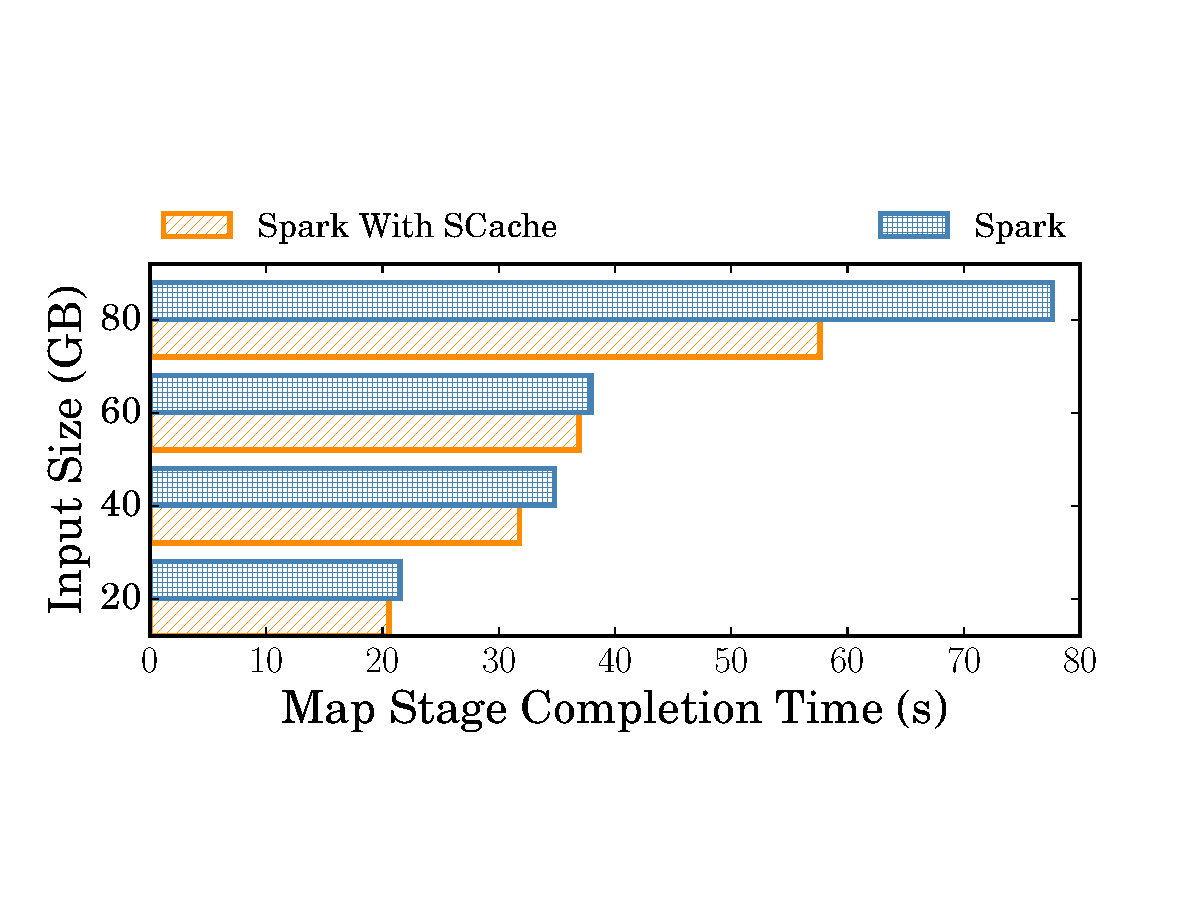
\includegraphics[width=\linewidth]{fig/groupbymapstage}
				\caption{Map Stage Completion Time}
				\label{fig:mapstage}
			\end{minipage}
			\begin{minipage}{\linewidth}
				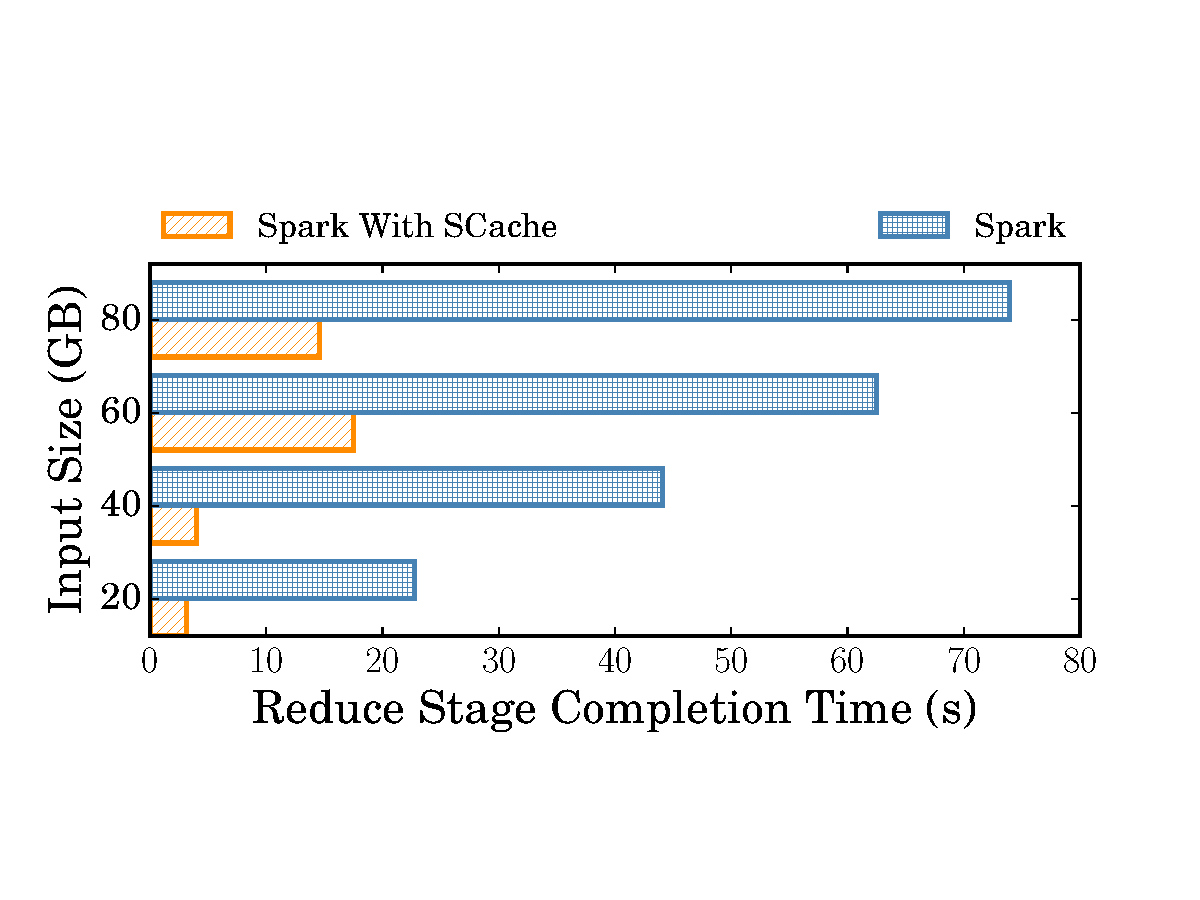
\includegraphics[width=\linewidth]{fig/groupbyreducestage}
				\caption{Reduce Stage Completion Time}
				\label{fig:reducestage}	
			\end{minipage}
		\end{subfigure}
		\caption{Stage Completion Time of Single Shuffle Test}
		\label{fig:singleshuffle}
	\end{minipage}	
	\begin{minipage}[t]{.32\linewidth}
		\begin{subfigure}{\linewidth}
			\begin{minipage}{\linewidth}
				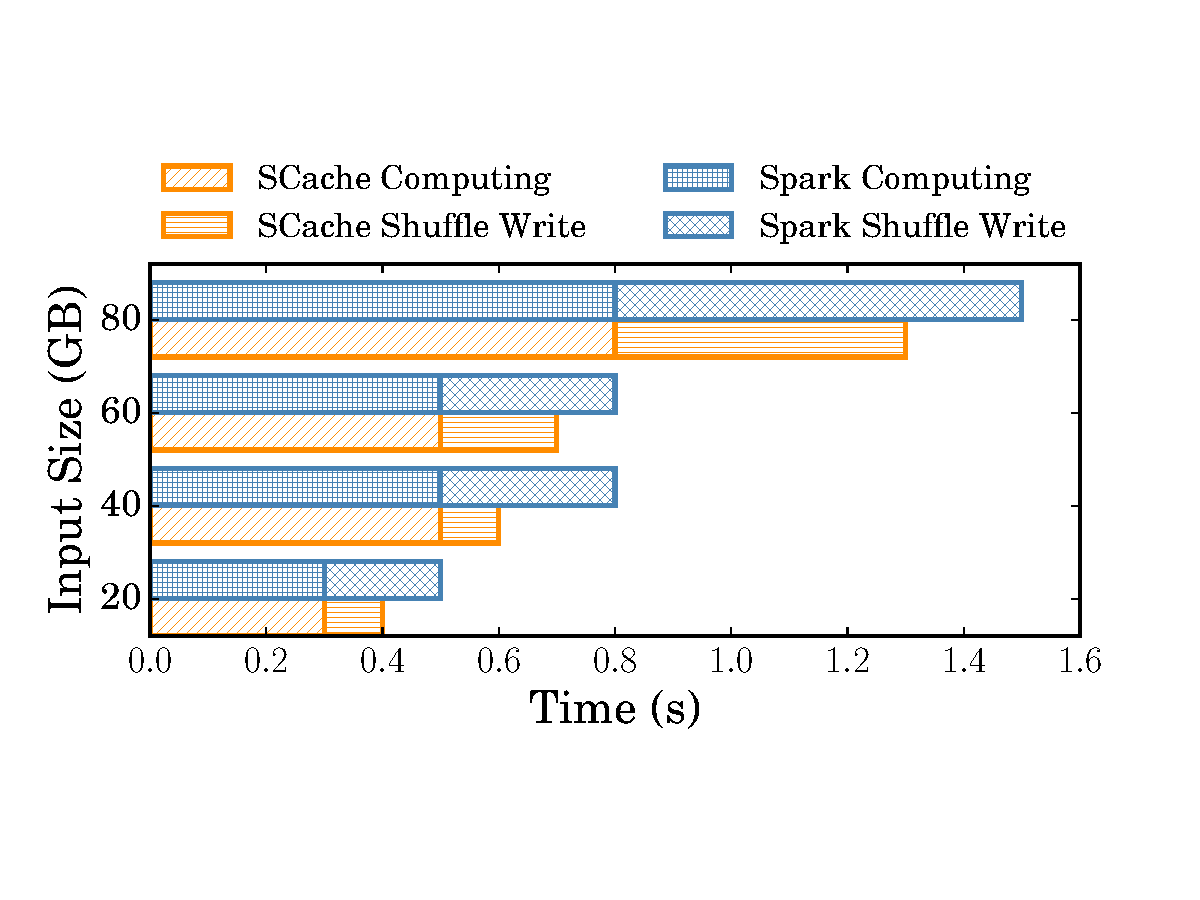
\includegraphics[width=\linewidth]{fig/groupbymaptask}
				\caption{Median Task in Map Stages}
				\label{fig:maptask}
			\end{minipage}

			\begin{minipage}{\linewidth}
				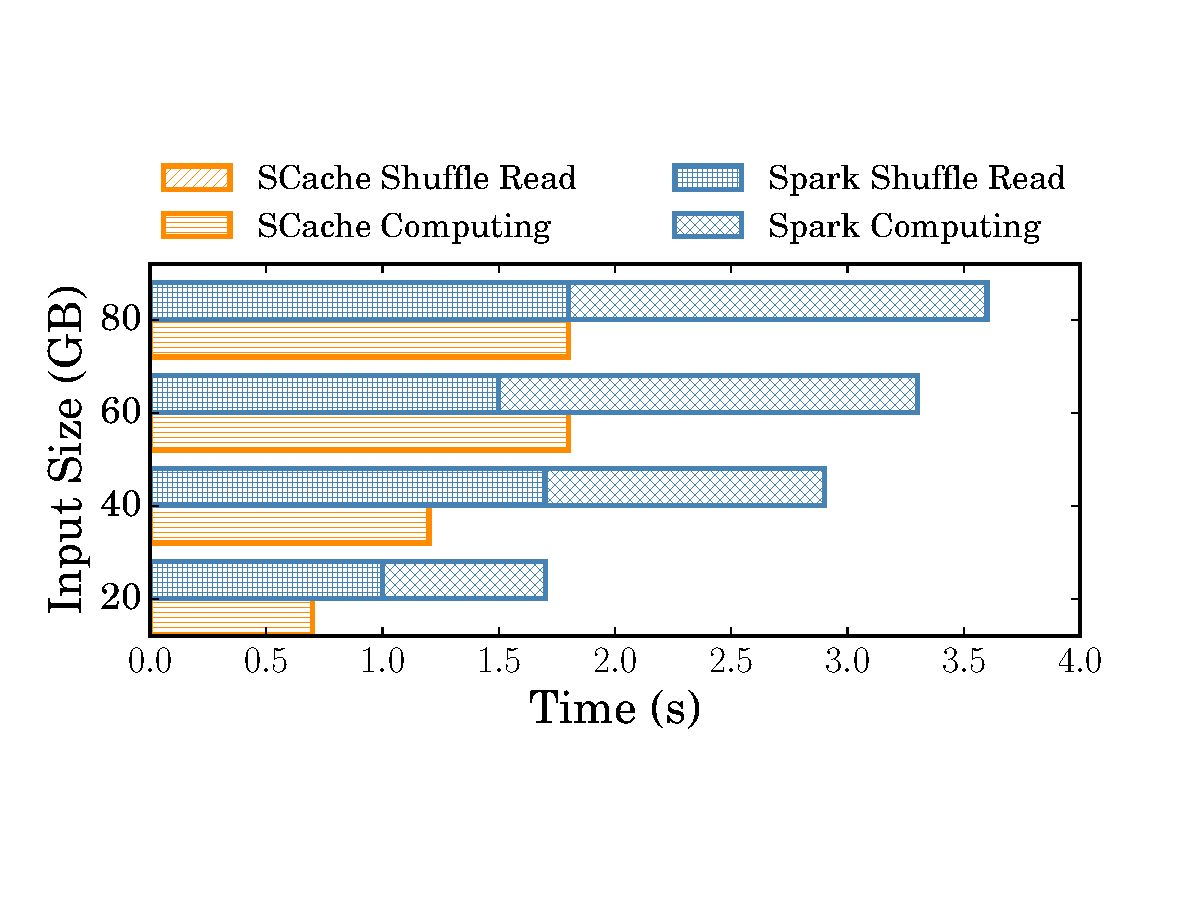
\includegraphics[width=\linewidth]{fig/groupbyreducetask}
				\caption{Median Task in Reduce Stages}
				\label{fig:reducetask}
			\end{minipage}
		\end{subfigure}
		\caption{Median Task Completion Time of Single Shuffle Test}
		\label{fig:singleshuffletask}
	\end{minipage}	
	\begin{minipage}[t]{.32\linewidth}
		\begin{subfigure}{\linewidth}
			\begin{minipage}{\linewidth}
				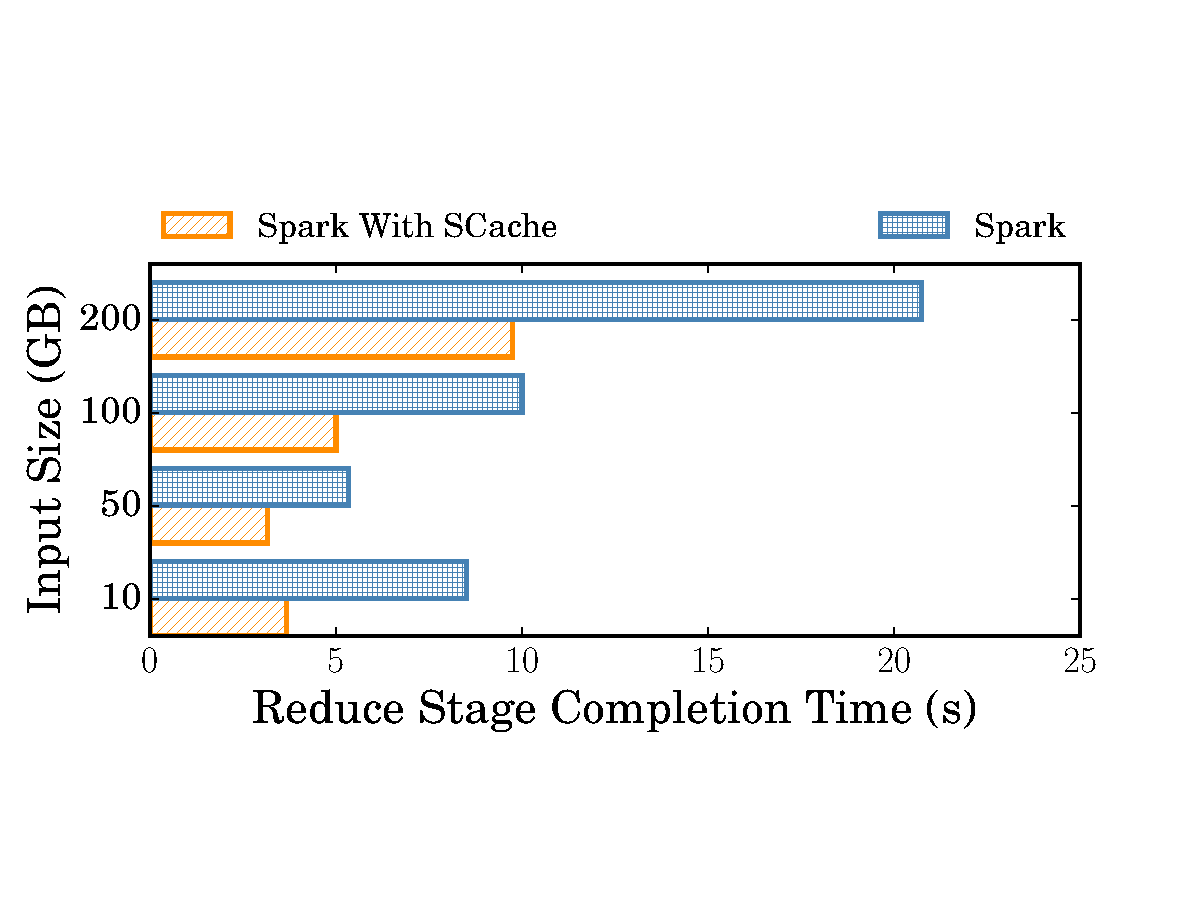
\includegraphics[width=\linewidth]{fig/tera}
				\caption{Reduce Stage of First Shuffle}
				\label{fig:terasort}
			\end{minipage}

			\begin{minipage}{\linewidth}
				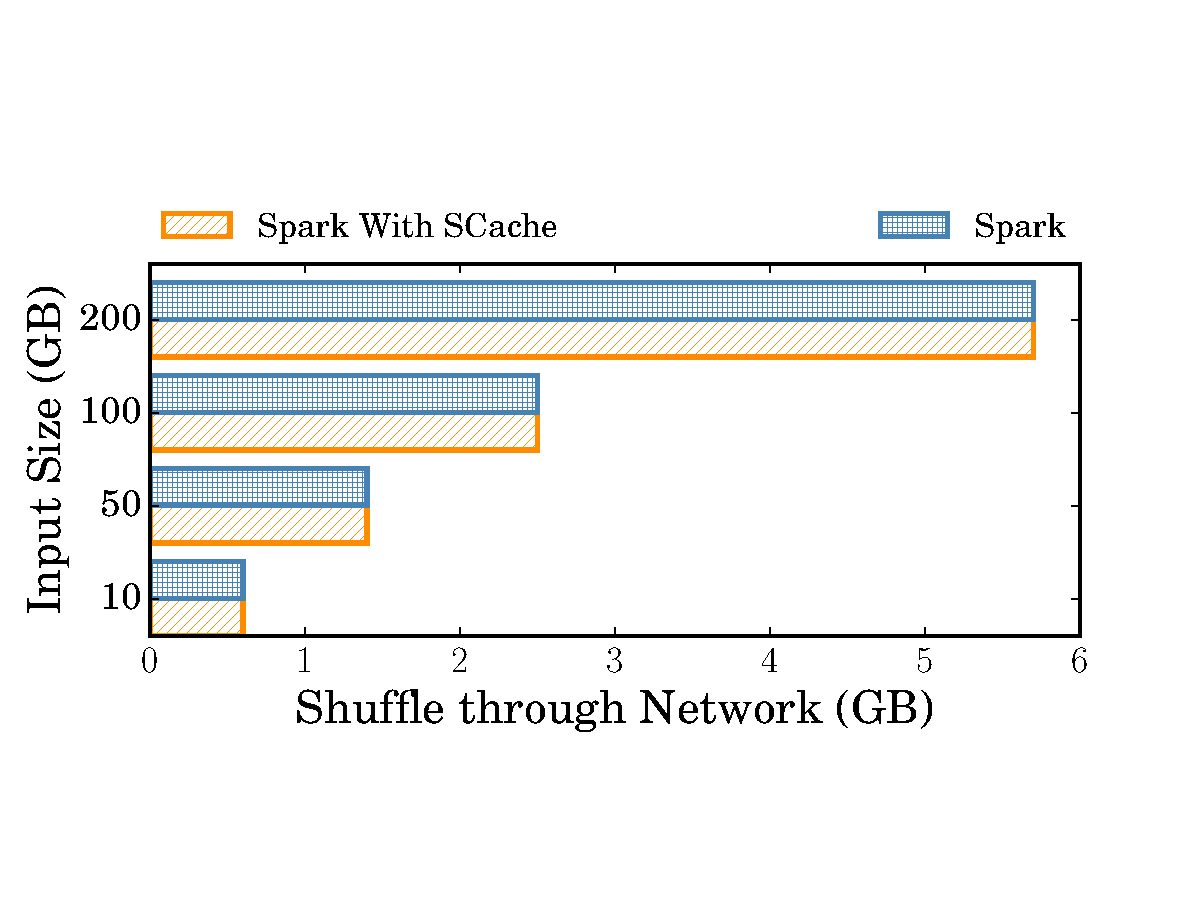
\includegraphics[width=\linewidth]{fig/tera_shuffle}
				\caption{Network Traffic of Second Shuffle}
				\label{fig:terashuffle}
			\end{minipage}
		\end{subfigure}
		\caption{Terasort Evaluation}
	\end{minipage}
\end{figure*}

\subsection{Setup}\label{stepup}
We modified Spark to enable shuffle optimization of SCache as a representative.
The shuffle configuration of Spark is set to the default\footnote{http://spark.apache.org/docs/1.6.2/configuration.html}. 
We run the experiments on a 50-node m4.xlarge cluster on Amazon EC2\footnote{http://aws.amazon.com/ec2/}. 
Each node has 16GB memory and 4 CPUs. The network bandwidth provided by Amazon is insufficient. 
Our evaluations reveal the bandwidth is only about 300 Mbps (see Figure \ref{fig:util}).

\subsection{Simple DAG Analysis}\label{simpledag}
%\subsubsection{Hardware Utilization}
We first run the same single shuffle test shown in Figure \ref{fig:util}. 
For each stage, we run 5 rounds of tasks with different input size. 
As shown in Figure \ref{fig:scache_util}, the hardware utilization is captured from one node during the job. 
Note that since the completion time of whole job is about $50\%$ less than Spark without SCache, the duration of Figure \ref{fig:scache_util} is cut in half as well. 
An overlap among CPU, disk, and network can be easily observed in Figure \ref{fig:scache_util}. 
It is because the decoupling of shuffle prevents the computing resource from being blocked by I/O operations. 
On the one hand, the decoupling of shuffle write helps free the slot earlier, so that it can be re-scheduled to a new map task.
On the other hand, with the help of shuffle pre-fetching, the decoupling of shuffle read significantly decreases the CPU idle time at the beginning of a reduce task.
At the same time, SCache manages the hardware resources to store and transfer shuffle data without interrupting the computing process.
As a result, the utilization and multiplexing of hardware resource are increased, thus improving the performance of Spark. 
% \begin{figure}
% 	%\vspace*{-0.01cm}
% 	\begin{subfigure}{\linewidth}
% 		\centering
% 		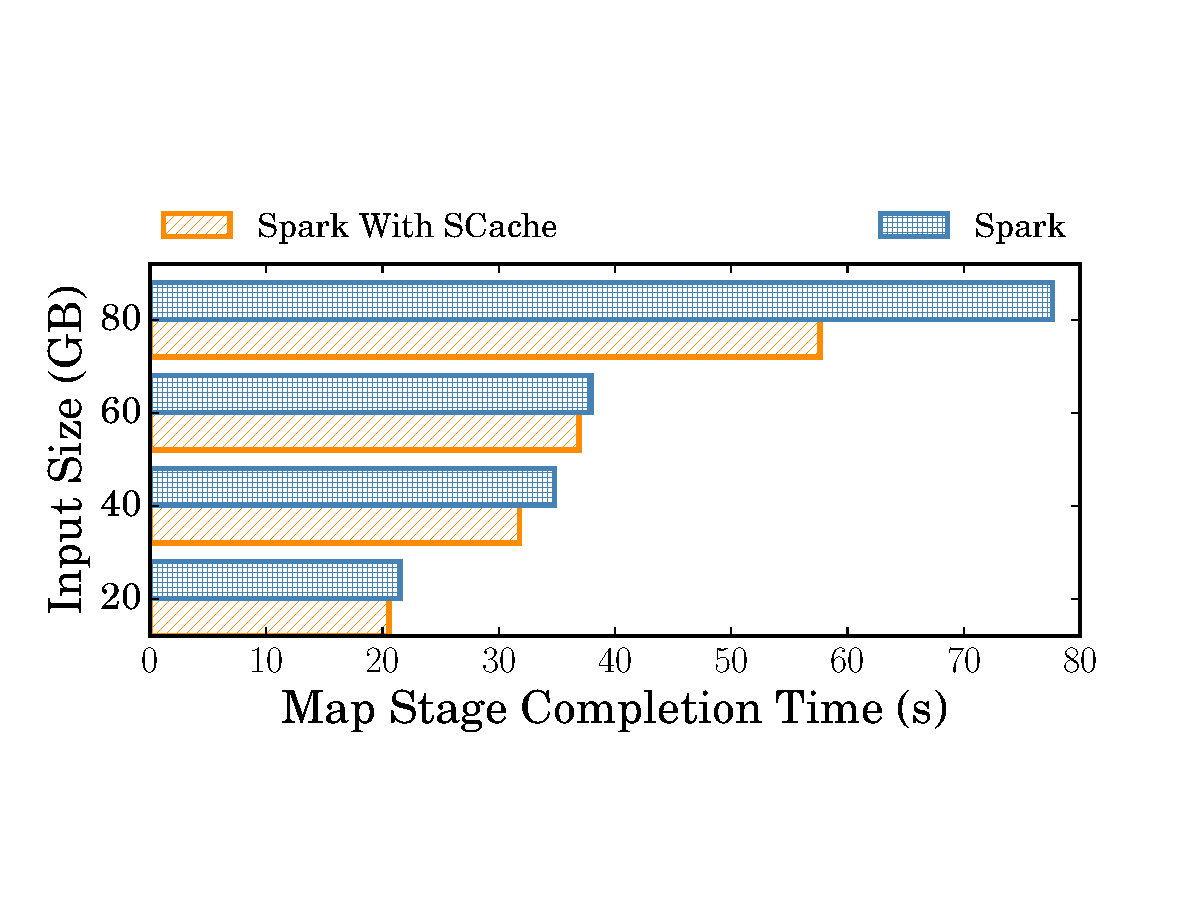
\includegraphics[width=0.6\linewidth]{fig/groupbymapstage}
% 		\caption{Map Stage Completion Time Comparison}
% 		\label{fig:mapstage}
% 	\end{subfigure}
% 	\begin{subfigure}{\linewidth}
% 		\centering
% 		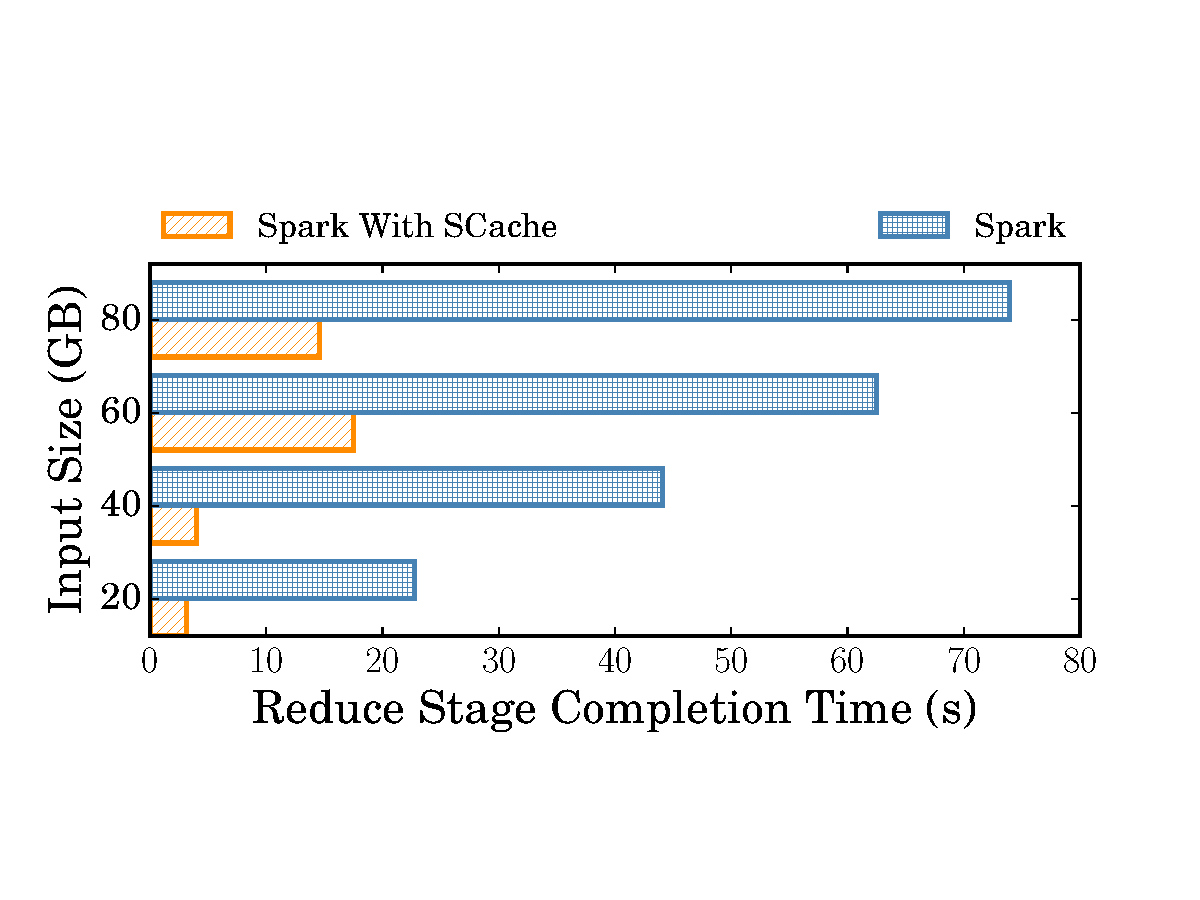
\includegraphics[width=0.6\linewidth]{fig/groupbyreducestage}
% 		\caption{Reduce Stage Completion Time Comparison}
% 		\label{fig:reducestage}
% 	\end{subfigure}
% 	\caption{Stage Completion Time of Single Shuffle Test}
% 	\label{fig:singleshuffle}
% \end{figure}

% \begin{figure}
% 	\begin{subfigure}{\linewidth}
% 		\centering
% 		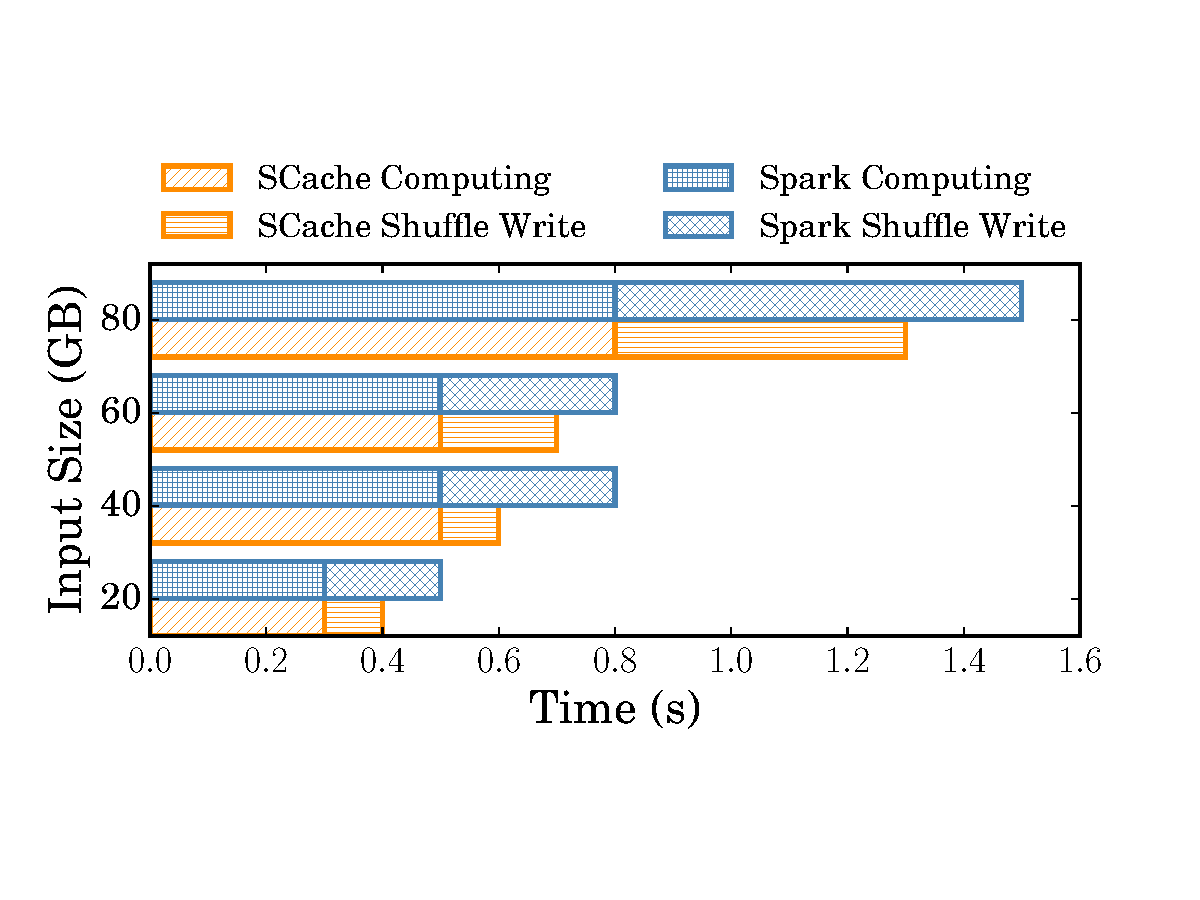
\includegraphics[width=0.6\linewidth]{fig/groupbymaptask}
% 		\caption{Median Task Details in Map Stages}
% 		\label{fig:maptask}
% 	\end{subfigure}
% 	\begin{subfigure}{\linewidth}
% 		\centering
% 		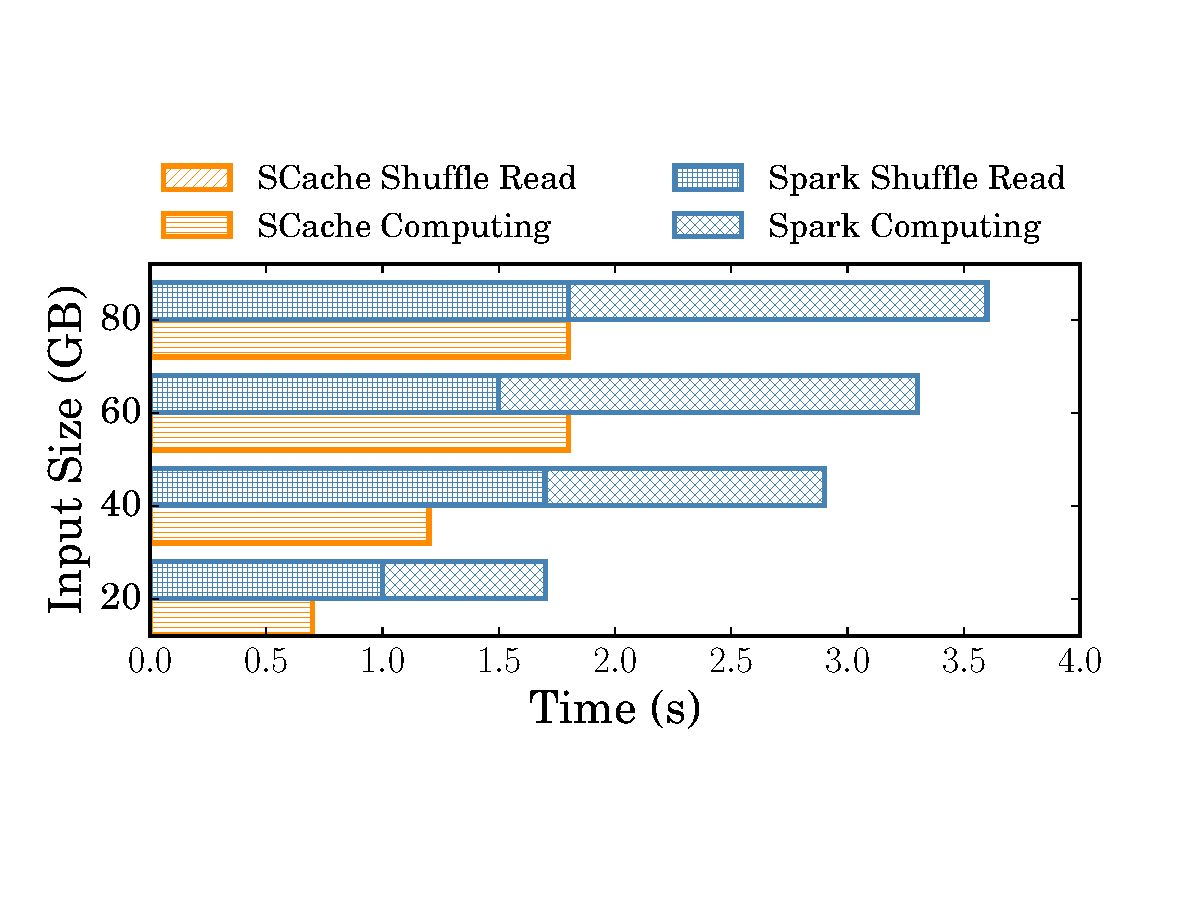
\includegraphics[width=0.6\linewidth]{fig/groupbyreducetask}
% 		\caption{Median Task Details in Reduce Stages}
% 		\label{fig:reducetask}
% 	\end{subfigure}
% 	\caption{Median Task Completion Time of Single Shuffle Test}
% 	\label{fig:singleshuffletask}
% \end{figure}
The performance evaluation in Figure \ref{fig:singleshuffletask} shows the consistent results with our observation of hardware utilization. 
% By running Spark with SCache, the completion time of map stage can be reduced $10\%$ on average. 
% For reduce stage, instead, SCache achieves a ~$75\%$ performance gain in the completion time of the reduce stage.
% A detail analysis into the nutshell of varied overall performance gain on different stages is presented with Figure \ref{fig:singleshuffletask}. 
For each stage, we pick the task that has median completion time. 
In the map task, the disk operations are replaced by the memory copies to decouple the shuffle write. 
It helps eliminate ~40\% of shuffle write time (Figure \ref{fig:maptask}), which leads to a $10\%$ improvement of map stage completion time in Figure \ref{fig:mapstage}. 
Note that the shuffle write time can be observed even with the optimization of SCache. 
The reason is that before moving data out of Spark's JVM, the serialization is inevitable and CPU intensive \cite{makingsense}. 

In the reduce task, most of the shuffle overhead is introduced by network transfer delay. 
By doing shuffle data pre-fetching based on the pre-scheduling results, the explicit network transfer is perfectly overlapped in the map stage. 
With the help of the co-scheduling scheme, SCache guarantees that each reduce task has the benefit of shuffle pre-fetching. 
The in-memory cache of shuffle data further reduce the shuffle read time. 
As a result, the combination of these optimizations decreases ~$100\%$ overhead of the shuffle read in a reduce task (Figure \ref{fig:reducetask}). 
In addition, the heuristic algorithm can achieve a balanced pre-scheduling result, thus providing ~$80\%$ improvement in reduce stage completion time (Figure \ref{fig:reducestage}).

In overall, SCache can help Spark decrease by ~$89\%$ overhead of the whole shuffle process. 

\subsection{Terasort}
We also evaluate Terasort\footnote{https://github.com/ehiggs/spark-terasort}-a recognized shuffle intensive benchmark for distributed system analysis.
Terasort consists of two consecutive shuffles. 
The first shuffle reads the input data and uses a hash partition function for re-partitioning. 
As shown in Figure \ref{fig:terasort}, Spark with SCache runs 2 $\times$ faster during the reduce stage of the first shuffle, which is consistent with the results in Section \ref{simpledag}. 
It further proves the effectiveness of SCache's optimization.

The second shuffle of Terasort partitions the data through a Spark RangePartitioner. 
% As the range bounds set by range partitioner almost match the same pattern of the first shuffle, almost $93\%$ of input data is from one particular map task for each reduce task. So we take the second shuffle as an extreme case to evaluate the scheduling locality for SCache.
In the second shuffle, almost $93\%$ of input data of a reduce task is produced by one particular map task. 
So we take the second shuffle as an extreme case to evaluate the heuristic locality swap of SCache.
In this shuffle, Spark schedules a reduce task to the node that produces most input data. 
By doing this, Spark minimizes the shuffle data through network. 
At the same time, Figure \ref{fig:terashuffle} reveals that SCache produces exactly same network traffic as Spark. 
It implies that the heuristic locality swap of SCache can obtain the best locality while balancing the load. 

\begin{figure*}
	\centering
	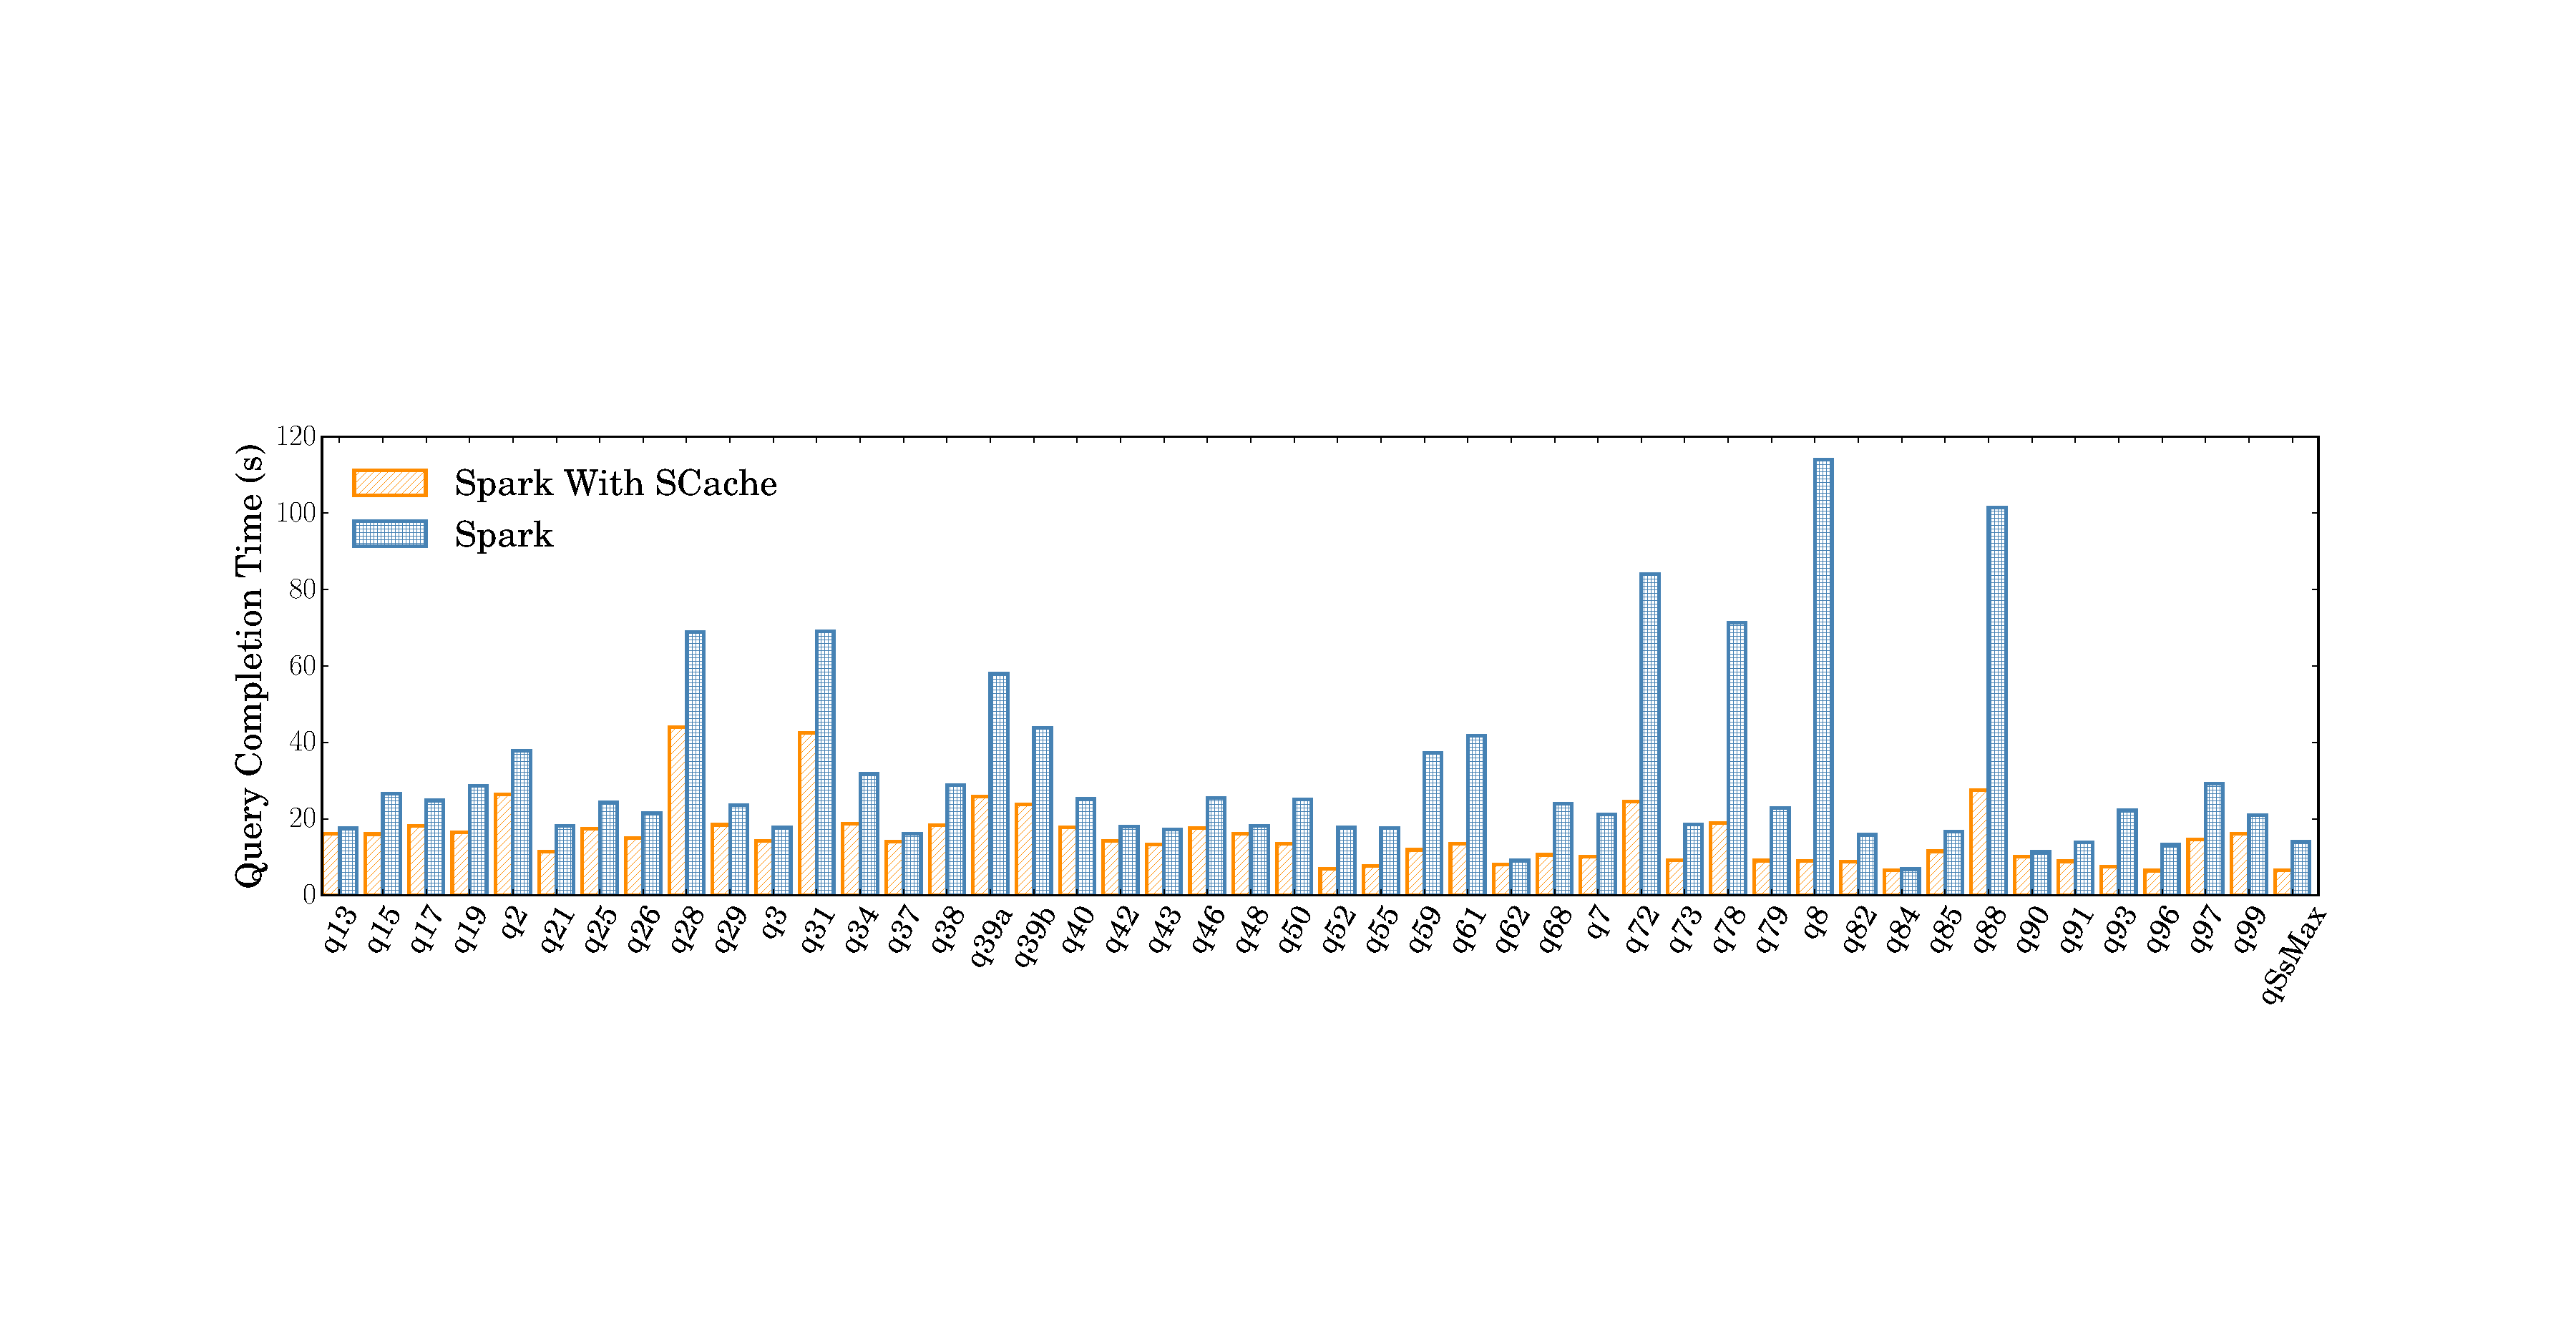
\includegraphics[width=0.85\textwidth]{fig/tpcds}
	\caption{TPC-DS Benchmark Evaluation}
	\label{fig:tpcds}
	\vspace{-1em}
\end{figure*}
\begin{figure}
	\centering
	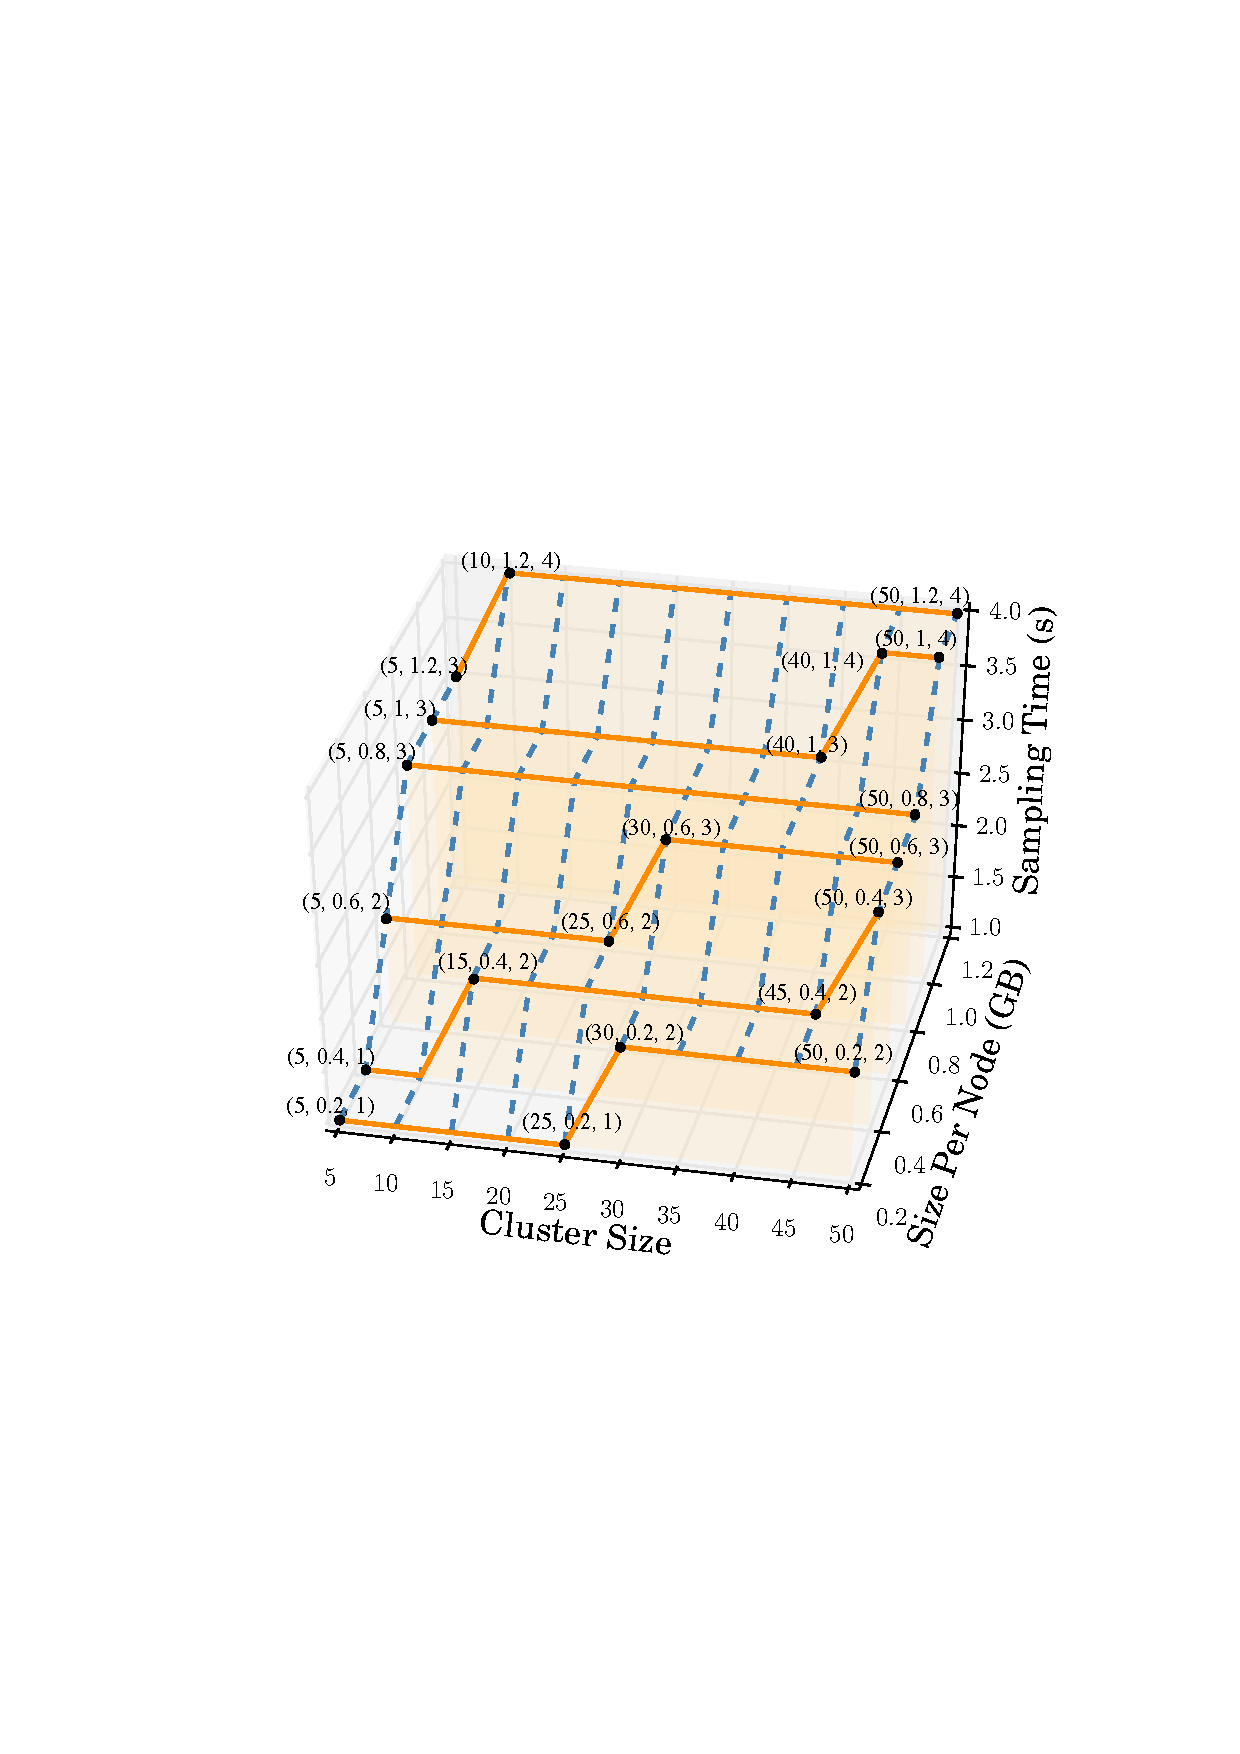
\includegraphics[width=0.6\linewidth]{fig/sampling}
	\caption{Sampling Overhead}
	\label{fig:sampling}
	\vspace{-1em}
\end{figure}

{\color{blue}
\subsection{Hadoop MapReduce with SCache}

To prove SCache compatibility as a cross-framework plug-in, we also implemented SCache on Hadoop MapReduce as the external shuffle service and co-scheduler. Although \textit{pre-scheduling reduce tasks} is not critical for the simple DAG computing in Hadoop MapReduce, some shuffle-heavy jobs on Hadoop Madpreduce can still be optimized by SCache shuffle data management.

Figure \ref{fig:hadoop_terasort} shows the hardware resource utilization of Hadoop MapReduce running Terasort. Both figures have the same proportion of time. Hadoop MapReduce with SCache brings 15\% of total time optimization with 384GB input data size. 
As shown in the Figure \ref{fig:hadoop_terasort_origin}, Hadoop MapReduce without SCache writes intermediate data locally in the map phase. The shuffle phase and reduce phase start simultaneously. Because the large amount of shuffle data reaches the network bottleneck, the beginning part of reduce needs to wait needs to wait for network transfer. This causes the CPU resources to be idle. 
As shown in the Figure \ref{fig:hadoop_terasort_scache}, Hadoop Madpreduce with SCache start pre-fetching in the map phase. This avoids the reduce phase waiting for the shuffle data. Furthermore, pre-fetching utilizes the idle IO throughput in the map phase. As shown in Figure \ref{fig:hadoop_terasort_time}, after better fine-grained utilization of hardware resources, Hadoop MapReduce with SCache optimize Terasort overall completion time by up to 15\% and an average of 13\% with input data sizes from 128GB to 512GB.
}

\begin{figure}
	\centering
	\begin{minipage}[hb]{\linewidth}
		\begin{subfigure}{\linewidth}
			\begin{minipage}{\linewidth}
				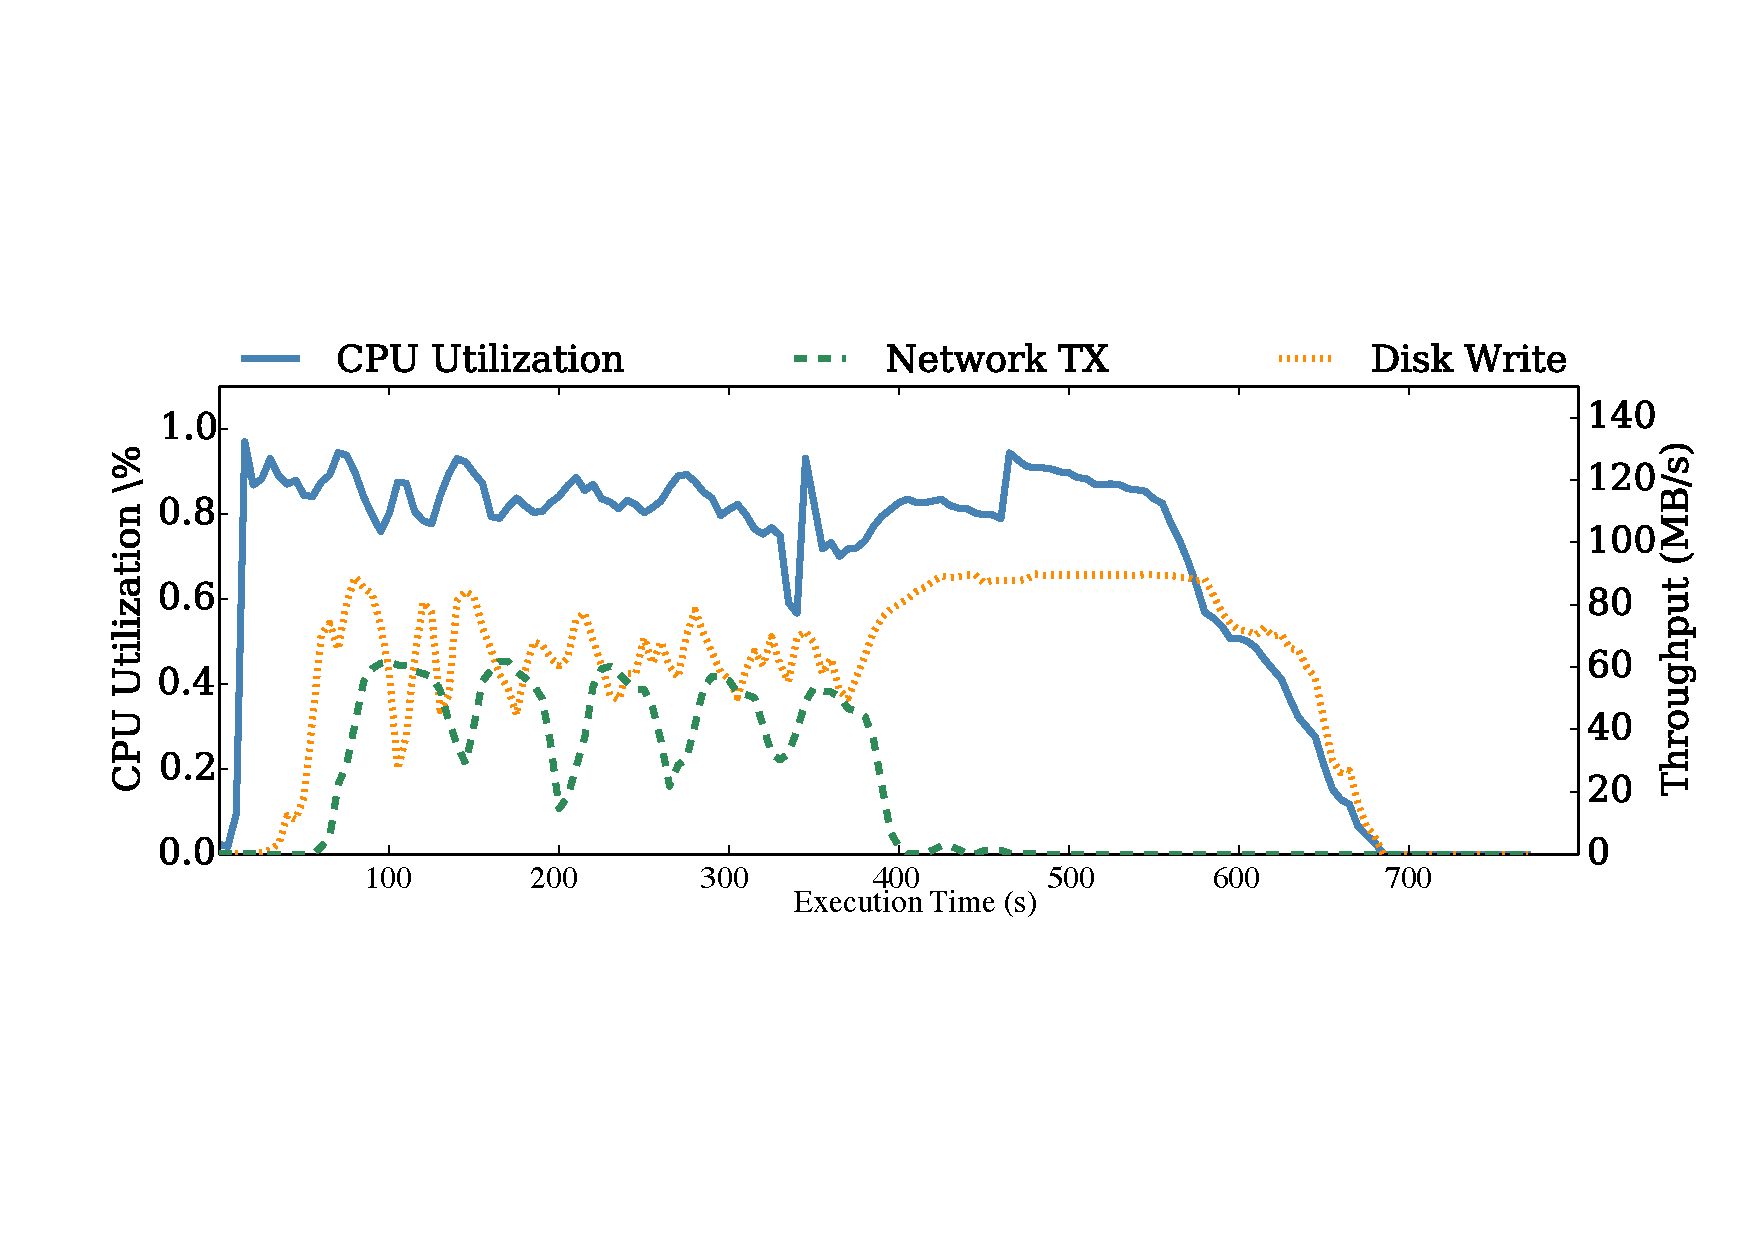
\includegraphics[width=\linewidth]{fig/hadoop_terasort_scache}
				\caption{\color{blue}Hadoop MapReduce With SCache}
				\label{fig:hadoop_terasort_scache}
			\end{minipage}
			\begin{minipage}{\linewidth}
				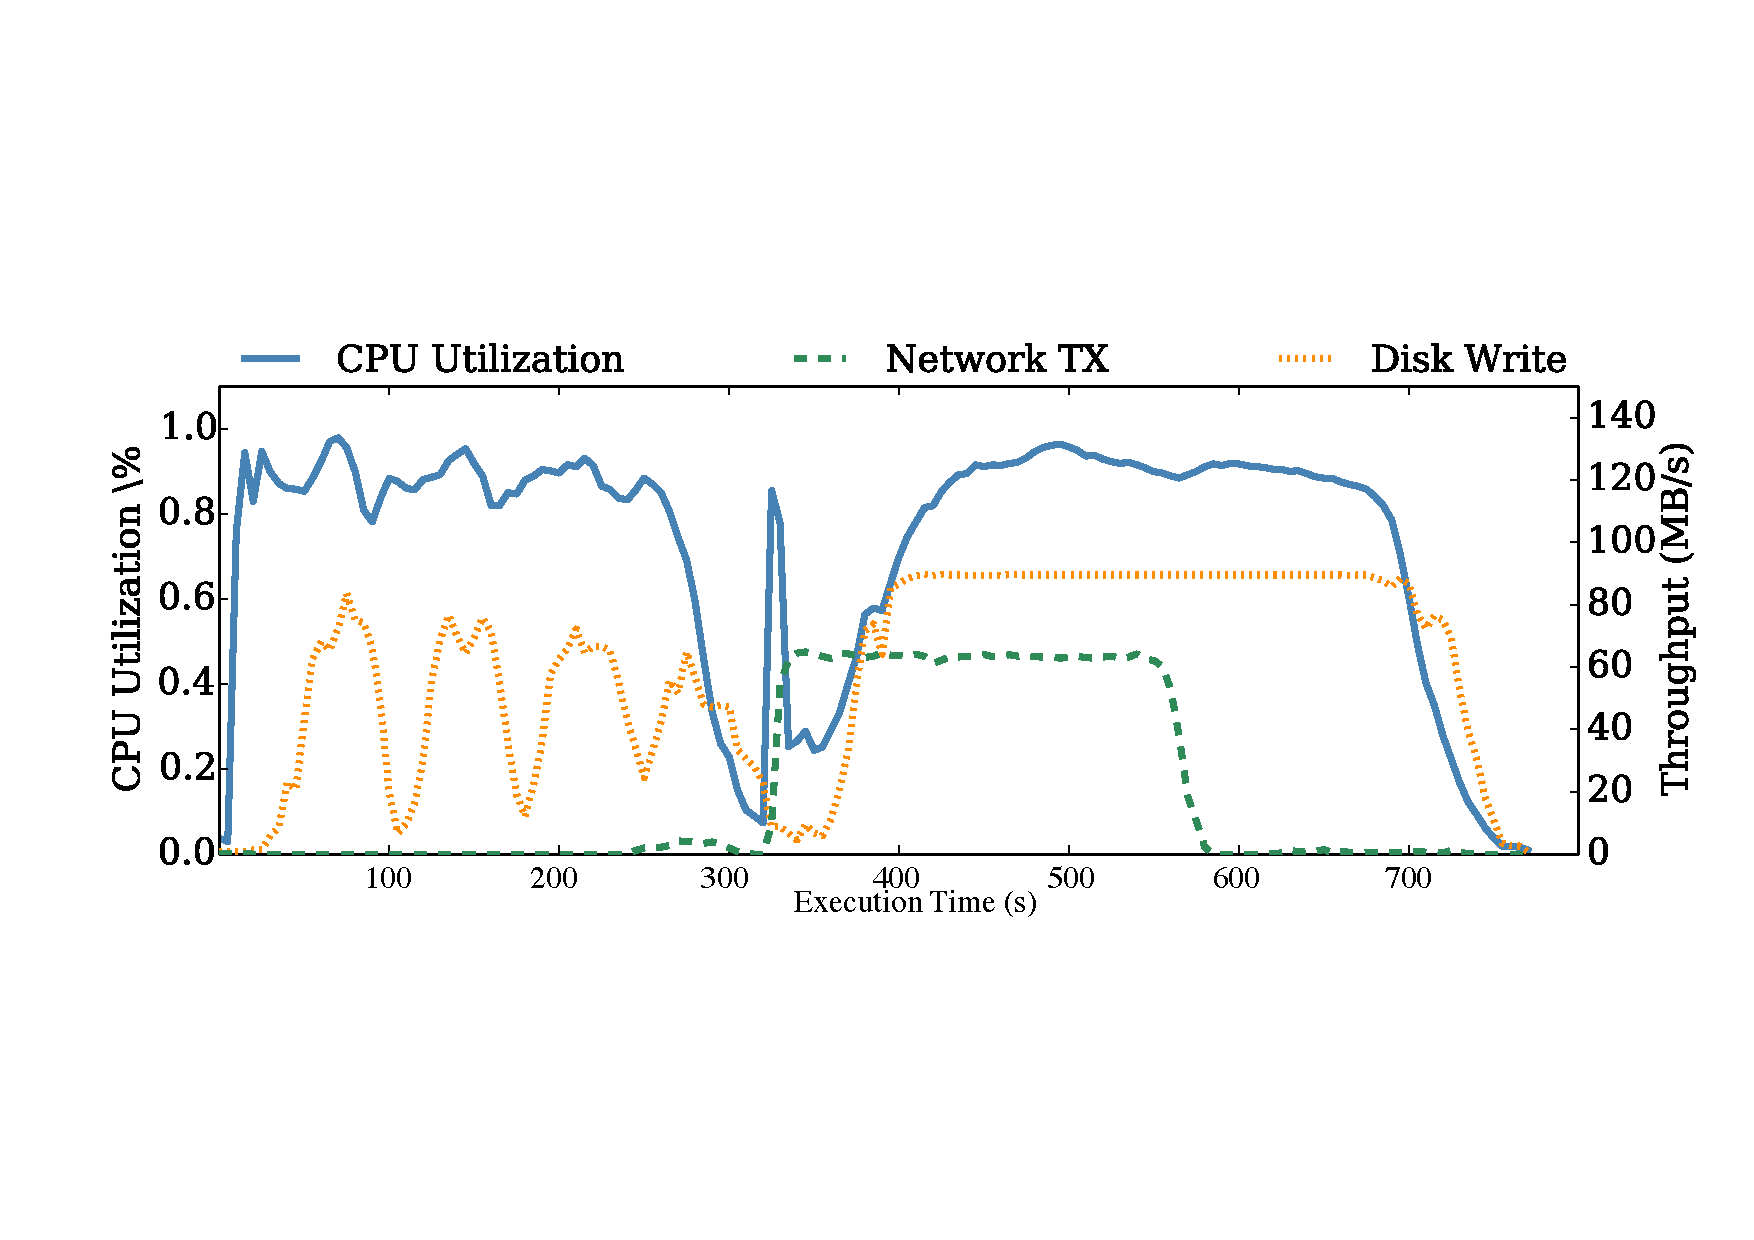
\includegraphics[width=\linewidth]{fig/hadoop_terasort_origin}
				\caption{\color{blue}Hadoop MapReduce Without SCache}
				\label{fig:hadoop_terasort_origin}
			\end{minipage}
		\end{subfigure}
		\caption{\color{blue}CPU utilization and I/O throughput of a node during a Hadoop MapReduce Terasort job}
		\label{fig:hadoop_terasort}
	\end{minipage}
\end{figure}

\begin{figure}
	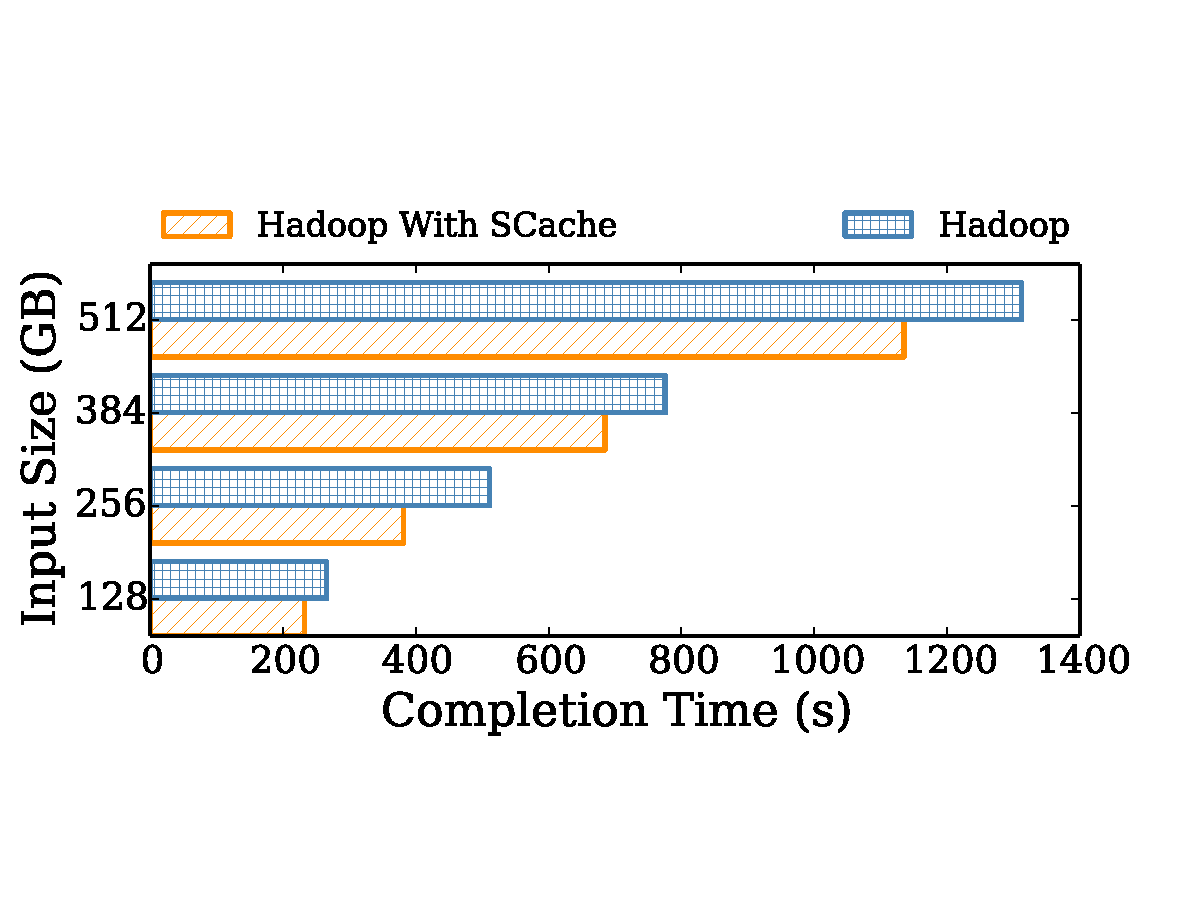
\includegraphics[width=\linewidth]{fig/hadoop_terasort_time}
	\caption{\color{blue}Hadoop MapReduce Terasort completion time}
	\label{fig:hadoop_terasort_time}
\end{figure}

\subsection{Production Workload}
We also evaluate some queries from TPC-DS\footnote{http://www.tpc.org/tpcds/}. 
TPC-DS benchmark is designed for modeling multiple users submitting varied queries (e.g. ad-hoc, interactive OLAP, data mining, etc.). 
TPC-DS contains 99 queries and is considered as the standardized industry benchmark for testing big data systems. 
% We evaluate the performance of Spark with SCache by picking some of the TPC-DS queries with shuffle intensive attribute. 
As shown in Figure \ref{fig:tpcds}, the horizontal axis is query name and the vertical axis is query completion time. 
Note that we skip some queries due to the compatible issues. 
Spark with SCache outperforms the original Spark in almost all tested queries. 
Furthermore, in many queries, Spark with SCache outperforms original Spark by an order of magnitude. 
It is because that those queries contain shuffle-heavy operations such as "groupby", "union", etc.
The overall reduction portion of query time that SCache achieved is 40\% on average. 
Since this evaluation presents the overall job completion time of queries, we believe that our shuffle optimization is promising.
% \begin{figure}
% 	\begin{subfigure}{\linewidth}
% 		\centering
% 		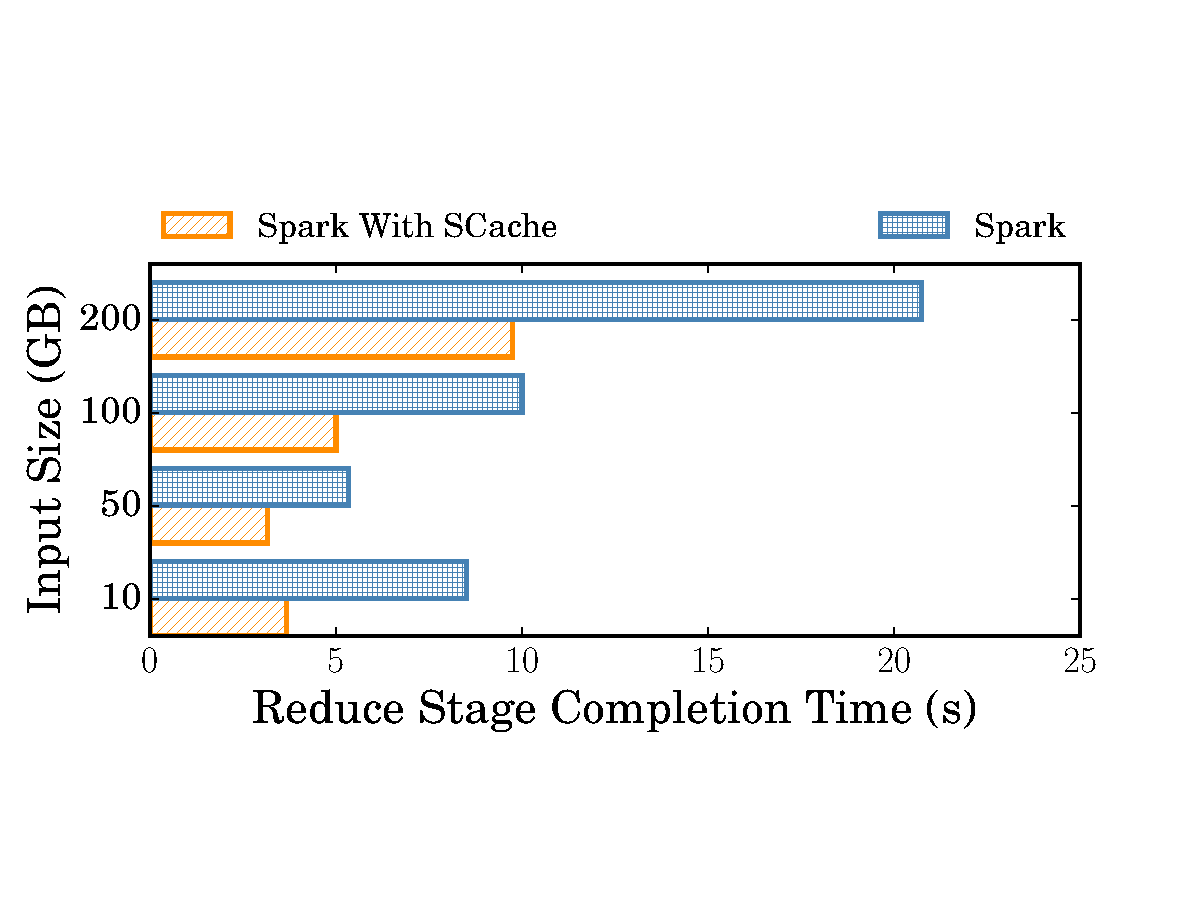
\includegraphics[width=0.6\linewidth]{fig/tera}
% 		\caption{Reduce Stage Completion Time Comparison of First Shuffle}
% 		\label{fig:terasort}
% 	\end{subfigure}
% 	\vspace{0.08cm}
% 	\begin{subfigure}{\linewidth}
% 		\centering
% 		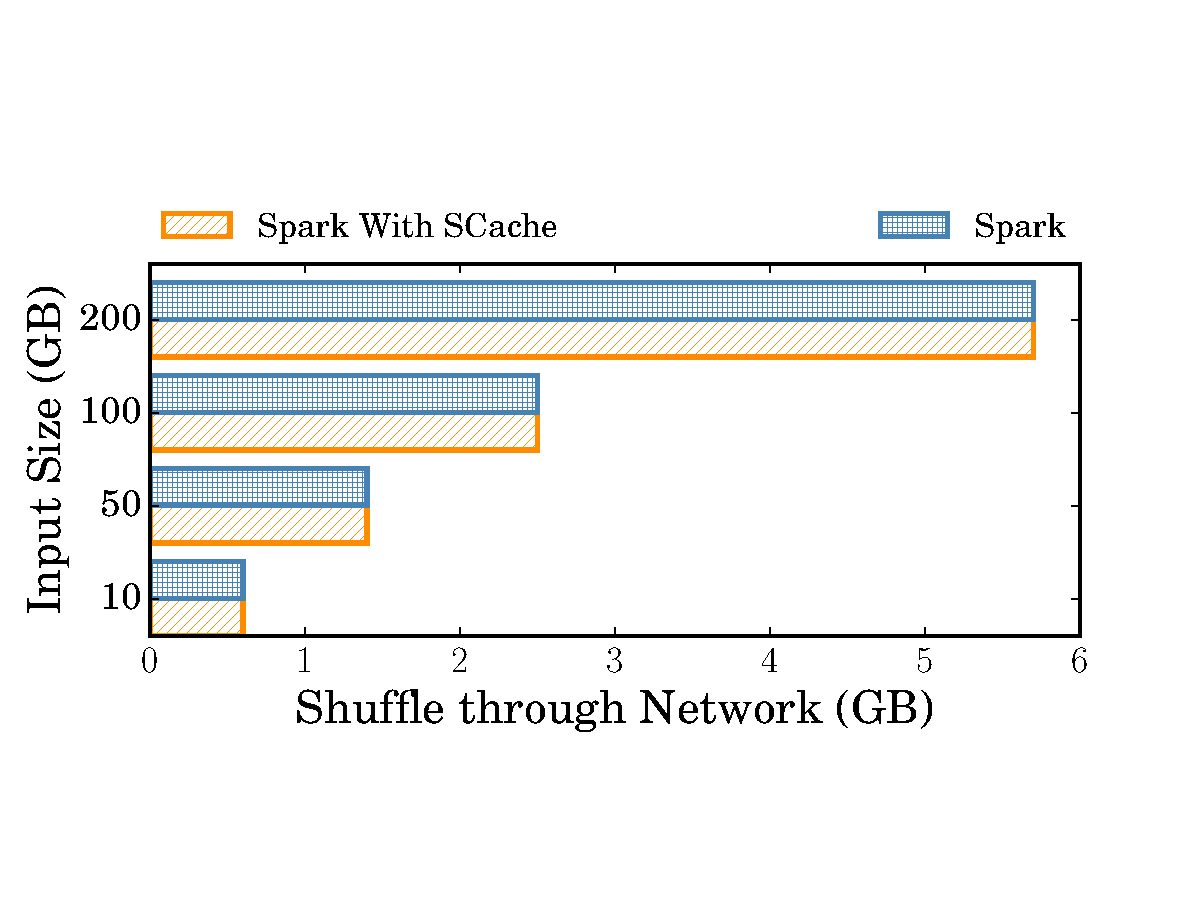
\includegraphics[width=0.6\linewidth]{fig/tera_shuffle}
% 		\caption{Shuffle Data through Network Comparison of Second Shuffle}
% 		\label{fig:terashuffle}
% 	\end{subfigure}
% 	\caption{Terasort Evaluation}
% \end{figure}
\subsection{Overhead of Sampling}
We evaluate the overhead of sampling with different input sizes and numbers of nodes. 
In Figure \ref{fig:sampling}, the overhead of sampling only grows with the increase of input size on each node, but remains relatively stable when the cluster size scales up.
Since the shuffle data is short-lived, write-once, and read-once, the central controller of SCache does not have to collect and manage complex metadata. 
Meanwhile, most of the optimizations such as fetching and storing shuffle data are finished by workers independently. 
So the cost of pre-scheduling algorithm and memory management are unlikely to make the master become the bottleneck of the scalability.
Combined with the sampling overhead evaluation, we believe that SCache is scalable.

\section{Related Work}

{\color{black}
\textbf{Modeling}: Most representative DAG computing frameworks use similar \textit{Bulk Synchronize Parallel} (BSP)\cite{valiant1990bridging} model to control data synchronization in each computing phase, i.e. \textit{stage} in Spark, \textit{superstep} in Pregel\cite{malewicz2010pregel} and so on (Hadoop MapReduce can also be considered as a special case of only one superstep in BSP model). 
In the process of optimizing the shuffle phases between adjacent computing phases, we design a performance model to assist in analyzing computing process.
There are also lots of performance models for MapReduce have been proposed, such as \cite{verma2011aria, khan2016hadoop, herodotou2011hadoop, chen2014cresp}.
Verma et al. \cite{verma2011aria} proposed the ARIA model to estimate the required resources based on the job information, the amount of input data and a specified soft deadline.
Khan et al. \cite{khan2016hadoop} proposed the HP model which extends the ARIA model. The HP model adds scaling factors and uses a simple linear regression to estimate the job execution time on larger datasets.
In \cite{herodotou2011hadoop}, Herodotou proposed a detailed set of mathematical performance models for describing the execution of a MapReduce job. The execution is separated into the phases: Read, Map, Collect, Spill, Merge, Shuffle, Merge, and Reduce. The set of performance models describe each above-mentioned phases and combine into an overall MapReduce job model. 
Chen et al. \cite{chen2014cresp} proposed the CRESP model which is a cost model that estimates the performance of a job then 
provisions the resources for the job.

However, the above models are not able to accurately describe the overhead caused by the shuffle process under different scheduling strategies. 
Different from these models, our FRQ model quantifies computing and I/O resources and displays them in the time dimension. FRQ model focuses on describing the overhead caused by the shuffle process in different scheduling strategies, which satisfy our demand.
}

\textbf{Pre-scheduling}: Slow-start from Apache Hadoop MapReduce is a classic approach to handle shuffle overhead. 
Starfish \cite{starfish} gets sampled data statics for self-tuning system parameters (e.g. slow-start, etc). 
DynMR \cite{dynmr} dynamically starts reduce tasks in late map stage. 
All of them have the explicit I/O time in occupied slots. 
SCache instead starts shuffle pre-fetching without consuming slots. 
iShuffle \cite{guo2017ishuffle} decouples shuffle from reducers and designs a centralized shuffle controller. 
But it can neither handle multiple shuffles nor schedule multiple rounds of reduce tasks. 
iHadoop \cite{ihadoop} aggressively pre-schedules tasks in multiple successive stages to start fetching shuffle. 
But we have proved that randomly assign tasks may hurt the overall performance in Section \ref{randomassign}. 
Different from these works, SCache pre-schedules multiple shuffles without breaking load balancing. 

%  by combining DAG information and heuristic algorithms.
\textbf{Delay-scheduling}: Delay Scheduling \cite{delay} delays tasks assignment to get better data locality, which can reduce the network traffic. 
ShuffleWatcher \cite{shufflewatcher} delays shuffle fetching when the network is saturated. 
At the same time, it achieves better data locality. 
Both Quincy \cite{quincy} and Fair Scheduling \cite{preemptive} can reduce shuffle data by optimizing data locality of map tasks. 
But all of them cannot mitigate explicit I/O in both map and reduce tasks. 
In addition, their optimizations fluctuate under different network performances and data distributions, whereas SCache can provide a stable performance gain by shuffle data pre-fetching and in-memory caching.

\textbf{Network layer optimization}: Varys \cite{varys} and Aalo \cite{aalo} provide the network layer optimization for shuffle transfer. 
Though the efforts are limited throughout whole shuffle process, they can be easily applied on SCache to further improve the performance.
\section{Conclusion}
In this paper, we present SCache, a cross-framework shuffle optimization for DAG computing frameworks. 
SCache decouples the shuffle from computing tasks and leverages memory to store shuffle data. 
By tasks pre-scheduling and shuffle data pre-fetching with application context, SCache significantly mitigates the shuffle overhead. 
%  {\color{red}
%  Our implementation with Spark and evaluations show that SCache can provide a promising speedup to the DAG framework. 
%  }
{\color{blue}
Our evaluations on Spark and Hadoop Mapreduce with SCache show that SCache can provide a promising speedup. 
Furthermore, we propose \textit{Framework Resources Quantification}(FRQ) model to assist in analyzing shuffle process of DAG computing frameworks. At last we use FRQ model to verify SCache shuffle optimization by mathematics.
Therefore, with the shared defects of shuffle among different frameworks, we believe that the optimization of SCache is general and easy to adapt. 
}

\section{Acknowledge}
This work was supported in part by National Key Research \& Development Program of China (No. 2016YFB1000502), National NSF of China (NO. 61672344, 61525204, 61732010), and Shanghai Key Laboratory of Scalable Computing and Systems.

% The very first letter is a 2 line initial drop letter followed
% by the rest of the first word in caps (small caps for compsoc).
% 
% form to use if the first word consists of a single letter:
% \IEEEPARstart{A}{demo} file is ....
% 
% form to use if you need the single drop letter followed by
% normal text (unknown if ever used by the IEEE):
% \IEEEPARstart{A}{}demo file is ....
% 
% Some journals put the first two words in caps:
% \IEEEPARstart{T}{his demo} file is ....
% 
% Here we have the typical use of a "T" for an initial drop letter
% and "HIS" in caps to complete the first word.
% \IEEEPARstart{T}{his} demo file is intended to serve as a ``starter file''
% for IEEE Computer Society journal papers produced under \LaTeX\ using
% IEEEtran.cls version 1.8b and later.
% You must have at least 2 lines in the paragraph with the drop letter
% (should never be an issue)
% I wish you the best of success.

% \hfill mds
 
% \hfill August 26, 2015

% \subsection{Subsection Heading Here}
% Subsection text here.

% needed in second column of first page if using \IEEEpubid
%\IEEEpubidadjcol

% \subsubsection{Subsubsection Heading Here}
% Subsubsection text here.


% An example of a floating figure using the graphicx package.
% Note that \label must occur AFTER (or within) \caption.
% For figures, \caption should occur after the \includegraphics.
% Note that IEEEtran v1.7 and later has special internal code that
% is designed to preserve the operation of \label within \caption
% even when the captionsoff option is in effect. However, because
% of issues like this, it may be the safest practice to put all your
% \label just after \caption rather than within \caption{}.
%
% Reminder: the "draftcls" or "draftclsnofoot", not "draft", class
% option should be used if it is desired that the figures are to be
% displayed while in draft mode.
%
%\begin{figure}[!t]
%\centering
%\includegraphics[width=2.5in]{myfigure}
% where an .eps filename suffix will be assumed under latex, 
% and a .pdf suffix will be assumed for pdflatex; or what has been declared
% via \DeclareGraphicsExtensions.
%\caption{Simulation results for the network.}
%\label{fig_sim}
%\end{figure}

% Note that the IEEE typically puts floats only at the top, even when this
% results in a large percentage of a column being occupied by floats.
% However, the Computer Society has been known to put floats at the bottom.


% An example of a double column floating figure using two subfigures.
% (The subfig.sty package must be loaded for this to work.)
% The subfigure \label commands are set within each subfloat command,
% and the \label for the overall figure must come after \caption.
% \hfil is used as a separator to get equal spacing.
% Watch out that the combined width of all the subfigures on a 
% line do not exceed the text width or a line break will occur.
%
%\begin{figure*}[!t]
%\centering
%\subfloat[Case I]{\includegraphics[width=2.5in]{box}%
%\label{fig_first_case}}
%\hfil
%\subfloat[Case II]{\includegraphics[width=2.5in]{box}%
%\label{fig_second_case}}
%\caption{Simulation results for the network.}
%\label{fig_sim}
%\end{figure*}
%
% Note that often IEEE papers with subfigures do not employ subfigure
% captions (using the optional argument to \subfloat[]), but instead will
% reference/describe all of them (a), (b), etc., within the main caption.
% Be aware that for subfig.sty to generate the (a), (b), etc., subfigure
% labels, the optional argument to \subfloat must be present. If a
% subcaption is not desired, just leave its contents blank,
% e.g., \subfloat[].


% An example of a floating table. Note that, for IEEE style tables, the
% \caption command should come BEFORE the table and, given that table
% captions serve much like titles, are usually capitalized except for words
% such as a, an, and, as, at, but, by, for, in, nor, of, on, or, the, to
% and up, which are usually not capitalized unless they are the first or
% last word of the caption. Table text will default to \footnotesize as
% the IEEE normally uses this smaller font for tables.
% The \label must come after \caption as always.
%
%\begin{table}[!t]
%% increase table row spacing, adjust to taste
%\renewcommand{\arraystretch}{1.3}
% if using array.sty, it might be a good idea to tweak the value of
% \extrarowheight as needed to properly center the text within the cells
%\caption{An Example of a Table}
%\label{table_example}
%\centering
%% Some packages, such as MDW tools, offer better commands for making tables
%% than the plain LaTeX2e tabular which is used here.
%\begin{tabular}{|c||c|}
%\hline
%One & Two\\
%\hline
%Three & Four\\
%\hline
%\end{tabular}
%\end{table}


% Note that the IEEE does not put floats in the very first column
% - or typically anywhere on the first page for that matter. Also,
% in-text middle ("here") positioning is typically not used, but it
% is allowed and encouraged for Computer Society conferences (but
% not Computer Society journals). Most IEEE journals/conferences use
% top floats exclusively. 
% Note that, LaTeX2e, unlike IEEE journals/conferences, places
% footnotes above bottom floats. This can be corrected via the
% \fnbelowfloat command of the stfloats package.




% \section{Conclusion}
% The conclusion goes here.





% if have a single appendix:
%\appendix[Proof of the Zonklar Equations]
% or
%\appendix  % for no appendix heading
% do not use \section anymore after \appendix, only \section*
% is possibly needed

% use appendices with more than one appendix
% then use \section to start each appendix
% you must declare a \section before using any
% \subsection or using \label (\appendices by itself
% starts a section numbered zero.)
%


% \appendices
% \section{Proof of the First Zonklar Equation}
% Appendix one text goes here.

% you can choose not to have a title for an appendix
% if you want by leaving the argument blank
% \section{}
% Appendix two text goes here.


% use section* for acknowledgment
% \ifCLASSOPTIONcompsoc
%   % The Computer Society usually uses the plural form
%   \section*{Acknowledgments}
% \else
%   % regular IEEE prefers the singular form
%   \section*{Acknowledgment}
% \fi


% The authors would like to thank...


% % Can use something like this to put references on a page
% % by themselves when using endfloat and the captionsoff option.
% \ifCLASSOPTIONcaptionsoff
%   \newpage
% \fi



% trigger a \newpage just before the given reference
% number - used to balance the columns on the last page
% adjust value as needed - may need to be readjusted if
% the document is modified later
%\IEEEtriggeratref{8}
% The "triggered" command can be changed if desired:
%\IEEEtriggercmd{\enlargethispage{-5in}}

% references section

% can use a bibliography generated by BibTeX as a .bbl file
% BibTeX documentation can be easily obtained at:
% http://mirror.ctan.org/biblio/bibtex/contrib/doc/
% The IEEEtran BibTeX style support page is at:
% http://www.michaelshell.org/tex/ieeetran/bibtex/
\bibliographystyle{IEEEtran}
% argument is your BibTeX string definitions and bibliography database(s)
\bibliography{biblio}
%
% <OR> manually copy in the resultant .bbl file
% set second argument of \begin to the number of references
% (used to reserve space for the reference number labels box)
% \begin{thebibliography}{1}

% \bibitem{IEEEhowto:kopka}
% H.~Kopka and P.~W. Daly, \emph{A Guide to \LaTeX}, 3rd~ed.\hskip 1em plus
%   0.5em minus 0.4em\relax Harlow, England: Addison-Wesley, 1999.


% \end{thebibliography}
% biography section
% 
% If you have an EPS/PDF photo (graphicx package needed) extra braces are
% needed around the contents of the optional argument to biography to prevent
% the LaTeX parser from getting confused when it sees the complicated
% \includegraphics command within an optional argument. (You could create
% your own custom macro containing the \includegraphics command to make things
% simpler here.)
\begin{IEEEbiography}[{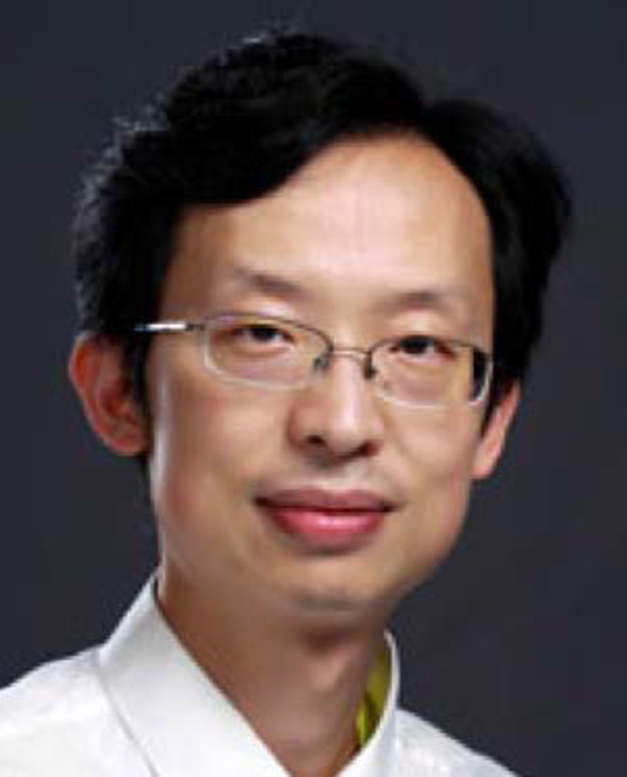
\includegraphics[width=1in,height=1.25in,clip,keepaspectratio]{./fig/author/Rui_Ren}}]{Rui Ren}
was born in Shaanxi, China, in 1978. He received the B.S. and M.S. degrees from Shanghai Jiao Tong University, China, in 2000 and 2004, respectively. He is currently a lecturer in the School of Software, Shanghai Jiao Tong University, China.
\end{IEEEbiography}

\begin{IEEEbiography}[{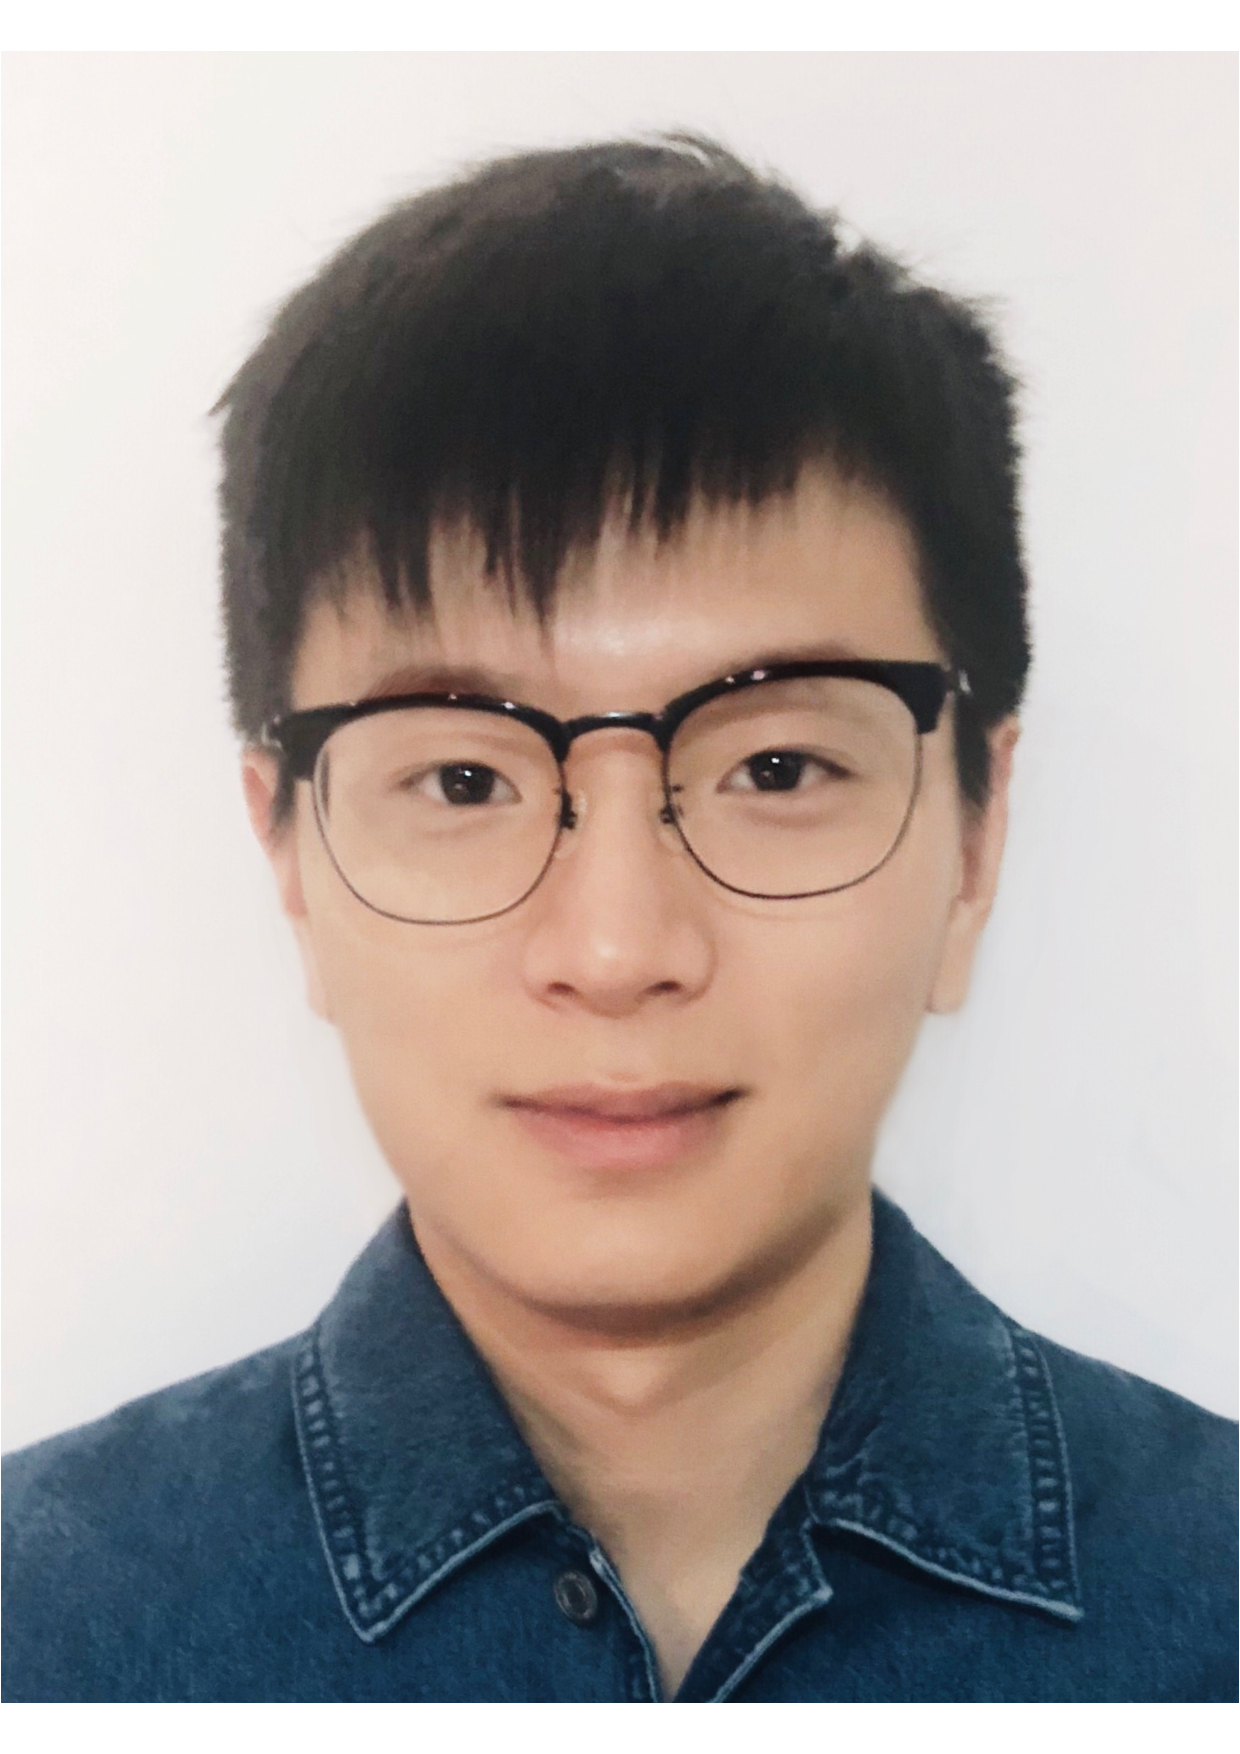
\includegraphics[width=1in,height=1.25in,clip,keepaspectratio]{./fig/author/Chunghsuan_Wu}}]{Chunghsuan Wu}
received the BE degree from Shanghai Jiao Tong University, China, in 2017. He is currently pursuing a ME degree in Shanghai Jiao Tong University, China. His research interests mainly focus on distributed computing.
\end{IEEEbiography}

\begin{IEEEbiography}[{\includegraphics[width=1in,height=1.25in,clip,keepaspectratio]{./fig/author/ZhouWang_Fu}}]{Zhouwang Fu}
is a graduated Master student of Shanghai Jiao Tong University in China. He received his Bachelor and Master degree in software engineering Shanghai Jiao Tong University.
\end{IEEEbiography}

\begin{IEEEbiography}[{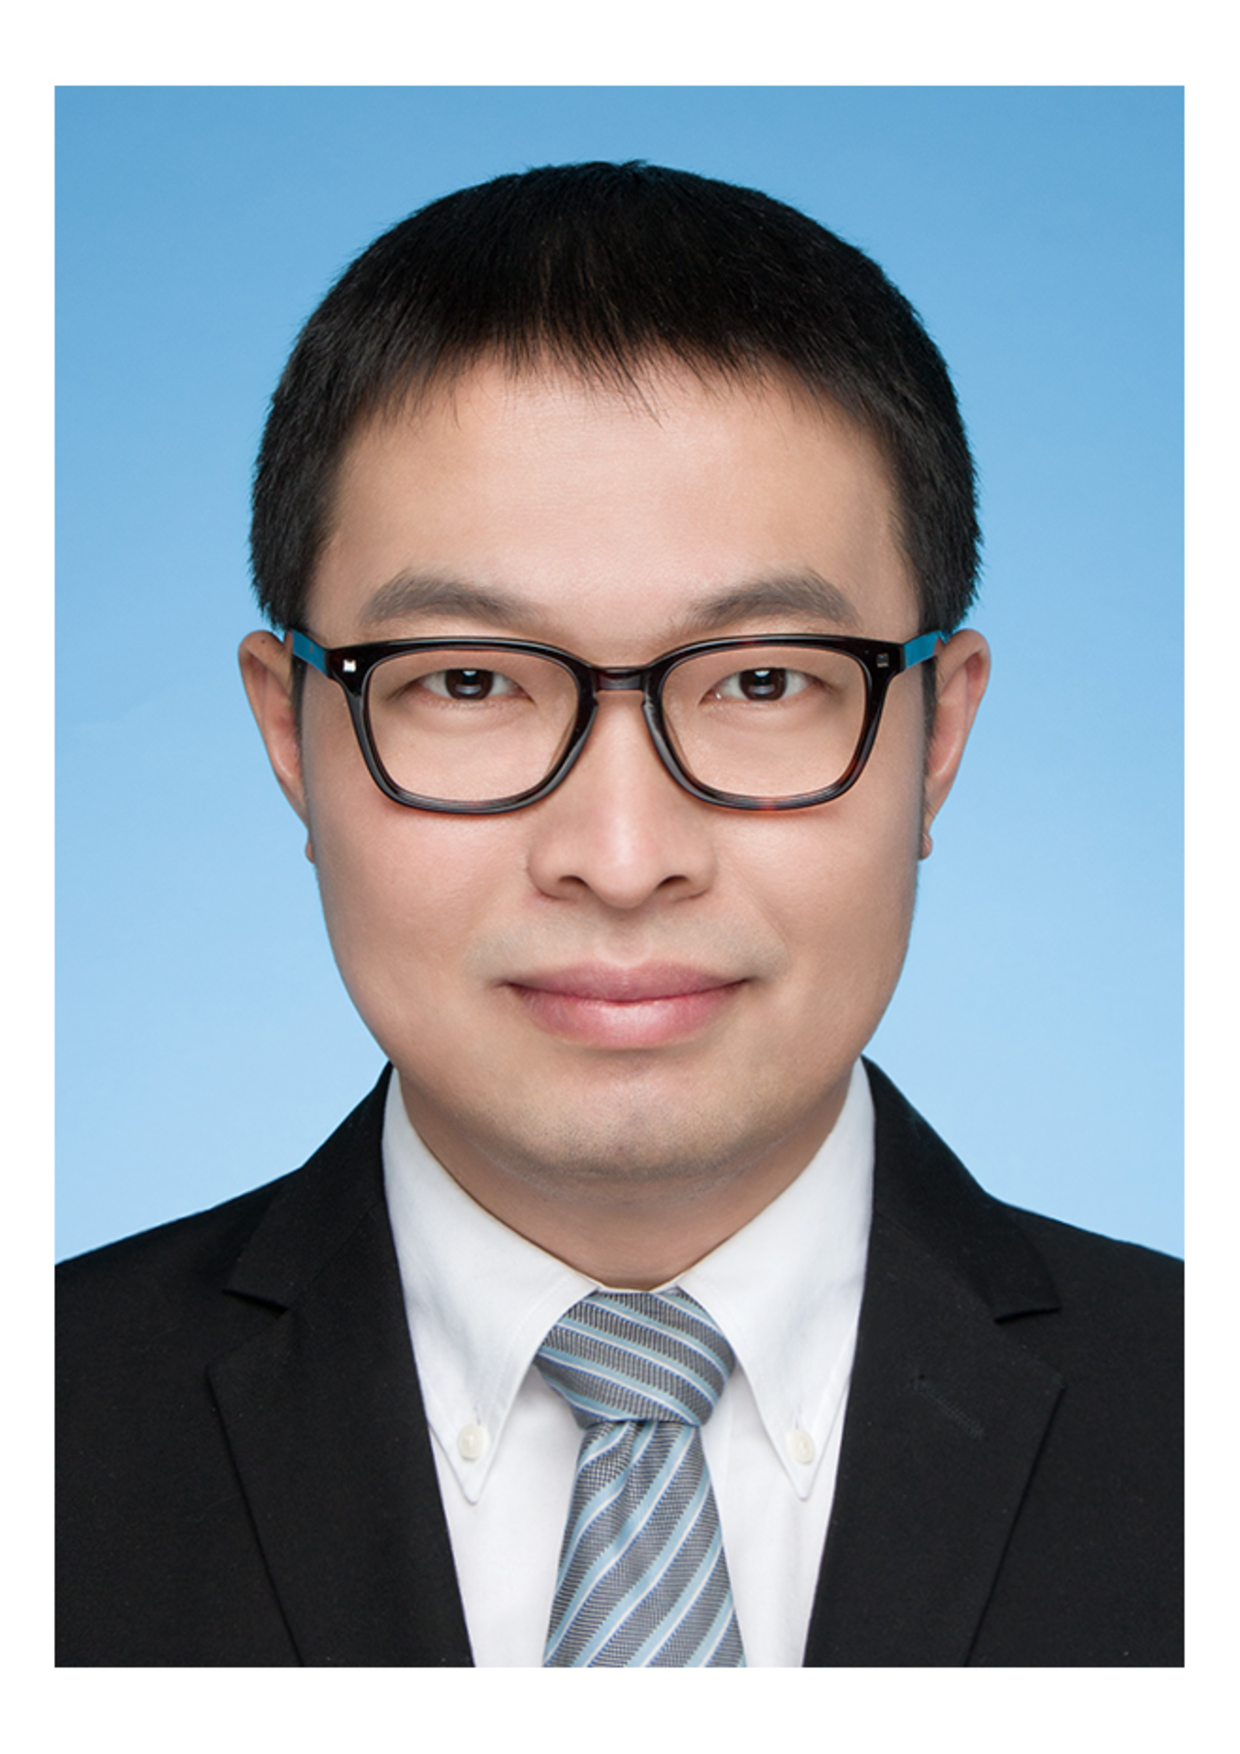
\includegraphics[width=1in,height=1.25in,clip,keepaspectratio]{./fig/author/Tao_Song}}]{Tao Song}
is currently working as a postdoc at Shanghai Jiao Tong University in China. He received his Ph.D. degree in computer science and M.Eng. degree in software engineering from Shanghai Jiao Tong University. His research interests include data center networking, cloud computing, artificial intelligence and swarm intelligence.
\end{IEEEbiography}

\begin{IEEEbiography}[{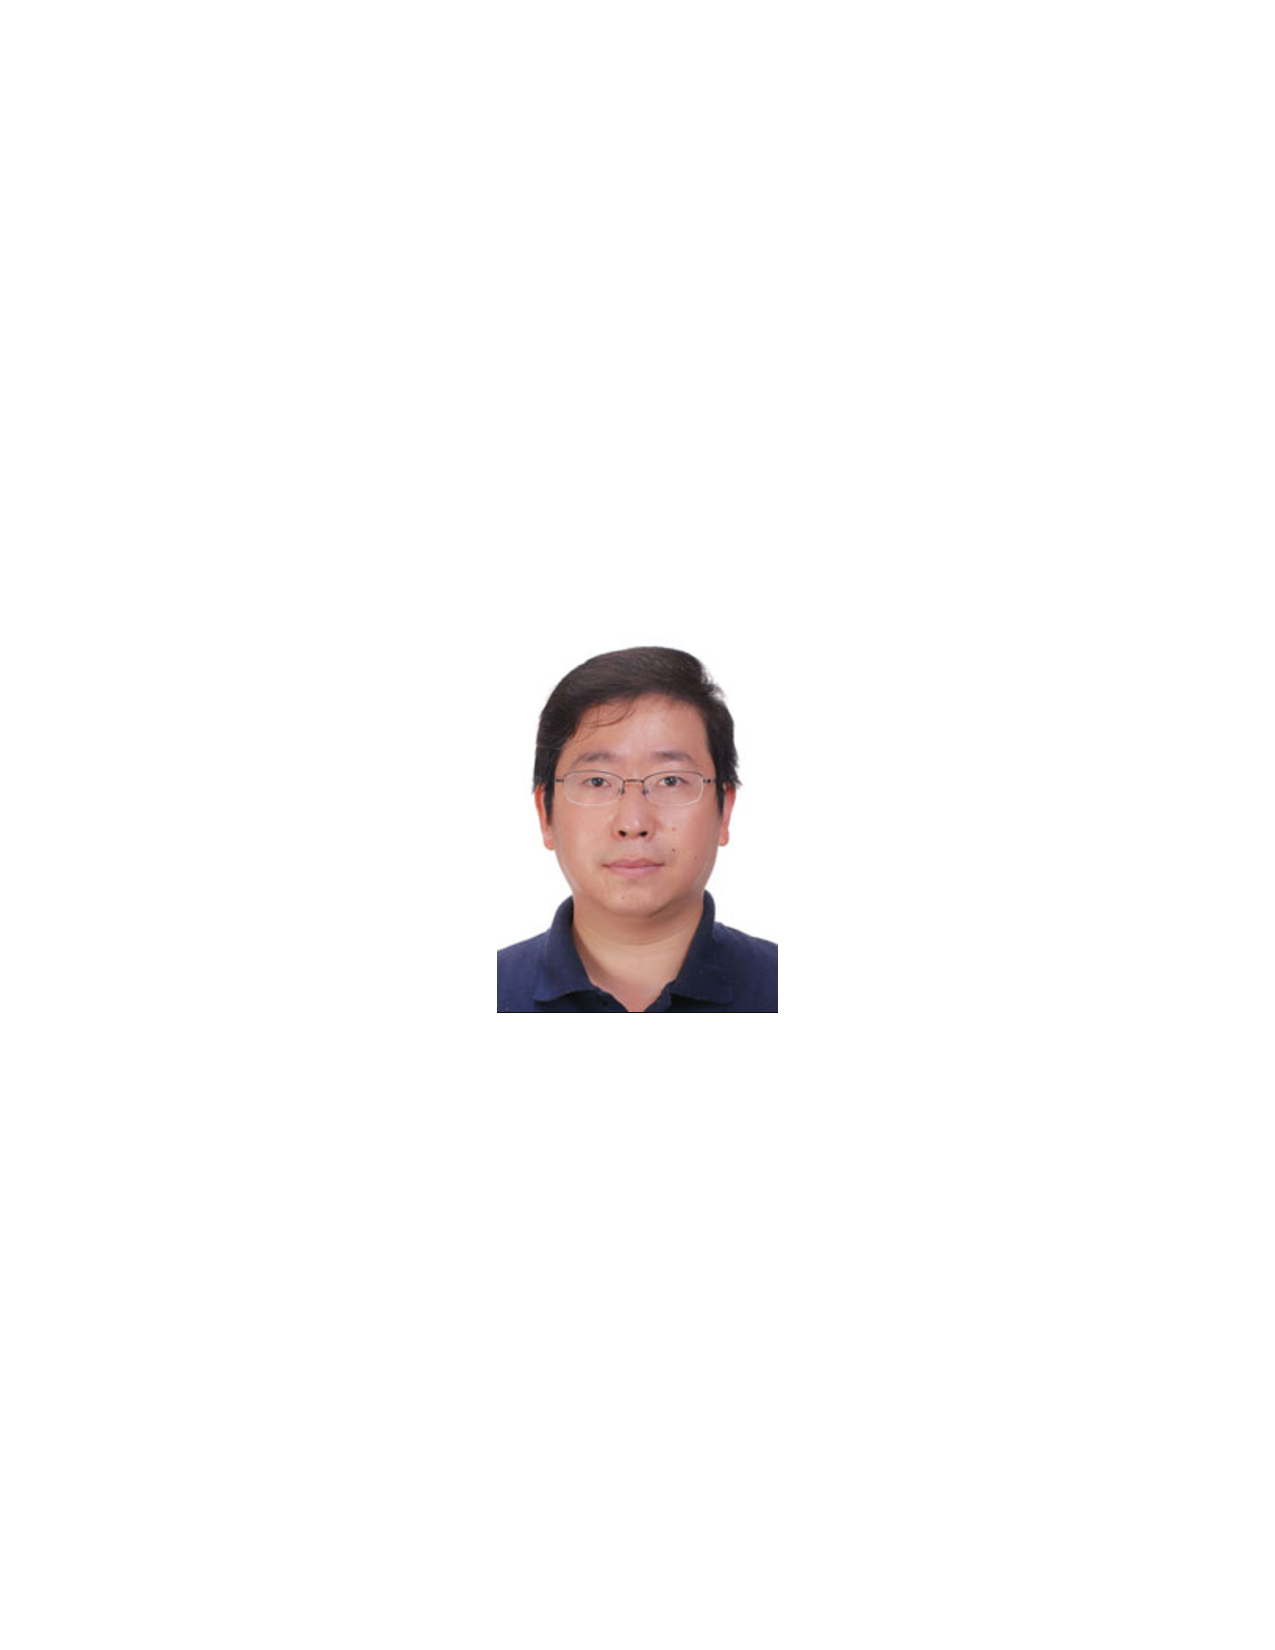
\includegraphics[width=1in,height=1.25in,clip,keepaspectratio]{./fig/author/Zhengwei_Qi}}]{Zhengwei Qi}
received the BEng and MEng degrees from Northwestern Polytechnical University, in 1999 and 2002, and the PhD degree from Shanghai Jiao Tong University, in 2005. Currently, he is a professor in the School of Software, Shanghai Jiao Tong University (China). His research interests include distributed computing, virtualized security, model checking, program analysis and embedded systems.
\end{IEEEbiography}

\begin{IEEEbiography}[{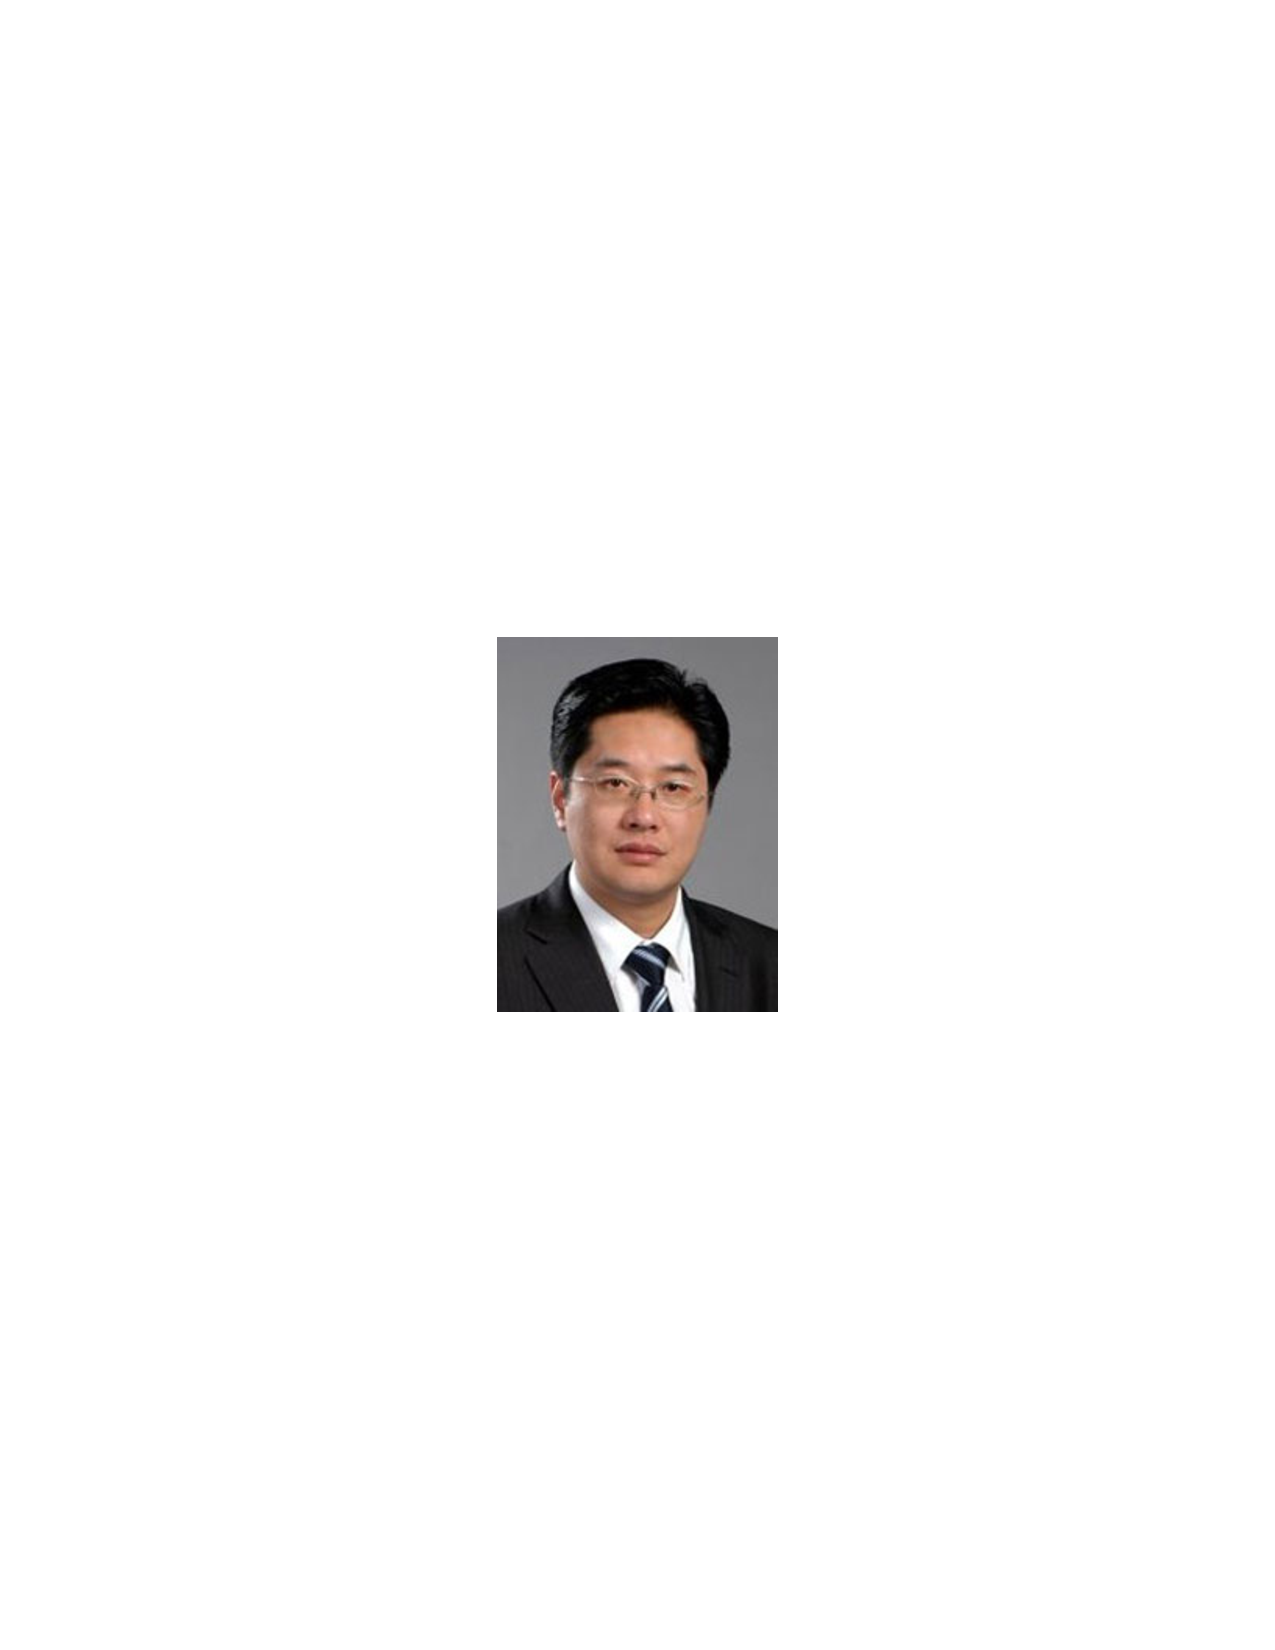
\includegraphics[width=1in,height=1.25in,clip,keepaspectratio]{./fig/author/Haibing_Guan}}]{Haibing Guan}
received the PhD degree from Tongji University, in 1999. He is a professor of School of Electronic, Information and Electronic Engineering, Shanghai Jiao Tong University, and the director of the Shanghai Key Laboratory of Scalable Computing and Systems. His research interests include distributed computing, network security, network storage, green IT, and cloud computing.
\end{IEEEbiography}

% % if you will not have a photo at all:
% \begin{IEEEbiographynophoto}{John Doe}
% Biography text here.
% \end{IEEEbiographynophoto}

% % insert where needed to balance the two columns on the last page with
% % biographies
% %\newpage

% \begin{IEEEbiographynophoto}{Jane Doe}
% Biography text here.
% \end{IEEEbiographynophoto}

% You can push biographies down or up by placing
% a \vfill before or after them. The appropriate
% use of \vfill depends on what kind of text is
% on the last page and whether or not the columns
% are being equalized.

%\vfill

% Can be used to pull up biographies so that the bottom of the last one
% is flush with the other column.
%\enlargethispage{-5in}



% that's all folks
\end{document}


